\documentclass[twoside]{book}

% Packages required by doxygen
\usepackage{fixltx2e}
\usepackage{calc}
\usepackage{doxygen}
\usepackage{graphicx}
\usepackage[utf8]{inputenc}
\usepackage{makeidx}
\usepackage{multicol}
\usepackage{multirow}
\PassOptionsToPackage{warn}{textcomp}
\usepackage{textcomp}
\usepackage[nointegrals]{wasysym}
\usepackage[table]{xcolor}

% Font selection
\usepackage[T1]{fontenc}
\usepackage{mathptmx}
\usepackage[scaled=.90]{helvet}
\usepackage{courier}
\usepackage{amssymb}
\usepackage{sectsty}
\renewcommand{\familydefault}{\sfdefault}
\allsectionsfont{%
  \fontseries{bc}\selectfont%
  \color{darkgray}%
}
\renewcommand{\DoxyLabelFont}{%
  \fontseries{bc}\selectfont%
  \color{darkgray}%
}
\newcommand{\+}{\discretionary{\mbox{\scriptsize$\hookleftarrow$}}{}{}}

% Page & text layout
\usepackage{geometry}
\geometry{%
  a4paper,%
  top=2.5cm,%
  bottom=2.5cm,%
  left=2.5cm,%
  right=2.5cm%
}
\tolerance=750
\hfuzz=15pt
\hbadness=750
\setlength{\emergencystretch}{15pt}
\setlength{\parindent}{0cm}
\setlength{\parskip}{0.2cm}
\makeatletter
\renewcommand{\paragraph}{%
  \@startsection{paragraph}{4}{0ex}{-1.0ex}{1.0ex}{%
    \normalfont\normalsize\bfseries\SS@parafont%
  }%
}
\renewcommand{\subparagraph}{%
  \@startsection{subparagraph}{5}{0ex}{-1.0ex}{1.0ex}{%
    \normalfont\normalsize\bfseries\SS@subparafont%
  }%
}
\makeatother

% Headers & footers
\usepackage{fancyhdr}
\pagestyle{fancyplain}
\fancyhead[LE]{\fancyplain{}{\bfseries\thepage}}
\fancyhead[CE]{\fancyplain{}{}}
\fancyhead[RE]{\fancyplain{}{\bfseries\leftmark}}
\fancyhead[LO]{\fancyplain{}{\bfseries\rightmark}}
\fancyhead[CO]{\fancyplain{}{}}
\fancyhead[RO]{\fancyplain{}{\bfseries\thepage}}
\fancyfoot[LE]{\fancyplain{}{}}
\fancyfoot[CE]{\fancyplain{}{}}
\fancyfoot[RE]{\fancyplain{}{\bfseries\scriptsize Generated on Fri Oct 3 2014 17\+:46\+:16 for N3 -\/ C\+G by Doxygen }}
\fancyfoot[LO]{\fancyplain{}{\bfseries\scriptsize Generated on Fri Oct 3 2014 17\+:46\+:16 for N3 -\/ C\+G by Doxygen }}
\fancyfoot[CO]{\fancyplain{}{}}
\fancyfoot[RO]{\fancyplain{}{}}
\renewcommand{\footrulewidth}{0.4pt}
\renewcommand{\chaptermark}[1]{%
  \markboth{#1}{}%
}
\renewcommand{\sectionmark}[1]{%
  \markright{\thesection\ #1}%
}

% Indices & bibliography
\usepackage{natbib}
\usepackage[titles]{tocloft}
\setcounter{tocdepth}{3}
\setcounter{secnumdepth}{5}
\makeindex

% Hyperlinks (required, but should be loaded last)
\usepackage{ifpdf}
\ifpdf
  \usepackage[pdftex,pagebackref=true]{hyperref}
\else
  \usepackage[ps2pdf,pagebackref=true]{hyperref}
\fi
\hypersetup{%
  colorlinks=true,%
  linkcolor=blue,%
  citecolor=blue,%
  unicode%
}

% Custom commands
\newcommand{\clearemptydoublepage}{%
  \newpage{\pagestyle{empty}\cleardoublepage}%
}


%===== C O N T E N T S =====

\begin{document}

% Titlepage & ToC
\hypersetup{pageanchor=false,
             bookmarks=true,
             bookmarksnumbered=true,
             pdfencoding=unicode
            }
\pagenumbering{roman}
\begin{titlepage}
\vspace*{7cm}
\begin{center}%
{\Large N3 -\/ C\+G }\\
\vspace*{1cm}
{\large Generated by Doxygen 1.8.8}\\
\vspace*{0.5cm}
{\small Fri Oct 3 2014 17:46:16}\\
\end{center}
\end{titlepage}
\clearemptydoublepage
\tableofcontents
\clearemptydoublepage
\pagenumbering{arabic}
\hypersetup{pageanchor=true}

%--- Begin generated contents ---
\chapter{Hierarchical Index}
\section{Class Hierarchy}
This inheritance list is sorted roughly, but not completely, alphabetically\+:\begin{DoxyCompactList}
\item \contentsline{section}{Abstract\+Callback}{\pageref{classAbstractCallback}}{}
\begin{DoxyCompactList}
\item \contentsline{section}{Adicao\+Callback}{\pageref{classAdicaoCallback}}{}
\item \contentsline{section}{Edicao\+Callback}{\pageref{classEdicaoCallback}}{}
\end{DoxyCompactList}
\item \contentsline{section}{B\+Box}{\pageref{classBBox}}{}
\item \contentsline{section}{Camera}{\pageref{classCamera}}{}
\item \contentsline{section}{Cor}{\pageref{classCor}}{}
\item \contentsline{section}{Mundo}{\pageref{classMundo}}{}
\item \contentsline{section}{Objeto\+Grafico}{\pageref{classObjetoGrafico}}{}
\item \contentsline{section}{Ponto}{\pageref{classPonto}}{}
\item \contentsline{section}{Transformacao}{\pageref{classTransformacao}}{}
\end{DoxyCompactList}

\chapter{Class Index}
\section{Class List}
Here are the classes, structs, unions and interfaces with brief descriptions\+:\begin{DoxyCompactList}
\item\contentsline{section}{\hyperlink{classAbstractCallback}{Abstract\+Callback} \\*Classe abstrata para lidar com os eventos dependendo do estado }{\pageref{classAbstractCallback}}{}
\item\contentsline{section}{\hyperlink{classAdicaoCallback}{Adicao\+Callback} \\*Estado da aplicação com relação aos momentos de adição }{\pageref{classAdicaoCallback}}{}
\item\contentsline{section}{\hyperlink{classBBox}{B\+Box} \\*Uma Bounding\+Box usada para delimitar um objeto gáfico }{\pageref{classBBox}}{}
\item\contentsline{section}{\hyperlink{classCamera}{Camera} \\*A camera da cena grafica }{\pageref{classCamera}}{}
\item\contentsline{section}{\hyperlink{classCor}{Cor} \\*Uma cor R\+G\+B }{\pageref{classCor}}{}
\item\contentsline{section}{\hyperlink{classEdicaoCallback}{Edicao\+Callback} \\*Estado da aplicação com relação aos momentos de edição }{\pageref{classEdicaoCallback}}{}
\item\contentsline{section}{\hyperlink{classMundo}{Mundo} \\*O Universo gráfico }{\pageref{classMundo}}{}
\item\contentsline{section}{\hyperlink{classObjetoGrafico}{Objeto\+Grafico} \\*Um Objeto Grafico do mundo }{\pageref{classObjetoGrafico}}{}
\item\contentsline{section}{\hyperlink{classPonto}{Ponto} \\*\hyperlink{classPonto}{Ponto} 3\+D }{\pageref{classPonto}}{}
\item\contentsline{section}{\hyperlink{classTransformacao}{Transformacao} \\*Uma transformação linear }{\pageref{classTransformacao}}{}
\end{DoxyCompactList}

\chapter{File Index}
\section{File List}
Here is a list of all files with brief descriptions\+:\begin{DoxyCompactList}
\item\contentsline{section}{\hyperlink{AbstractCallback_8cpp}{Abstract\+Callback.\+cpp} }{\pageref{AbstractCallback_8cpp}}{}
\item\contentsline{section}{\hyperlink{AbstractCallback_8hpp}{Abstract\+Callback.\+hpp} \\*Definição abstrata da classe da aplicação }{\pageref{AbstractCallback_8hpp}}{}
\item\contentsline{section}{\hyperlink{AdicaoCallback_8cpp}{Adicao\+Callback.\+cpp} }{\pageref{AdicaoCallback_8cpp}}{}
\item\contentsline{section}{\hyperlink{AdicaoCallback_8hpp}{Adicao\+Callback.\+hpp} \\*Definição do estado de adição }{\pageref{AdicaoCallback_8hpp}}{}
\item\contentsline{section}{\hyperlink{BBox_8cpp}{B\+Box.\+cpp} }{\pageref{BBox_8cpp}}{}
\item\contentsline{section}{\hyperlink{BBox_8hpp}{B\+Box.\+hpp} \\*Definição da \hyperlink{classBBox}{B\+Box} }{\pageref{BBox_8hpp}}{}
\item\contentsline{section}{\hyperlink{Camera_8cpp}{Camera.\+cpp} }{\pageref{Camera_8cpp}}{}
\item\contentsline{section}{\hyperlink{Camera_8hpp}{Camera.\+hpp} }{\pageref{Camera_8hpp}}{}
\item\contentsline{section}{\hyperlink{Cor_8cpp}{Cor.\+cpp} }{\pageref{Cor_8cpp}}{}
\item\contentsline{section}{\hyperlink{Cor_8hpp}{Cor.\+hpp} \\*Definição de \hyperlink{classCamera}{Camera} }{\pageref{Cor_8hpp}}{}
\item\contentsline{section}{\hyperlink{EdicaoCallback_8cpp}{Edicao\+Callback.\+cpp} }{\pageref{EdicaoCallback_8cpp}}{}
\item\contentsline{section}{\hyperlink{EdicaoCallback_8hpp}{Edicao\+Callback.\+hpp} \\*Definição do estado de edição }{\pageref{EdicaoCallback_8hpp}}{}
\item\contentsline{section}{\hyperlink{Main_8cpp}{Main.\+cpp} }{\pageref{Main_8cpp}}{}
\item\contentsline{section}{\hyperlink{Mundo_8cpp}{Mundo.\+cpp} }{\pageref{Mundo_8cpp}}{}
\item\contentsline{section}{\hyperlink{Mundo_8hpp}{Mundo.\+hpp} \\*Definição de \hyperlink{classMundo}{Mundo} par o Trabalho N3 de C\+G }{\pageref{Mundo_8hpp}}{}
\item\contentsline{section}{\hyperlink{ObjetoGrafico_8cpp}{Objeto\+Grafico.\+cpp} }{\pageref{ObjetoGrafico_8cpp}}{}
\item\contentsline{section}{\hyperlink{ObjetoGrafico_8hpp}{Objeto\+Grafico.\+hpp} \\*Definição de Ojeto Gráfico }{\pageref{ObjetoGrafico_8hpp}}{}
\item\contentsline{section}{\hyperlink{Ponto_8cpp}{Ponto.\+cpp} }{\pageref{Ponto_8cpp}}{}
\item\contentsline{section}{\hyperlink{Ponto_8hpp}{Ponto.\+hpp} \\*Definicao de \hyperlink{classPonto}{Ponto} }{\pageref{Ponto_8hpp}}{}
\item\contentsline{section}{\hyperlink{Transformacao_8cpp}{Transformacao.\+cpp} }{\pageref{Transformacao_8cpp}}{}
\item\contentsline{section}{\hyperlink{Transformacao_8hpp}{Transformacao.\+hpp} \\*Definição de \hyperlink{classTransformacao}{Transformacao} }{\pageref{Transformacao_8hpp}}{}
\item\contentsline{section}{\hyperlink{Utils_8cpp}{Utils.\+cpp} }{\pageref{Utils_8cpp}}{}
\item\contentsline{section}{\hyperlink{Utils_8hpp}{Utils.\+hpp} }{\pageref{Utils_8hpp}}{}
\end{DoxyCompactList}

\chapter{Class Documentation}
\hypertarget{classAbstractCallback}{\section{Abstract\+Callback Class Reference}
\label{classAbstractCallback}\index{Abstract\+Callback@{Abstract\+Callback}}
}


Classe abstrata para lidar com os eventos dependendo do estado.  




{\ttfamily \#include $<$Abstract\+Callback.\+hpp$>$}



Inheritance diagram for Abstract\+Callback\+:
\nopagebreak
\begin{figure}[H]
\begin{center}
\leavevmode
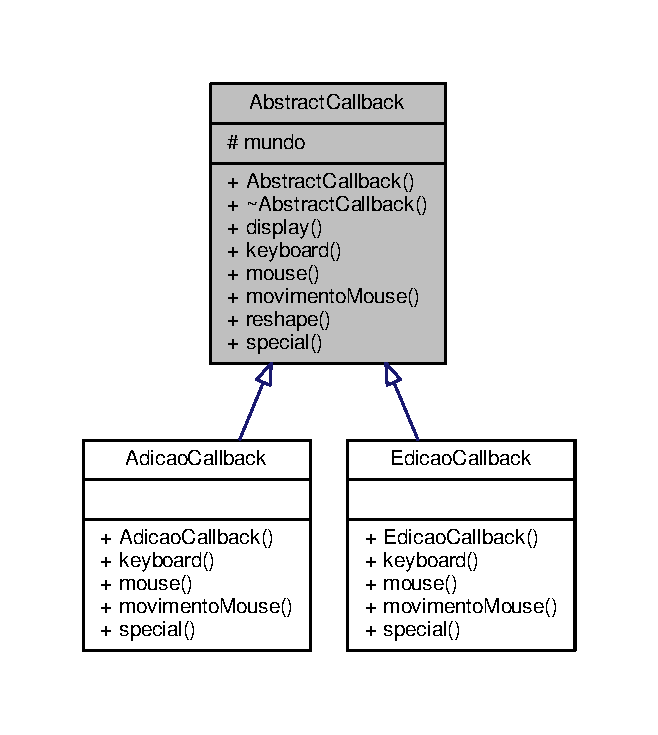
\includegraphics[width=316pt]{classAbstractCallback__inherit__graph}
\end{center}
\end{figure}


Collaboration diagram for Abstract\+Callback\+:
\nopagebreak
\begin{figure}[H]
\begin{center}
\leavevmode
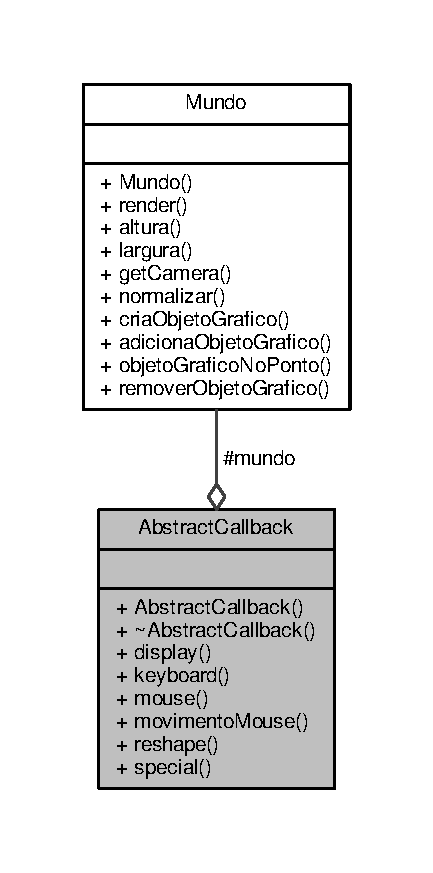
\includegraphics[width=208pt]{classAbstractCallback__coll__graph}
\end{center}
\end{figure}
\subsection*{Public Member Functions}
\begin{DoxyCompactItemize}
\item 
\hyperlink{classAbstractCallback_ab410b1edcdfab5a74298edb8ee9cb4a9}{Abstract\+Callback} (\hyperlink{classMundo}{Mundo} \&\hyperlink{classAbstractCallback_a17c2460462c7e985368ef227338d3430}{mundo})
\item 
virtual \hyperlink{classAbstractCallback_a5ae7f5e51738a94b7dab97555babf40d}{$\sim$\+Abstract\+Callback} ()
\item 
virtual void \hyperlink{classAbstractCallback_aabd79b70b927b64276000d3d17959841}{display} ()
\item 
virtual void \hyperlink{classAbstractCallback_af897d4ee16944785ddb2d90ffad155b2}{keyboard} (unsigned char key, const \hyperlink{classPonto}{Ponto} \&point)
\item 
virtual void \hyperlink{classAbstractCallback_a1c30a14b8f6212712152364a6620760d}{mouse} (int button, int state, const \hyperlink{classPonto}{Ponto} \&point)=0
\item 
virtual void \hyperlink{classAbstractCallback_a6a13a67f479eb87c0416d1464b8ef37a}{movimento\+Mouse} (const \hyperlink{classPonto}{Ponto} \&ponto)=0
\item 
virtual void \hyperlink{classAbstractCallback_a649127b2eccaccc9e201073944f65e8c}{reshape} (int width, int height)
\item 
virtual void \hyperlink{classAbstractCallback_a92270c46a72e1b36f8ad72a26f7c37dd}{special} (int key, const \hyperlink{classPonto}{Ponto} \&point)=0
\end{DoxyCompactItemize}
\subsection*{Protected Attributes}
\begin{DoxyCompactItemize}
\item 
\hyperlink{classMundo}{Mundo} \& \hyperlink{classAbstractCallback_a17c2460462c7e985368ef227338d3430}{mundo}
\end{DoxyCompactItemize}


\subsection{Detailed Description}
Classe abstrata para lidar com os eventos dependendo do estado. 

\begin{DoxyAuthor}{Author}
Arthur Henrique Eggert 
\end{DoxyAuthor}
\begin{DoxyDate}{Date}
2014-\/09-\/21 
\end{DoxyDate}


\subsection{Constructor \& Destructor Documentation}
\hypertarget{classAbstractCallback_ab410b1edcdfab5a74298edb8ee9cb4a9}{\index{Abstract\+Callback@{Abstract\+Callback}!Abstract\+Callback@{Abstract\+Callback}}
\index{Abstract\+Callback@{Abstract\+Callback}!Abstract\+Callback@{Abstract\+Callback}}
\subsubsection[{Abstract\+Callback}]{\setlength{\rightskip}{0pt plus 5cm}Abstract\+Callback\+::\+Abstract\+Callback (
\begin{DoxyParamCaption}
\item[{{\bf Mundo} \&}]{mundo}
\end{DoxyParamCaption}
)}}\label{classAbstractCallback_ab410b1edcdfab5a74298edb8ee9cb4a9}
Cria um estado para a manipulação do mundo grafico \hypertarget{classAbstractCallback_a5ae7f5e51738a94b7dab97555babf40d}{\index{Abstract\+Callback@{Abstract\+Callback}!````~Abstract\+Callback@{$\sim$\+Abstract\+Callback}}
\index{````~Abstract\+Callback@{$\sim$\+Abstract\+Callback}!Abstract\+Callback@{Abstract\+Callback}}
\subsubsection[{$\sim$\+Abstract\+Callback}]{\setlength{\rightskip}{0pt plus 5cm}Abstract\+Callback\+::$\sim$\+Abstract\+Callback (
\begin{DoxyParamCaption}
{}
\end{DoxyParamCaption}
)\hspace{0.3cm}{\ttfamily [virtual]}}}\label{classAbstractCallback_a5ae7f5e51738a94b7dab97555babf40d}
Destroi este estado da aplicacao. 

\subsection{Member Function Documentation}
\hypertarget{classAbstractCallback_aabd79b70b927b64276000d3d17959841}{\index{Abstract\+Callback@{Abstract\+Callback}!display@{display}}
\index{display@{display}!Abstract\+Callback@{Abstract\+Callback}}
\subsubsection[{display}]{\setlength{\rightskip}{0pt plus 5cm}void Abstract\+Callback\+::display (
\begin{DoxyParamCaption}
{}
\end{DoxyParamCaption}
)\hspace{0.3cm}{\ttfamily [virtual]}}}\label{classAbstractCallback_aabd79b70b927b64276000d3d17959841}
Faz o display do \hyperlink{classMundo}{Mundo} Grafico. \hypertarget{classAbstractCallback_af897d4ee16944785ddb2d90ffad155b2}{\index{Abstract\+Callback@{Abstract\+Callback}!keyboard@{keyboard}}
\index{keyboard@{keyboard}!Abstract\+Callback@{Abstract\+Callback}}
\subsubsection[{keyboard}]{\setlength{\rightskip}{0pt plus 5cm}void Abstract\+Callback\+::keyboard (
\begin{DoxyParamCaption}
\item[{unsigned char}]{key, }
\item[{const {\bf Ponto} \&}]{point}
\end{DoxyParamCaption}
)\hspace{0.3cm}{\ttfamily [virtual]}}}\label{classAbstractCallback_af897d4ee16944785ddb2d90ffad155b2}
Callback de Teclado 

Reimplemented in \hyperlink{classEdicaoCallback_ab2d6a4a0e971628e460e7505ff289ac9}{Edicao\+Callback}, and \hyperlink{classAdicaoCallback_a1161a0292e30660bbc653dd830ed7e78}{Adicao\+Callback}.

\hypertarget{classAbstractCallback_a1c30a14b8f6212712152364a6620760d}{\index{Abstract\+Callback@{Abstract\+Callback}!mouse@{mouse}}
\index{mouse@{mouse}!Abstract\+Callback@{Abstract\+Callback}}
\subsubsection[{mouse}]{\setlength{\rightskip}{0pt plus 5cm}virtual void Abstract\+Callback\+::mouse (
\begin{DoxyParamCaption}
\item[{int}]{button, }
\item[{int}]{state, }
\item[{const {\bf Ponto} \&}]{point}
\end{DoxyParamCaption}
)\hspace{0.3cm}{\ttfamily [pure virtual]}}}\label{classAbstractCallback_a1c30a14b8f6212712152364a6620760d}
Callback de Mouse 

Implemented in \hyperlink{classEdicaoCallback_ad3a885decb234555569dbb3d26f0dcdd}{Edicao\+Callback}, and \hyperlink{classAdicaoCallback_ac1a328393245c840b20bd78535786aad}{Adicao\+Callback}.

\hypertarget{classAbstractCallback_a6a13a67f479eb87c0416d1464b8ef37a}{\index{Abstract\+Callback@{Abstract\+Callback}!movimento\+Mouse@{movimento\+Mouse}}
\index{movimento\+Mouse@{movimento\+Mouse}!Abstract\+Callback@{Abstract\+Callback}}
\subsubsection[{movimento\+Mouse}]{\setlength{\rightskip}{0pt plus 5cm}virtual void Abstract\+Callback\+::movimento\+Mouse (
\begin{DoxyParamCaption}
\item[{const {\bf Ponto} \&}]{ponto}
\end{DoxyParamCaption}
)\hspace{0.3cm}{\ttfamily [pure virtual]}}}\label{classAbstractCallback_a6a13a67f479eb87c0416d1464b8ef37a}
Callback do movimento de mouse 

Implemented in \hyperlink{classEdicaoCallback_a58507cc2d8f1e0774fc15aa1d2adca92}{Edicao\+Callback}, and \hyperlink{classAdicaoCallback_a4fe49be2210d8b9ef60421e9e0c517bf}{Adicao\+Callback}.

\hypertarget{classAbstractCallback_a649127b2eccaccc9e201073944f65e8c}{\index{Abstract\+Callback@{Abstract\+Callback}!reshape@{reshape}}
\index{reshape@{reshape}!Abstract\+Callback@{Abstract\+Callback}}
\subsubsection[{reshape}]{\setlength{\rightskip}{0pt plus 5cm}void Abstract\+Callback\+::reshape (
\begin{DoxyParamCaption}
\item[{int}]{width, }
\item[{int}]{height}
\end{DoxyParamCaption}
)\hspace{0.3cm}{\ttfamily [virtual]}}}\label{classAbstractCallback_a649127b2eccaccc9e201073944f65e8c}
Callback do redimencionamento da tela \hypertarget{classAbstractCallback_a92270c46a72e1b36f8ad72a26f7c37dd}{\index{Abstract\+Callback@{Abstract\+Callback}!special@{special}}
\index{special@{special}!Abstract\+Callback@{Abstract\+Callback}}
\subsubsection[{special}]{\setlength{\rightskip}{0pt plus 5cm}virtual void Abstract\+Callback\+::special (
\begin{DoxyParamCaption}
\item[{int}]{key, }
\item[{const {\bf Ponto} \&}]{point}
\end{DoxyParamCaption}
)\hspace{0.3cm}{\ttfamily [pure virtual]}}}\label{classAbstractCallback_a92270c46a72e1b36f8ad72a26f7c37dd}
Calbback para teclas especias do teclado 

Implemented in \hyperlink{classEdicaoCallback_ab3af9b7362efe5d4a8ec18cf840f66c0}{Edicao\+Callback}, and \hyperlink{classAdicaoCallback_adf5c6d3c487342ea989b7716db834684}{Adicao\+Callback}.



\subsection{Member Data Documentation}
\hypertarget{classAbstractCallback_a17c2460462c7e985368ef227338d3430}{\index{Abstract\+Callback@{Abstract\+Callback}!mundo@{mundo}}
\index{mundo@{mundo}!Abstract\+Callback@{Abstract\+Callback}}
\subsubsection[{mundo}]{\setlength{\rightskip}{0pt plus 5cm}{\bf Mundo}\& Abstract\+Callback\+::mundo\hspace{0.3cm}{\ttfamily [protected]}}}\label{classAbstractCallback_a17c2460462c7e985368ef227338d3430}


The documentation for this class was generated from the following files\+:\begin{DoxyCompactItemize}
\item 
\hyperlink{AbstractCallback_8hpp}{Abstract\+Callback.\+hpp}\item 
\hyperlink{AbstractCallback_8cpp}{Abstract\+Callback.\+cpp}\end{DoxyCompactItemize}

\hypertarget{classAdicaoCallback}{\section{Adicao\+Callback Class Reference}
\label{classAdicaoCallback}\index{Adicao\+Callback@{Adicao\+Callback}}
}


Estado da aplicação com relação aos momentos de adição.  




{\ttfamily \#include $<$Adicao\+Callback.\+hpp$>$}



Inheritance diagram for Adicao\+Callback\+:
\nopagebreak
\begin{figure}[H]
\begin{center}
\leavevmode
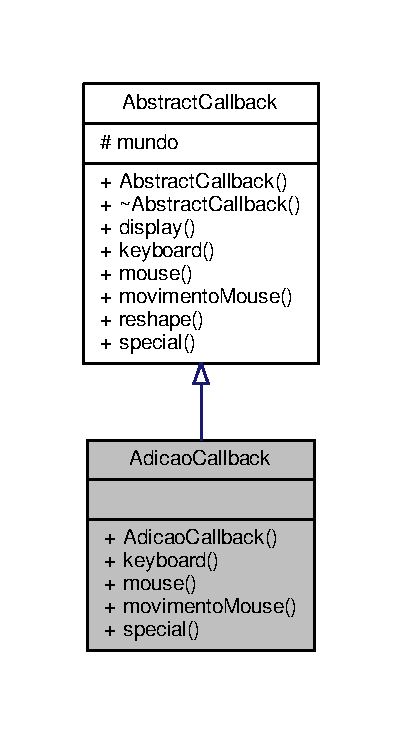
\includegraphics[width=193pt]{classAdicaoCallback__inherit__graph}
\end{center}
\end{figure}


Collaboration diagram for Adicao\+Callback\+:
\nopagebreak
\begin{figure}[H]
\begin{center}
\leavevmode
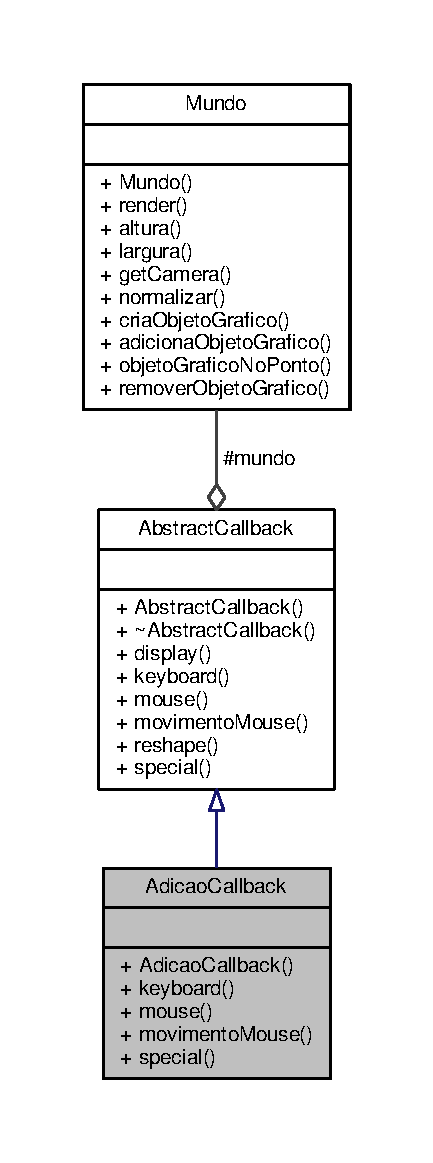
\includegraphics[height=550pt]{classAdicaoCallback__coll__graph}
\end{center}
\end{figure}
\subsection*{Public Member Functions}
\begin{DoxyCompactItemize}
\item 
\hyperlink{classAdicaoCallback_a7576b50f747918fcfe1ecbb41ecd0326}{Adicao\+Callback} (\hyperlink{classMundo}{Mundo} \&\hyperlink{classAbstractCallback_a17c2460462c7e985368ef227338d3430}{mundo})
\item 
virtual void \hyperlink{classAdicaoCallback_a1161a0292e30660bbc653dd830ed7e78}{keyboard} (unsigned char key, const \hyperlink{classPonto}{Ponto} \&point)
\item 
virtual void \hyperlink{classAdicaoCallback_ac1a328393245c840b20bd78535786aad}{mouse} (int button, int state, const \hyperlink{classPonto}{Ponto} \&point)
\item 
virtual void \hyperlink{classAdicaoCallback_a4fe49be2210d8b9ef60421e9e0c517bf}{movimento\+Mouse} (const \hyperlink{classPonto}{Ponto} \&point)
\item 
virtual void \hyperlink{classAdicaoCallback_adf5c6d3c487342ea989b7716db834684}{special} (int key, const \hyperlink{classPonto}{Ponto} \&point)
\end{DoxyCompactItemize}
\subsection*{Additional Inherited Members}


\subsection{Detailed Description}
Estado da aplicação com relação aos momentos de adição. 

\begin{DoxyAuthor}{Author}
Arthur Henrique Eggert 
\end{DoxyAuthor}
\begin{DoxyDate}{Date}
2014-\/09-\/21 
\end{DoxyDate}


\subsection{Constructor \& Destructor Documentation}
\hypertarget{classAdicaoCallback_a7576b50f747918fcfe1ecbb41ecd0326}{\index{Adicao\+Callback@{Adicao\+Callback}!Adicao\+Callback@{Adicao\+Callback}}
\index{Adicao\+Callback@{Adicao\+Callback}!Adicao\+Callback@{Adicao\+Callback}}
\subsubsection[{Adicao\+Callback}]{\setlength{\rightskip}{0pt plus 5cm}Adicao\+Callback\+::\+Adicao\+Callback (
\begin{DoxyParamCaption}
\item[{{\bf Mundo} \&}]{mundo}
\end{DoxyParamCaption}
)}}\label{classAdicaoCallback_a7576b50f747918fcfe1ecbb41ecd0326}


\subsection{Member Function Documentation}
\hypertarget{classAdicaoCallback_a1161a0292e30660bbc653dd830ed7e78}{\index{Adicao\+Callback@{Adicao\+Callback}!keyboard@{keyboard}}
\index{keyboard@{keyboard}!Adicao\+Callback@{Adicao\+Callback}}
\subsubsection[{keyboard}]{\setlength{\rightskip}{0pt plus 5cm}void Adicao\+Callback\+::keyboard (
\begin{DoxyParamCaption}
\item[{unsigned char}]{key, }
\item[{const {\bf Ponto} \&}]{point}
\end{DoxyParamCaption}
)\hspace{0.3cm}{\ttfamily [virtual]}}}\label{classAdicaoCallback_a1161a0292e30660bbc653dd830ed7e78}
Callback de Teclado 

Reimplemented from \hyperlink{classAbstractCallback_af897d4ee16944785ddb2d90ffad155b2}{Abstract\+Callback}.

\hypertarget{classAdicaoCallback_ac1a328393245c840b20bd78535786aad}{\index{Adicao\+Callback@{Adicao\+Callback}!mouse@{mouse}}
\index{mouse@{mouse}!Adicao\+Callback@{Adicao\+Callback}}
\subsubsection[{mouse}]{\setlength{\rightskip}{0pt plus 5cm}void Adicao\+Callback\+::mouse (
\begin{DoxyParamCaption}
\item[{int}]{button, }
\item[{int}]{state, }
\item[{const {\bf Ponto} \&}]{point}
\end{DoxyParamCaption}
)\hspace{0.3cm}{\ttfamily [virtual]}}}\label{classAdicaoCallback_ac1a328393245c840b20bd78535786aad}
Callback de Mouse 

Implements \hyperlink{classAbstractCallback_a1c30a14b8f6212712152364a6620760d}{Abstract\+Callback}.

\hypertarget{classAdicaoCallback_a4fe49be2210d8b9ef60421e9e0c517bf}{\index{Adicao\+Callback@{Adicao\+Callback}!movimento\+Mouse@{movimento\+Mouse}}
\index{movimento\+Mouse@{movimento\+Mouse}!Adicao\+Callback@{Adicao\+Callback}}
\subsubsection[{movimento\+Mouse}]{\setlength{\rightskip}{0pt plus 5cm}void Adicao\+Callback\+::movimento\+Mouse (
\begin{DoxyParamCaption}
\item[{const {\bf Ponto} \&}]{ponto}
\end{DoxyParamCaption}
)\hspace{0.3cm}{\ttfamily [virtual]}}}\label{classAdicaoCallback_a4fe49be2210d8b9ef60421e9e0c517bf}
Callback do movimento de mouse 

Implements \hyperlink{classAbstractCallback_a6a13a67f479eb87c0416d1464b8ef37a}{Abstract\+Callback}.

\hypertarget{classAdicaoCallback_adf5c6d3c487342ea989b7716db834684}{\index{Adicao\+Callback@{Adicao\+Callback}!special@{special}}
\index{special@{special}!Adicao\+Callback@{Adicao\+Callback}}
\subsubsection[{special}]{\setlength{\rightskip}{0pt plus 5cm}void Adicao\+Callback\+::special (
\begin{DoxyParamCaption}
\item[{int}]{key, }
\item[{const {\bf Ponto} \&}]{point}
\end{DoxyParamCaption}
)\hspace{0.3cm}{\ttfamily [virtual]}}}\label{classAdicaoCallback_adf5c6d3c487342ea989b7716db834684}
Calbback para teclas especias do teclado 

Implements \hyperlink{classAbstractCallback_a92270c46a72e1b36f8ad72a26f7c37dd}{Abstract\+Callback}.



The documentation for this class was generated from the following files\+:\begin{DoxyCompactItemize}
\item 
\hyperlink{AdicaoCallback_8hpp}{Adicao\+Callback.\+hpp}\item 
\hyperlink{AdicaoCallback_8cpp}{Adicao\+Callback.\+cpp}\end{DoxyCompactItemize}

\hypertarget{classBBox}{\section{B\+Box Class Reference}
\label{classBBox}\index{B\+Box@{B\+Box}}
}


Uma Bounding\+Box usada para delimitar um objeto gáfico.  




{\ttfamily \#include $<$B\+Box.\+hpp$>$}



Collaboration diagram for B\+Box\+:
\nopagebreak
\begin{figure}[H]
\begin{center}
\leavevmode
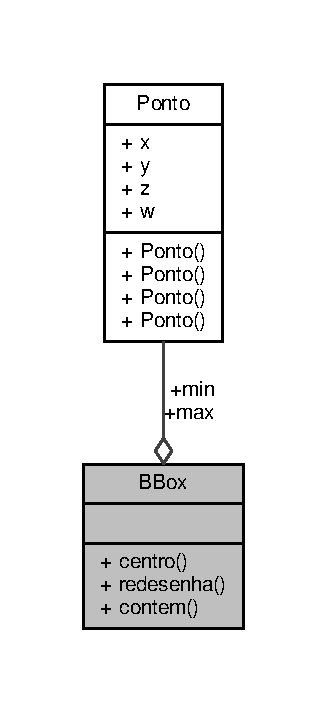
\includegraphics[width=157pt]{classBBox__coll__graph}
\end{center}
\end{figure}
\subsection*{Public Member Functions}
\begin{DoxyCompactItemize}
\item 
\hyperlink{classPonto}{Ponto} \hyperlink{classBBox_a4aad8901de813b3339be3a1770c45ac0}{centro} () const 
\item 
void \hyperlink{classBBox_a820d32399477f89718bf78a3b7de84ec}{redesenha} (const vector$<$ \hyperlink{classPonto}{Ponto} $>$ \&pontos)
\item 
bool \hyperlink{classBBox_a24fa2b41697cd58987a1113e437772d6}{contem} (const \hyperlink{classPonto}{Ponto} \&ponto) const 
\end{DoxyCompactItemize}
\subsection*{Public Attributes}
\begin{DoxyCompactItemize}
\item 
\hyperlink{classPonto}{Ponto} \hyperlink{classBBox_ab65bac30fa278acb493ac63631ad83e3}{min}
\item 
\hyperlink{classPonto}{Ponto} \hyperlink{classBBox_a2eb4d802aaaf2e65c7a03faa91855081}{max}
\end{DoxyCompactItemize}


\subsection{Detailed Description}
Uma Bounding\+Box usada para delimitar um objeto gáfico. 

\begin{DoxyAuthor}{Author}
Arthur Henrique Eggert 
\end{DoxyAuthor}
\begin{DoxyDate}{Date}
2014-\/09-\/21 
\end{DoxyDate}


\subsection{Member Function Documentation}
\hypertarget{classBBox_a4aad8901de813b3339be3a1770c45ac0}{\index{B\+Box@{B\+Box}!centro@{centro}}
\index{centro@{centro}!B\+Box@{B\+Box}}
\subsubsection[{centro}]{\setlength{\rightskip}{0pt plus 5cm}{\bf Ponto} B\+Box\+::centro (
\begin{DoxyParamCaption}
{}
\end{DoxyParamCaption}
) const}}\label{classBBox_a4aad8901de813b3339be3a1770c45ac0}
O centro da \hyperlink{classBBox}{B\+Box} \hypertarget{classBBox_a24fa2b41697cd58987a1113e437772d6}{\index{B\+Box@{B\+Box}!contem@{contem}}
\index{contem@{contem}!B\+Box@{B\+Box}}
\subsubsection[{contem}]{\setlength{\rightskip}{0pt plus 5cm}bool B\+Box\+::contem (
\begin{DoxyParamCaption}
\item[{const {\bf Ponto} \&}]{ponto}
\end{DoxyParamCaption}
) const}}\label{classBBox_a24fa2b41697cd58987a1113e437772d6}
Checa se o ponto esta dentro da \hyperlink{classBBox}{B\+Box} \hypertarget{classBBox_a820d32399477f89718bf78a3b7de84ec}{\index{B\+Box@{B\+Box}!redesenha@{redesenha}}
\index{redesenha@{redesenha}!B\+Box@{B\+Box}}
\subsubsection[{redesenha}]{\setlength{\rightskip}{0pt plus 5cm}void B\+Box\+::redesenha (
\begin{DoxyParamCaption}
\item[{const vector$<$ {\bf Ponto} $>$ \&}]{pontos}
\end{DoxyParamCaption}
)}}\label{classBBox_a820d32399477f89718bf78a3b7de84ec}
Altera a bbox para que a mesma se ajuste ao pontos passados via parametro 

\subsection{Member Data Documentation}
\hypertarget{classBBox_a2eb4d802aaaf2e65c7a03faa91855081}{\index{B\+Box@{B\+Box}!max@{max}}
\index{max@{max}!B\+Box@{B\+Box}}
\subsubsection[{max}]{\setlength{\rightskip}{0pt plus 5cm}{\bf Ponto} B\+Box\+::max}}\label{classBBox_a2eb4d802aaaf2e65c7a03faa91855081}
\hypertarget{classBBox_ab65bac30fa278acb493ac63631ad83e3}{\index{B\+Box@{B\+Box}!min@{min}}
\index{min@{min}!B\+Box@{B\+Box}}
\subsubsection[{min}]{\setlength{\rightskip}{0pt plus 5cm}{\bf Ponto} B\+Box\+::min}}\label{classBBox_ab65bac30fa278acb493ac63631ad83e3}


The documentation for this class was generated from the following files\+:\begin{DoxyCompactItemize}
\item 
\hyperlink{BBox_8hpp}{B\+Box.\+hpp}\item 
\hyperlink{BBox_8cpp}{B\+Box.\+cpp}\end{DoxyCompactItemize}

\hypertarget{classCamera}{\section{Camera Class Reference}
\label{classCamera}\index{Camera@{Camera}}
}


A camera da cena grafica.  




{\ttfamily \#include $<$Camera.\+hpp$>$}



Collaboration diagram for Camera\+:
\nopagebreak
\begin{figure}[H]
\begin{center}
\leavevmode
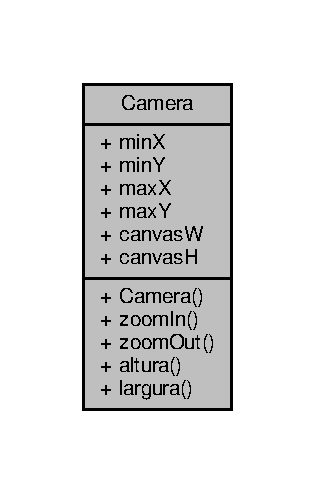
\includegraphics[width=151pt]{classCamera__coll__graph}
\end{center}
\end{figure}
\subsection*{Public Member Functions}
\begin{DoxyCompactItemize}
\item 
\hyperlink{classCamera_a01f94c3543f56ede7af49dc778f19331}{Camera} ()
\item 
void \hyperlink{classCamera_a62d35e87b3eeac9463f43c17b65ef090}{zoom\+In} ()
\item 
void \hyperlink{classCamera_aafc1d985053e11bd553b8a12540a562d}{zoom\+Out} ()
\item 
double \hyperlink{classCamera_a9c26d30741cf690d4f47231d80ccc2e5}{altura} () const 
\item 
double \hyperlink{classCamera_a4dfbaf74d326996e4e725e569f4c2b5b}{largura} () const 
\end{DoxyCompactItemize}
\subsection*{Public Attributes}
\begin{DoxyCompactItemize}
\item 
double \hyperlink{classCamera_a27d1b830bae98aa1641a663535449e58}{min\+X}
\item 
double \hyperlink{classCamera_a3f0be429896f178761bf5849de48026c}{min\+Y}
\item 
double \hyperlink{classCamera_af42e7430e117c722c7aa5cead313f397}{max\+X}
\item 
double \hyperlink{classCamera_ae104c15edb75338f548b1a0a516f90bb}{max\+Y}
\item 
int \hyperlink{classCamera_a6ca24505b375d8d57e6546e914e04d29}{canvas\+W}
\item 
int \hyperlink{classCamera_a2619e7d4b8a7bdb7fc67b51505b0e6a8}{canvas\+H}
\end{DoxyCompactItemize}


\subsection{Detailed Description}
A camera da cena grafica. 

\begin{DoxyAuthor}{Author}
Arthur Henrique Eggert 
\end{DoxyAuthor}
\begin{DoxyDate}{Date}
2014-\/09-\/21 
\end{DoxyDate}


\subsection{Constructor \& Destructor Documentation}
\hypertarget{classCamera_a01f94c3543f56ede7af49dc778f19331}{\index{Camera@{Camera}!Camera@{Camera}}
\index{Camera@{Camera}!Camera@{Camera}}
\subsubsection[{Camera}]{\setlength{\rightskip}{0pt plus 5cm}Camera\+::\+Camera (
\begin{DoxyParamCaption}
{}
\end{DoxyParamCaption}
)}}\label{classCamera_a01f94c3543f56ede7af49dc778f19331}
Cria um novo \hyperlink{classMundo}{Mundo} gráfico 

\subsection{Member Function Documentation}
\hypertarget{classCamera_a9c26d30741cf690d4f47231d80ccc2e5}{\index{Camera@{Camera}!altura@{altura}}
\index{altura@{altura}!Camera@{Camera}}
\subsubsection[{altura}]{\setlength{\rightskip}{0pt plus 5cm}double Camera\+::altura (
\begin{DoxyParamCaption}
{}
\end{DoxyParamCaption}
) const}}\label{classCamera_a9c26d30741cf690d4f47231d80ccc2e5}
A altura do mundo \hypertarget{classCamera_a4dfbaf74d326996e4e725e569f4c2b5b}{\index{Camera@{Camera}!largura@{largura}}
\index{largura@{largura}!Camera@{Camera}}
\subsubsection[{largura}]{\setlength{\rightskip}{0pt plus 5cm}double Camera\+::largura (
\begin{DoxyParamCaption}
{}
\end{DoxyParamCaption}
) const}}\label{classCamera_a4dfbaf74d326996e4e725e569f4c2b5b}
A largura do mundo \hypertarget{classCamera_a62d35e87b3eeac9463f43c17b65ef090}{\index{Camera@{Camera}!zoom\+In@{zoom\+In}}
\index{zoom\+In@{zoom\+In}!Camera@{Camera}}
\subsubsection[{zoom\+In}]{\setlength{\rightskip}{0pt plus 5cm}void Camera\+::zoom\+In (
\begin{DoxyParamCaption}
{}
\end{DoxyParamCaption}
)}}\label{classCamera_a62d35e87b3eeac9463f43c17b65ef090}
Aplica o zoom\+In na camera \hypertarget{classCamera_aafc1d985053e11bd553b8a12540a562d}{\index{Camera@{Camera}!zoom\+Out@{zoom\+Out}}
\index{zoom\+Out@{zoom\+Out}!Camera@{Camera}}
\subsubsection[{zoom\+Out}]{\setlength{\rightskip}{0pt plus 5cm}void Camera\+::zoom\+Out (
\begin{DoxyParamCaption}
{}
\end{DoxyParamCaption}
)}}\label{classCamera_aafc1d985053e11bd553b8a12540a562d}
Aplica o zoom\+Out na camera 

\subsection{Member Data Documentation}
\hypertarget{classCamera_a2619e7d4b8a7bdb7fc67b51505b0e6a8}{\index{Camera@{Camera}!canvas\+H@{canvas\+H}}
\index{canvas\+H@{canvas\+H}!Camera@{Camera}}
\subsubsection[{canvas\+H}]{\setlength{\rightskip}{0pt plus 5cm}int Camera\+::canvas\+H}}\label{classCamera_a2619e7d4b8a7bdb7fc67b51505b0e6a8}
\hypertarget{classCamera_a6ca24505b375d8d57e6546e914e04d29}{\index{Camera@{Camera}!canvas\+W@{canvas\+W}}
\index{canvas\+W@{canvas\+W}!Camera@{Camera}}
\subsubsection[{canvas\+W}]{\setlength{\rightskip}{0pt plus 5cm}int Camera\+::canvas\+W}}\label{classCamera_a6ca24505b375d8d57e6546e914e04d29}
\hypertarget{classCamera_af42e7430e117c722c7aa5cead313f397}{\index{Camera@{Camera}!max\+X@{max\+X}}
\index{max\+X@{max\+X}!Camera@{Camera}}
\subsubsection[{max\+X}]{\setlength{\rightskip}{0pt plus 5cm}double Camera\+::max\+X}}\label{classCamera_af42e7430e117c722c7aa5cead313f397}
\hypertarget{classCamera_ae104c15edb75338f548b1a0a516f90bb}{\index{Camera@{Camera}!max\+Y@{max\+Y}}
\index{max\+Y@{max\+Y}!Camera@{Camera}}
\subsubsection[{max\+Y}]{\setlength{\rightskip}{0pt plus 5cm}double Camera\+::max\+Y}}\label{classCamera_ae104c15edb75338f548b1a0a516f90bb}
\hypertarget{classCamera_a27d1b830bae98aa1641a663535449e58}{\index{Camera@{Camera}!min\+X@{min\+X}}
\index{min\+X@{min\+X}!Camera@{Camera}}
\subsubsection[{min\+X}]{\setlength{\rightskip}{0pt plus 5cm}double Camera\+::min\+X}}\label{classCamera_a27d1b830bae98aa1641a663535449e58}
\hypertarget{classCamera_a3f0be429896f178761bf5849de48026c}{\index{Camera@{Camera}!min\+Y@{min\+Y}}
\index{min\+Y@{min\+Y}!Camera@{Camera}}
\subsubsection[{min\+Y}]{\setlength{\rightskip}{0pt plus 5cm}double Camera\+::min\+Y}}\label{classCamera_a3f0be429896f178761bf5849de48026c}


The documentation for this class was generated from the following files\+:\begin{DoxyCompactItemize}
\item 
\hyperlink{Camera_8hpp}{Camera.\+hpp}\item 
\hyperlink{Camera_8cpp}{Camera.\+cpp}\end{DoxyCompactItemize}

\hypertarget{classCor}{\section{Cor Class Reference}
\label{classCor}\index{Cor@{Cor}}
}


Uma cor R\+G\+B.  




{\ttfamily \#include $<$Cor.\+hpp$>$}



Collaboration diagram for Cor\+:
\nopagebreak
\begin{figure}[H]
\begin{center}
\leavevmode
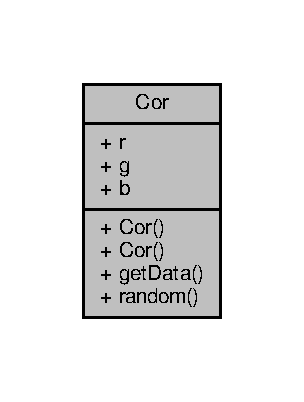
\includegraphics[width=146pt]{classCor__coll__graph}
\end{center}
\end{figure}
\subsection*{Public Member Functions}
\begin{DoxyCompactItemize}
\item 
\hyperlink{classCor_a864fd08c946de50a77cc8b6fd4e7480b}{Cor} ()
\item 
\hyperlink{classCor_ab6e8df5590c8ff0499ce288660a8d3f8}{Cor} (float \hyperlink{classCor_ab7667e786c55c67493b7adfdaae5b44f}{r}, float \hyperlink{classCor_ac6f619ac3749ad997a1c039257ee344e}{g}, float \hyperlink{classCor_a66f9d828b3579b52c88183db73f41f28}{b})
\item 
const float $\ast$ \hyperlink{classCor_aab820fa51901e8088ed072a68ae60ec9}{get\+Data} () const 
\end{DoxyCompactItemize}
\subsection*{Static Public Member Functions}
\begin{DoxyCompactItemize}
\item 
static \hyperlink{classCor}{Cor} \hyperlink{classCor_aec6564749cadce061c6b3e02c066e2ef}{random} ()
\end{DoxyCompactItemize}
\subsection*{Public Attributes}
\begin{DoxyCompactItemize}
\item 
float \hyperlink{classCor_ab7667e786c55c67493b7adfdaae5b44f}{r}
\item 
float \hyperlink{classCor_ac6f619ac3749ad997a1c039257ee344e}{g}
\item 
float \hyperlink{classCor_a66f9d828b3579b52c88183db73f41f28}{b}
\end{DoxyCompactItemize}


\subsection{Detailed Description}
Uma cor R\+G\+B. 

\begin{DoxyAuthor}{Author}
Arthur Henrique Eggert 
\end{DoxyAuthor}
\begin{DoxyDate}{Date}
2014-\/09-\/21
\end{DoxyDate}
Representa um cor R\+G\+B 

\subsection{Constructor \& Destructor Documentation}
\hypertarget{classCor_a864fd08c946de50a77cc8b6fd4e7480b}{\index{Cor@{Cor}!Cor@{Cor}}
\index{Cor@{Cor}!Cor@{Cor}}
\subsubsection[{Cor}]{\setlength{\rightskip}{0pt plus 5cm}Cor\+::\+Cor (
\begin{DoxyParamCaption}
{}
\end{DoxyParamCaption}
)}}\label{classCor_a864fd08c946de50a77cc8b6fd4e7480b}
Cria um objeto de \hyperlink{classCor}{Cor} (0,0,0 -\/ Preto) \hypertarget{classCor_ab6e8df5590c8ff0499ce288660a8d3f8}{\index{Cor@{Cor}!Cor@{Cor}}
\index{Cor@{Cor}!Cor@{Cor}}
\subsubsection[{Cor}]{\setlength{\rightskip}{0pt plus 5cm}Cor\+::\+Cor (
\begin{DoxyParamCaption}
\item[{float}]{r, }
\item[{float}]{g, }
\item[{float}]{b}
\end{DoxyParamCaption}
)}}\label{classCor_ab6e8df5590c8ff0499ce288660a8d3f8}
Cria um objeto com com os valores passados 

\subsection{Member Function Documentation}
\hypertarget{classCor_aab820fa51901e8088ed072a68ae60ec9}{\index{Cor@{Cor}!get\+Data@{get\+Data}}
\index{get\+Data@{get\+Data}!Cor@{Cor}}
\subsubsection[{get\+Data}]{\setlength{\rightskip}{0pt plus 5cm}const float $\ast$ Cor\+::get\+Data (
\begin{DoxyParamCaption}
{}
\end{DoxyParamCaption}
) const}}\label{classCor_aab820fa51901e8088ed072a68ae60ec9}
Retona as cores em um array de float \hypertarget{classCor_aec6564749cadce061c6b3e02c066e2ef}{\index{Cor@{Cor}!random@{random}}
\index{random@{random}!Cor@{Cor}}
\subsubsection[{random}]{\setlength{\rightskip}{0pt plus 5cm}{\bf Cor} Cor\+::random (
\begin{DoxyParamCaption}
{}
\end{DoxyParamCaption}
)\hspace{0.3cm}{\ttfamily [static]}}}\label{classCor_aec6564749cadce061c6b3e02c066e2ef}
Cria um cor randomica. 

\subsection{Member Data Documentation}
\hypertarget{classCor_a66f9d828b3579b52c88183db73f41f28}{\index{Cor@{Cor}!b@{b}}
\index{b@{b}!Cor@{Cor}}
\subsubsection[{b}]{\setlength{\rightskip}{0pt plus 5cm}float Cor\+::b}}\label{classCor_a66f9d828b3579b52c88183db73f41f28}
\hypertarget{classCor_ac6f619ac3749ad997a1c039257ee344e}{\index{Cor@{Cor}!g@{g}}
\index{g@{g}!Cor@{Cor}}
\subsubsection[{g}]{\setlength{\rightskip}{0pt plus 5cm}float Cor\+::g}}\label{classCor_ac6f619ac3749ad997a1c039257ee344e}
\hypertarget{classCor_ab7667e786c55c67493b7adfdaae5b44f}{\index{Cor@{Cor}!r@{r}}
\index{r@{r}!Cor@{Cor}}
\subsubsection[{r}]{\setlength{\rightskip}{0pt plus 5cm}float Cor\+::r}}\label{classCor_ab7667e786c55c67493b7adfdaae5b44f}


The documentation for this class was generated from the following files\+:\begin{DoxyCompactItemize}
\item 
\hyperlink{Cor_8hpp}{Cor.\+hpp}\item 
\hyperlink{Cor_8cpp}{Cor.\+cpp}\end{DoxyCompactItemize}

\hypertarget{classEdicaoCallback}{\section{Edicao\+Callback Class Reference}
\label{classEdicaoCallback}\index{Edicao\+Callback@{Edicao\+Callback}}
}


Estado da aplicação com relação aos momentos de edição.  




{\ttfamily \#include $<$Edicao\+Callback.\+hpp$>$}



Inheritance diagram for Edicao\+Callback\+:
\nopagebreak
\begin{figure}[H]
\begin{center}
\leavevmode
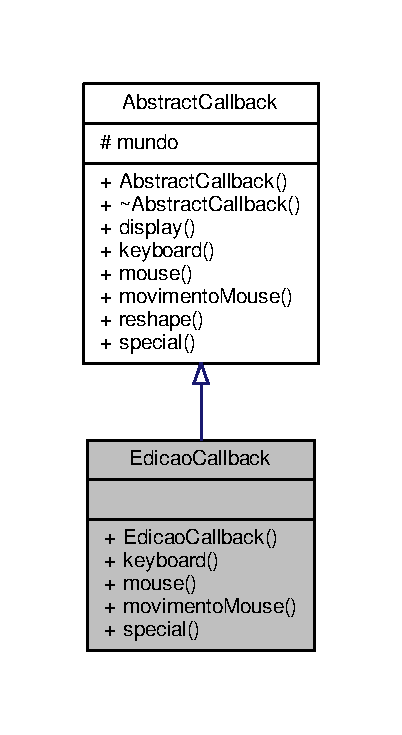
\includegraphics[width=193pt]{classEdicaoCallback__inherit__graph}
\end{center}
\end{figure}


Collaboration diagram for Edicao\+Callback\+:
\nopagebreak
\begin{figure}[H]
\begin{center}
\leavevmode
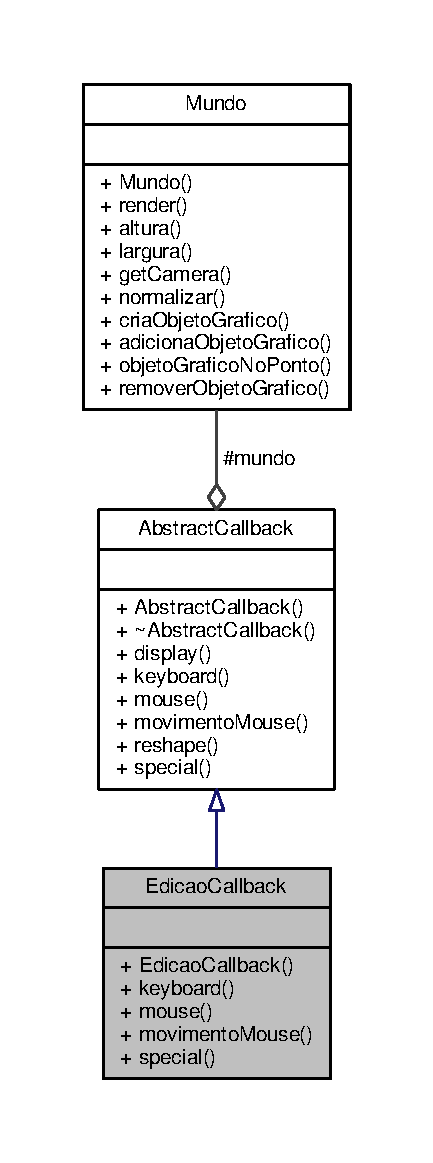
\includegraphics[height=550pt]{classEdicaoCallback__coll__graph}
\end{center}
\end{figure}
\subsection*{Public Member Functions}
\begin{DoxyCompactItemize}
\item 
\hyperlink{classEdicaoCallback_af0564f3f01d1f71793ebf185467a5e6e}{Edicao\+Callback} (\hyperlink{classMundo}{Mundo} \&\hyperlink{classAbstractCallback_a17c2460462c7e985368ef227338d3430}{mundo})
\item 
virtual void \hyperlink{classEdicaoCallback_ab2d6a4a0e971628e460e7505ff289ac9}{keyboard} (unsigned char key, const \hyperlink{classPonto}{Ponto} \&point)
\item 
virtual void \hyperlink{classEdicaoCallback_ad3a885decb234555569dbb3d26f0dcdd}{mouse} (int button, int state, const \hyperlink{classPonto}{Ponto} \&point)
\item 
virtual void \hyperlink{classEdicaoCallback_a58507cc2d8f1e0774fc15aa1d2adca92}{movimento\+Mouse} (const \hyperlink{classPonto}{Ponto} \&point)
\item 
virtual void \hyperlink{classEdicaoCallback_ab3af9b7362efe5d4a8ec18cf840f66c0}{special} (int key, const \hyperlink{classPonto}{Ponto} \&point)
\end{DoxyCompactItemize}
\subsection*{Additional Inherited Members}


\subsection{Detailed Description}
Estado da aplicação com relação aos momentos de edição. 

\begin{DoxyAuthor}{Author}
Arthur Henrique Eggert 
\end{DoxyAuthor}
\begin{DoxyDate}{Date}
2014-\/09-\/21 
\end{DoxyDate}


\subsection{Constructor \& Destructor Documentation}
\hypertarget{classEdicaoCallback_af0564f3f01d1f71793ebf185467a5e6e}{\index{Edicao\+Callback@{Edicao\+Callback}!Edicao\+Callback@{Edicao\+Callback}}
\index{Edicao\+Callback@{Edicao\+Callback}!Edicao\+Callback@{Edicao\+Callback}}
\subsubsection[{Edicao\+Callback}]{\setlength{\rightskip}{0pt plus 5cm}Edicao\+Callback\+::\+Edicao\+Callback (
\begin{DoxyParamCaption}
\item[{{\bf Mundo} \&}]{mundo}
\end{DoxyParamCaption}
)}}\label{classEdicaoCallback_af0564f3f01d1f71793ebf185467a5e6e}


\subsection{Member Function Documentation}
\hypertarget{classEdicaoCallback_ab2d6a4a0e971628e460e7505ff289ac9}{\index{Edicao\+Callback@{Edicao\+Callback}!keyboard@{keyboard}}
\index{keyboard@{keyboard}!Edicao\+Callback@{Edicao\+Callback}}
\subsubsection[{keyboard}]{\setlength{\rightskip}{0pt plus 5cm}void Edicao\+Callback\+::keyboard (
\begin{DoxyParamCaption}
\item[{unsigned char}]{key, }
\item[{const {\bf Ponto} \&}]{point}
\end{DoxyParamCaption}
)\hspace{0.3cm}{\ttfamily [virtual]}}}\label{classEdicaoCallback_ab2d6a4a0e971628e460e7505ff289ac9}
Callback de Teclado 

Reimplemented from \hyperlink{classAbstractCallback_af897d4ee16944785ddb2d90ffad155b2}{Abstract\+Callback}.

\hypertarget{classEdicaoCallback_ad3a885decb234555569dbb3d26f0dcdd}{\index{Edicao\+Callback@{Edicao\+Callback}!mouse@{mouse}}
\index{mouse@{mouse}!Edicao\+Callback@{Edicao\+Callback}}
\subsubsection[{mouse}]{\setlength{\rightskip}{0pt plus 5cm}void Edicao\+Callback\+::mouse (
\begin{DoxyParamCaption}
\item[{int}]{button, }
\item[{int}]{state, }
\item[{const {\bf Ponto} \&}]{point}
\end{DoxyParamCaption}
)\hspace{0.3cm}{\ttfamily [virtual]}}}\label{classEdicaoCallback_ad3a885decb234555569dbb3d26f0dcdd}
Callback de Mouse 

Implements \hyperlink{classAbstractCallback_a1c30a14b8f6212712152364a6620760d}{Abstract\+Callback}.

\hypertarget{classEdicaoCallback_a58507cc2d8f1e0774fc15aa1d2adca92}{\index{Edicao\+Callback@{Edicao\+Callback}!movimento\+Mouse@{movimento\+Mouse}}
\index{movimento\+Mouse@{movimento\+Mouse}!Edicao\+Callback@{Edicao\+Callback}}
\subsubsection[{movimento\+Mouse}]{\setlength{\rightskip}{0pt plus 5cm}void Edicao\+Callback\+::movimento\+Mouse (
\begin{DoxyParamCaption}
\item[{const {\bf Ponto} \&}]{ponto}
\end{DoxyParamCaption}
)\hspace{0.3cm}{\ttfamily [virtual]}}}\label{classEdicaoCallback_a58507cc2d8f1e0774fc15aa1d2adca92}
Callback do movimento de mouse 

Implements \hyperlink{classAbstractCallback_a6a13a67f479eb87c0416d1464b8ef37a}{Abstract\+Callback}.

\hypertarget{classEdicaoCallback_ab3af9b7362efe5d4a8ec18cf840f66c0}{\index{Edicao\+Callback@{Edicao\+Callback}!special@{special}}
\index{special@{special}!Edicao\+Callback@{Edicao\+Callback}}
\subsubsection[{special}]{\setlength{\rightskip}{0pt plus 5cm}void Edicao\+Callback\+::special (
\begin{DoxyParamCaption}
\item[{int}]{key, }
\item[{const {\bf Ponto} \&}]{point}
\end{DoxyParamCaption}
)\hspace{0.3cm}{\ttfamily [virtual]}}}\label{classEdicaoCallback_ab3af9b7362efe5d4a8ec18cf840f66c0}
Calbback para teclas especias do teclado 

Implements \hyperlink{classAbstractCallback_a92270c46a72e1b36f8ad72a26f7c37dd}{Abstract\+Callback}.



The documentation for this class was generated from the following files\+:\begin{DoxyCompactItemize}
\item 
\hyperlink{EdicaoCallback_8hpp}{Edicao\+Callback.\+hpp}\item 
\hyperlink{EdicaoCallback_8cpp}{Edicao\+Callback.\+cpp}\end{DoxyCompactItemize}

\hypertarget{classMundo}{\section{Mundo Class Reference}
\label{classMundo}\index{Mundo@{Mundo}}
}


O Universo gráfico.  




{\ttfamily \#include $<$Mundo.\+hpp$>$}



Collaboration diagram for Mundo\+:
\nopagebreak
\begin{figure}[H]
\begin{center}
\leavevmode
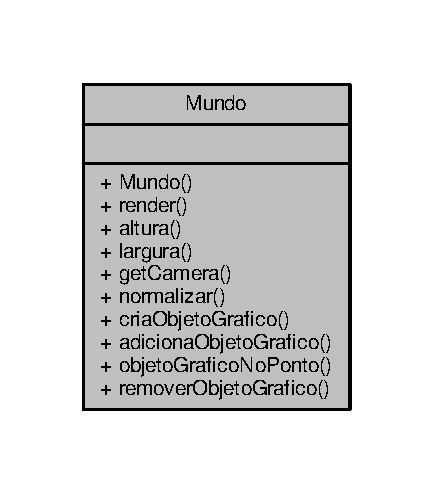
\includegraphics[width=208pt]{classMundo__coll__graph}
\end{center}
\end{figure}
\subsection*{Public Member Functions}
\begin{DoxyCompactItemize}
\item 
\hyperlink{classMundo_a425850071a4ead0edef44ffaa4e3d7d2}{Mundo} ()
\item 
void \hyperlink{classMundo_a1e5d427d26485ab7814cc559a3ae284d}{render} () const 
\item 
double \hyperlink{classMundo_a26788af3ad1edca991d40da2a6f2d577}{altura} () const 
\item 
double \hyperlink{classMundo_a384c4f3106d56abe23d08a6f267c076b}{largura} () const 
\item 
\hyperlink{classCamera}{Camera} \hyperlink{classMundo_ac89e4194871a994e169fb8dd32a191ed}{get\+Camera} ()
\item 
\hyperlink{classPonto}{Ponto} \hyperlink{classMundo_a20150531525b091d689b8f2fc1dd7cea}{normalizar} (int x, int y)
\item 
\hyperlink{classObjetoGrafico}{Objeto\+Grafico} $\ast$ \hyperlink{classMundo_a1d1dfa3384700b11fdbf34593f4e2115}{cria\+Objeto\+Grafico} ()
\item 
void \hyperlink{classMundo_aba8c427fe37a6b3ad82a95b726ce5a0c}{adiciona\+Objeto\+Grafico} ()
\item 
\hyperlink{classObjetoGrafico}{Objeto\+Grafico} $\ast$ \hyperlink{classMundo_a1c7df34ed7eee918781cdc956c199504}{objeto\+Grafico\+No\+Ponto} (const \hyperlink{classPonto}{Ponto} \&ponto)
\item 
void \hyperlink{classMundo_a63d93b69710062da89a50817952e77e4}{remover\+Objeto\+Grafico} (const \hyperlink{classObjetoGrafico}{Objeto\+Grafico} \&object)
\end{DoxyCompactItemize}


\subsection{Detailed Description}
O Universo gráfico. 

\begin{DoxyAuthor}{Author}
Arthur Henrique Eggert 
\end{DoxyAuthor}
\begin{DoxyDate}{Date}
2014-\/09-\/21
\end{DoxyDate}
O \hyperlink{classMundo}{Mundo} ou Universo Gráfico, mantem as informações sobre todos os Objetos\+Graficos e sobre a \hyperlink{classCamera}{Camera} 

\subsection{Constructor \& Destructor Documentation}
\hypertarget{classMundo_a425850071a4ead0edef44ffaa4e3d7d2}{\index{Mundo@{Mundo}!Mundo@{Mundo}}
\index{Mundo@{Mundo}!Mundo@{Mundo}}
\subsubsection[{Mundo}]{\setlength{\rightskip}{0pt plus 5cm}Mundo\+::\+Mundo (
\begin{DoxyParamCaption}
{}
\end{DoxyParamCaption}
)}}\label{classMundo_a425850071a4ead0edef44ffaa4e3d7d2}
Cria um novo \hyperlink{classMundo}{Mundo} gráfico 

\subsection{Member Function Documentation}
\hypertarget{classMundo_aba8c427fe37a6b3ad82a95b726ce5a0c}{\index{Mundo@{Mundo}!adiciona\+Objeto\+Grafico@{adiciona\+Objeto\+Grafico}}
\index{adiciona\+Objeto\+Grafico@{adiciona\+Objeto\+Grafico}!Mundo@{Mundo}}
\subsubsection[{adiciona\+Objeto\+Grafico}]{\setlength{\rightskip}{0pt plus 5cm}void Mundo\+::adiciona\+Objeto\+Grafico (
\begin{DoxyParamCaption}
{}
\end{DoxyParamCaption}
)}}\label{classMundo_aba8c427fe37a6b3ad82a95b726ce5a0c}
Adiciona o rascunho a lista de objetos graficos \hypertarget{classMundo_a26788af3ad1edca991d40da2a6f2d577}{\index{Mundo@{Mundo}!altura@{altura}}
\index{altura@{altura}!Mundo@{Mundo}}
\subsubsection[{altura}]{\setlength{\rightskip}{0pt plus 5cm}double Mundo\+::altura (
\begin{DoxyParamCaption}
{}
\end{DoxyParamCaption}
) const}}\label{classMundo_a26788af3ad1edca991d40da2a6f2d577}
A altura do mundo \hypertarget{classMundo_a1d1dfa3384700b11fdbf34593f4e2115}{\index{Mundo@{Mundo}!cria\+Objeto\+Grafico@{cria\+Objeto\+Grafico}}
\index{cria\+Objeto\+Grafico@{cria\+Objeto\+Grafico}!Mundo@{Mundo}}
\subsubsection[{cria\+Objeto\+Grafico}]{\setlength{\rightskip}{0pt plus 5cm}{\bf Objeto\+Grafico} $\ast$ Mundo\+::cria\+Objeto\+Grafico (
\begin{DoxyParamCaption}
{}
\end{DoxyParamCaption}
)}}\label{classMundo_a1d1dfa3384700b11fdbf34593f4e2115}
Cria um novo rascunho de \hyperlink{classObjetoGrafico}{Objeto\+Grafico} e retorna o mesmo. \hypertarget{classMundo_ac89e4194871a994e169fb8dd32a191ed}{\index{Mundo@{Mundo}!get\+Camera@{get\+Camera}}
\index{get\+Camera@{get\+Camera}!Mundo@{Mundo}}
\subsubsection[{get\+Camera}]{\setlength{\rightskip}{0pt plus 5cm}{\bf Camera} Mundo\+::get\+Camera (
\begin{DoxyParamCaption}
{}
\end{DoxyParamCaption}
)}}\label{classMundo_ac89e4194871a994e169fb8dd32a191ed}
Retona a camera do mundo \hypertarget{classMundo_a384c4f3106d56abe23d08a6f267c076b}{\index{Mundo@{Mundo}!largura@{largura}}
\index{largura@{largura}!Mundo@{Mundo}}
\subsubsection[{largura}]{\setlength{\rightskip}{0pt plus 5cm}double Mundo\+::largura (
\begin{DoxyParamCaption}
{}
\end{DoxyParamCaption}
) const}}\label{classMundo_a384c4f3106d56abe23d08a6f267c076b}
A largura do mundo \hypertarget{classMundo_a20150531525b091d689b8f2fc1dd7cea}{\index{Mundo@{Mundo}!normalizar@{normalizar}}
\index{normalizar@{normalizar}!Mundo@{Mundo}}
\subsubsection[{normalizar}]{\setlength{\rightskip}{0pt plus 5cm}{\bf Ponto} Mundo\+::normalizar (
\begin{DoxyParamCaption}
\item[{int}]{x, }
\item[{int}]{y}
\end{DoxyParamCaption}
)}}\label{classMundo_a20150531525b091d689b8f2fc1dd7cea}
Normaliza um ponto de acordo com o tamanho da tela e o zoom da camera. \hypertarget{classMundo_a1c7df34ed7eee918781cdc956c199504}{\index{Mundo@{Mundo}!objeto\+Grafico\+No\+Ponto@{objeto\+Grafico\+No\+Ponto}}
\index{objeto\+Grafico\+No\+Ponto@{objeto\+Grafico\+No\+Ponto}!Mundo@{Mundo}}
\subsubsection[{objeto\+Grafico\+No\+Ponto}]{\setlength{\rightskip}{0pt plus 5cm}{\bf Objeto\+Grafico} $\ast$ Mundo\+::objeto\+Grafico\+No\+Ponto (
\begin{DoxyParamCaption}
\item[{const {\bf Ponto} \&}]{ponto}
\end{DoxyParamCaption}
)}}\label{classMundo_a1c7df34ed7eee918781cdc956c199504}
Retorna o objeto grafico sobre um determinado ponto. Pode retorna um nullptr se nenhum objeto estiver selecionado \hypertarget{classMundo_a63d93b69710062da89a50817952e77e4}{\index{Mundo@{Mundo}!remover\+Objeto\+Grafico@{remover\+Objeto\+Grafico}}
\index{remover\+Objeto\+Grafico@{remover\+Objeto\+Grafico}!Mundo@{Mundo}}
\subsubsection[{remover\+Objeto\+Grafico}]{\setlength{\rightskip}{0pt plus 5cm}void Mundo\+::remover\+Objeto\+Grafico (
\begin{DoxyParamCaption}
\item[{const {\bf Objeto\+Grafico} \&}]{object}
\end{DoxyParamCaption}
)}}\label{classMundo_a63d93b69710062da89a50817952e77e4}
Remove o objeto grafico passado por paramentro \hypertarget{classMundo_a1e5d427d26485ab7814cc559a3ae284d}{\index{Mundo@{Mundo}!render@{render}}
\index{render@{render}!Mundo@{Mundo}}
\subsubsection[{render}]{\setlength{\rightskip}{0pt plus 5cm}void Mundo\+::render (
\begin{DoxyParamCaption}
{}
\end{DoxyParamCaption}
) const}}\label{classMundo_a1e5d427d26485ab7814cc559a3ae284d}
Renderiza todos os objetosgraficos da cena 

The documentation for this class was generated from the following files\+:\begin{DoxyCompactItemize}
\item 
\hyperlink{Mundo_8hpp}{Mundo.\+hpp}\item 
\hyperlink{Mundo_8cpp}{Mundo.\+cpp}\end{DoxyCompactItemize}

\hypertarget{classObjetoGrafico}{\section{Objeto\+Grafico Class Reference}
\label{classObjetoGrafico}\index{Objeto\+Grafico@{Objeto\+Grafico}}
}


Um Objeto Grafico do mundo.  




{\ttfamily \#include $<$Objeto\+Grafico.\+hpp$>$}



Collaboration diagram for Objeto\+Grafico\+:
\nopagebreak
\begin{figure}[H]
\begin{center}
\leavevmode
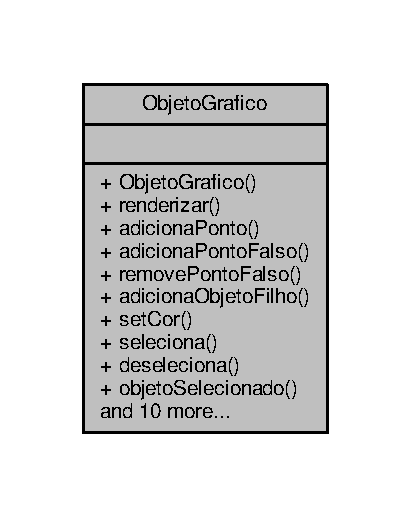
\includegraphics[width=197pt]{classObjetoGrafico__coll__graph}
\end{center}
\end{figure}
\subsection*{Public Member Functions}
\begin{DoxyCompactItemize}
\item 
\hyperlink{classObjetoGrafico_aa9f60661f56d401ea452d1f816baf383}{Objeto\+Grafico} ()
\item 
void \hyperlink{classObjetoGrafico_a5724b1222c13566c383ef45afe509c1d}{renderizar} () const 
\item 
void \hyperlink{classObjetoGrafico_a53501fa66c3e01b16cb3b779ce49b3f2}{adiciona\+Ponto} (const \hyperlink{classPonto}{Ponto} \&ponto)
\item 
void \hyperlink{classObjetoGrafico_ac497e31bacfc78ab649d0141037e2e53}{adiciona\+Ponto\+Falso} (const \hyperlink{classPonto}{Ponto} \&ponto)
\item 
void \hyperlink{classObjetoGrafico_af503f951d52a753e5d585aedfe7a786d}{remove\+Ponto\+Falso} ()
\item 
void \hyperlink{classObjetoGrafico_aa3fe40175c540687c2f5fdc3cfcaaa5e}{adiciona\+Objeto\+Filho} (const \hyperlink{classObjetoGrafico}{Objeto\+Grafico} \&objeto)
\item 
void \hyperlink{classObjetoGrafico_a30c749fe307eb77a071dee9c5afa6901}{set\+Cor} (const \hyperlink{classCor}{Cor} \&cor)
\item 
void \hyperlink{classObjetoGrafico_a3abe25ee87595137e261644901c5433e}{seleciona} ()
\item 
void \hyperlink{classObjetoGrafico_a8fbcf1515b4c000086a0869f883a2649}{deseleciona} ()
\item 
\hyperlink{classObjetoGrafico}{Objeto\+Grafico} $\ast$ \hyperlink{classObjetoGrafico_a0b0e6b4b843662542c4e26237bc13311}{objeto\+Selecionado} ()
\item 
void \hyperlink{classObjetoGrafico_a32858f0dd61d1d4fa2a3450650448b0a}{reseta\+Transformacao} ()
\item 
void \hyperlink{classObjetoGrafico_ae943811015ea3f95985803868de59387}{aplica\+Transformacao} (const \hyperlink{classTransformacao}{Transformacao} \&transformacao)
\item 
void \hyperlink{classObjetoGrafico_a878a53888cfcac3083f02188029f41a6}{muda\+Poligono\+Aberto\+Ou\+Fechado} ()
\item 
void \hyperlink{classObjetoGrafico_a1583cd9219737af248fd81255b388e08}{remove\+Ponto} (const \hyperlink{classPonto}{Ponto} \&ponto)
\item 
void \hyperlink{classObjetoGrafico_aef0874677507e0c6b9937fcce6d99e68}{remove\+Filho} (const \hyperlink{classObjetoGrafico}{Objeto\+Grafico} \&filho)
\item 
\hyperlink{classPonto}{Ponto} $\ast$ \hyperlink{classObjetoGrafico_aa0311d586a8a42b509e7275b803bfe20}{ponto\+Proximo} (const \hyperlink{classPonto}{Ponto} \&ponto)
\item 
void \hyperlink{classObjetoGrafico_a37bea7bf0a47e37db50a7d1c9bf83f4c}{redesenha\+B\+Box} ()
\item 
\hyperlink{classObjetoGrafico}{Objeto\+Grafico} $\ast$ \hyperlink{classObjetoGrafico_a5b64fd5743e6264ad112a274614739c3}{contem} (const \hyperlink{classPonto}{Ponto} \&ponto)
\item 
bool \hyperlink{classObjetoGrafico_aad0037b6a65530597ad19f22b08f4172}{operator==} (const \hyperlink{classObjetoGrafico}{Objeto\+Grafico} \&objeto)
\item 
\hyperlink{classPonto}{Ponto} \hyperlink{classObjetoGrafico_ad3f5691a4da67df86dfcdd8f7c904d47}{centro\+Objeto\+Grafico} () const 
\end{DoxyCompactItemize}


\subsection{Detailed Description}
Um Objeto Grafico do mundo. 

\begin{DoxyAuthor}{Author}
Arthur Henrique Eggert 
\end{DoxyAuthor}
\begin{DoxyDate}{Date}
2014-\/09-\/21
\end{DoxyDate}
Um Objeto Grafico que matem responsabilidade sobre sua cor, filhos, transformação e bbox 

\subsection{Constructor \& Destructor Documentation}
\hypertarget{classObjetoGrafico_aa9f60661f56d401ea452d1f816baf383}{\index{Objeto\+Grafico@{Objeto\+Grafico}!Objeto\+Grafico@{Objeto\+Grafico}}
\index{Objeto\+Grafico@{Objeto\+Grafico}!Objeto\+Grafico@{Objeto\+Grafico}}
\subsubsection[{Objeto\+Grafico}]{\setlength{\rightskip}{0pt plus 5cm}Objeto\+Grafico\+::\+Objeto\+Grafico (
\begin{DoxyParamCaption}
{}
\end{DoxyParamCaption}
)}}\label{classObjetoGrafico_aa9f60661f56d401ea452d1f816baf383}
Cria um novo \hyperlink{classObjetoGrafico}{Objeto\+Grafico} 

\subsection{Member Function Documentation}
\hypertarget{classObjetoGrafico_aa3fe40175c540687c2f5fdc3cfcaaa5e}{\index{Objeto\+Grafico@{Objeto\+Grafico}!adiciona\+Objeto\+Filho@{adiciona\+Objeto\+Filho}}
\index{adiciona\+Objeto\+Filho@{adiciona\+Objeto\+Filho}!Objeto\+Grafico@{Objeto\+Grafico}}
\subsubsection[{adiciona\+Objeto\+Filho}]{\setlength{\rightskip}{0pt plus 5cm}void Objeto\+Grafico\+::adiciona\+Objeto\+Filho (
\begin{DoxyParamCaption}
\item[{const {\bf Objeto\+Grafico} \&}]{objeto}
\end{DoxyParamCaption}
)}}\label{classObjetoGrafico_aa3fe40175c540687c2f5fdc3cfcaaa5e}
Adiciona um obejto filho ao objeto. \hypertarget{classObjetoGrafico_a53501fa66c3e01b16cb3b779ce49b3f2}{\index{Objeto\+Grafico@{Objeto\+Grafico}!adiciona\+Ponto@{adiciona\+Ponto}}
\index{adiciona\+Ponto@{adiciona\+Ponto}!Objeto\+Grafico@{Objeto\+Grafico}}
\subsubsection[{adiciona\+Ponto}]{\setlength{\rightskip}{0pt plus 5cm}void Objeto\+Grafico\+::adiciona\+Ponto (
\begin{DoxyParamCaption}
\item[{const {\bf Ponto} \&}]{ponto}
\end{DoxyParamCaption}
)}}\label{classObjetoGrafico_a53501fa66c3e01b16cb3b779ce49b3f2}
Adiciona um ponto ao objeto \hypertarget{classObjetoGrafico_ac497e31bacfc78ab649d0141037e2e53}{\index{Objeto\+Grafico@{Objeto\+Grafico}!adiciona\+Ponto\+Falso@{adiciona\+Ponto\+Falso}}
\index{adiciona\+Ponto\+Falso@{adiciona\+Ponto\+Falso}!Objeto\+Grafico@{Objeto\+Grafico}}
\subsubsection[{adiciona\+Ponto\+Falso}]{\setlength{\rightskip}{0pt plus 5cm}void Objeto\+Grafico\+::adiciona\+Ponto\+Falso (
\begin{DoxyParamCaption}
\item[{const {\bf Ponto} \&}]{ponto}
\end{DoxyParamCaption}
)}}\label{classObjetoGrafico_ac497e31bacfc78ab649d0141037e2e53}
Adiciona um ponto falso, assim o usuario pode ver o que ocorre ao adicionar este ponto \hypertarget{classObjetoGrafico_ae943811015ea3f95985803868de59387}{\index{Objeto\+Grafico@{Objeto\+Grafico}!aplica\+Transformacao@{aplica\+Transformacao}}
\index{aplica\+Transformacao@{aplica\+Transformacao}!Objeto\+Grafico@{Objeto\+Grafico}}
\subsubsection[{aplica\+Transformacao}]{\setlength{\rightskip}{0pt plus 5cm}void Objeto\+Grafico\+::aplica\+Transformacao (
\begin{DoxyParamCaption}
\item[{const {\bf Transformacao} \&}]{transformacao}
\end{DoxyParamCaption}
)}}\label{classObjetoGrafico_ae943811015ea3f95985803868de59387}
Aplica um trnaformação \hypertarget{classObjetoGrafico_ad3f5691a4da67df86dfcdd8f7c904d47}{\index{Objeto\+Grafico@{Objeto\+Grafico}!centro\+Objeto\+Grafico@{centro\+Objeto\+Grafico}}
\index{centro\+Objeto\+Grafico@{centro\+Objeto\+Grafico}!Objeto\+Grafico@{Objeto\+Grafico}}
\subsubsection[{centro\+Objeto\+Grafico}]{\setlength{\rightskip}{0pt plus 5cm}{\bf Ponto} Objeto\+Grafico\+::centro\+Objeto\+Grafico (
\begin{DoxyParamCaption}
{}
\end{DoxyParamCaption}
) const}}\label{classObjetoGrafico_ad3f5691a4da67df86dfcdd8f7c904d47}
O Centro do objeto grafico \hypertarget{classObjetoGrafico_a5b64fd5743e6264ad112a274614739c3}{\index{Objeto\+Grafico@{Objeto\+Grafico}!contem@{contem}}
\index{contem@{contem}!Objeto\+Grafico@{Objeto\+Grafico}}
\subsubsection[{contem}]{\setlength{\rightskip}{0pt plus 5cm}{\bf Objeto\+Grafico} $\ast$ Objeto\+Grafico\+::contem (
\begin{DoxyParamCaption}
\item[{const {\bf Ponto} \&}]{ponto}
\end{DoxyParamCaption}
)}}\label{classObjetoGrafico_a5b64fd5743e6264ad112a274614739c3}
Verifica se o ponto recebido esta dentro do objeto. \hypertarget{classObjetoGrafico_a8fbcf1515b4c000086a0869f883a2649}{\index{Objeto\+Grafico@{Objeto\+Grafico}!deseleciona@{deseleciona}}
\index{deseleciona@{deseleciona}!Objeto\+Grafico@{Objeto\+Grafico}}
\subsubsection[{deseleciona}]{\setlength{\rightskip}{0pt plus 5cm}void Objeto\+Grafico\+::deseleciona (
\begin{DoxyParamCaption}
{}
\end{DoxyParamCaption}
)}}\label{classObjetoGrafico_a8fbcf1515b4c000086a0869f883a2649}
Deseleciona o Objeto Grafico \hypertarget{classObjetoGrafico_a878a53888cfcac3083f02188029f41a6}{\index{Objeto\+Grafico@{Objeto\+Grafico}!muda\+Poligono\+Aberto\+Ou\+Fechado@{muda\+Poligono\+Aberto\+Ou\+Fechado}}
\index{muda\+Poligono\+Aberto\+Ou\+Fechado@{muda\+Poligono\+Aberto\+Ou\+Fechado}!Objeto\+Grafico@{Objeto\+Grafico}}
\subsubsection[{muda\+Poligono\+Aberto\+Ou\+Fechado}]{\setlength{\rightskip}{0pt plus 5cm}void Objeto\+Grafico\+::muda\+Poligono\+Aberto\+Ou\+Fechado (
\begin{DoxyParamCaption}
{}
\end{DoxyParamCaption}
)}}\label{classObjetoGrafico_a878a53888cfcac3083f02188029f41a6}
Muda a primitiva grafica para identificar um poligono aberto ou fechado \hypertarget{classObjetoGrafico_a0b0e6b4b843662542c4e26237bc13311}{\index{Objeto\+Grafico@{Objeto\+Grafico}!objeto\+Selecionado@{objeto\+Selecionado}}
\index{objeto\+Selecionado@{objeto\+Selecionado}!Objeto\+Grafico@{Objeto\+Grafico}}
\subsubsection[{objeto\+Selecionado}]{\setlength{\rightskip}{0pt plus 5cm}{\bf Objeto\+Grafico} $\ast$ Objeto\+Grafico\+::objeto\+Selecionado (
\begin{DoxyParamCaption}
{}
\end{DoxyParamCaption}
)}}\label{classObjetoGrafico_a0b0e6b4b843662542c4e26237bc13311}
Retorna o objeto selecionado, se ele ou um dos filhos estiver selecionado Retorna nullptr nos demais casos \hypertarget{classObjetoGrafico_aad0037b6a65530597ad19f22b08f4172}{\index{Objeto\+Grafico@{Objeto\+Grafico}!operator==@{operator==}}
\index{operator==@{operator==}!Objeto\+Grafico@{Objeto\+Grafico}}
\subsubsection[{operator==}]{\setlength{\rightskip}{0pt plus 5cm}bool Objeto\+Grafico\+::operator== (
\begin{DoxyParamCaption}
\item[{const {\bf Objeto\+Grafico} \&}]{objeto}
\end{DoxyParamCaption}
)}}\label{classObjetoGrafico_aad0037b6a65530597ad19f22b08f4172}
Compara dois obejtos. \hypertarget{classObjetoGrafico_aa0311d586a8a42b509e7275b803bfe20}{\index{Objeto\+Grafico@{Objeto\+Grafico}!ponto\+Proximo@{ponto\+Proximo}}
\index{ponto\+Proximo@{ponto\+Proximo}!Objeto\+Grafico@{Objeto\+Grafico}}
\subsubsection[{ponto\+Proximo}]{\setlength{\rightskip}{0pt plus 5cm}{\bf Ponto} $\ast$ Objeto\+Grafico\+::ponto\+Proximo (
\begin{DoxyParamCaption}
\item[{const {\bf Ponto} \&}]{ponto}
\end{DoxyParamCaption}
)}}\label{classObjetoGrafico_aa0311d586a8a42b509e7275b803bfe20}
Retorna um ponto proximo ao ponto passado por parametro. \hypertarget{classObjetoGrafico_a37bea7bf0a47e37db50a7d1c9bf83f4c}{\index{Objeto\+Grafico@{Objeto\+Grafico}!redesenha\+B\+Box@{redesenha\+B\+Box}}
\index{redesenha\+B\+Box@{redesenha\+B\+Box}!Objeto\+Grafico@{Objeto\+Grafico}}
\subsubsection[{redesenha\+B\+Box}]{\setlength{\rightskip}{0pt plus 5cm}void Objeto\+Grafico\+::redesenha\+B\+Box (
\begin{DoxyParamCaption}
{}
\end{DoxyParamCaption}
)}}\label{classObjetoGrafico_a37bea7bf0a47e37db50a7d1c9bf83f4c}
Redesenha a \hyperlink{classBBox}{B\+Box} quando um ponto do objeto foi alterado. \hypertarget{classObjetoGrafico_aef0874677507e0c6b9937fcce6d99e68}{\index{Objeto\+Grafico@{Objeto\+Grafico}!remove\+Filho@{remove\+Filho}}
\index{remove\+Filho@{remove\+Filho}!Objeto\+Grafico@{Objeto\+Grafico}}
\subsubsection[{remove\+Filho}]{\setlength{\rightskip}{0pt plus 5cm}void Objeto\+Grafico\+::remove\+Filho (
\begin{DoxyParamCaption}
\item[{const {\bf Objeto\+Grafico} \&}]{filho}
\end{DoxyParamCaption}
)}}\label{classObjetoGrafico_aef0874677507e0c6b9937fcce6d99e68}
Remove o objeto filho igual ao recebido via parametro \hypertarget{classObjetoGrafico_a1583cd9219737af248fd81255b388e08}{\index{Objeto\+Grafico@{Objeto\+Grafico}!remove\+Ponto@{remove\+Ponto}}
\index{remove\+Ponto@{remove\+Ponto}!Objeto\+Grafico@{Objeto\+Grafico}}
\subsubsection[{remove\+Ponto}]{\setlength{\rightskip}{0pt plus 5cm}void Objeto\+Grafico\+::remove\+Ponto (
\begin{DoxyParamCaption}
\item[{const {\bf Ponto} \&}]{ponto}
\end{DoxyParamCaption}
)}}\label{classObjetoGrafico_a1583cd9219737af248fd81255b388e08}
Remove o ponto recebido por paramentro \hypertarget{classObjetoGrafico_af503f951d52a753e5d585aedfe7a786d}{\index{Objeto\+Grafico@{Objeto\+Grafico}!remove\+Ponto\+Falso@{remove\+Ponto\+Falso}}
\index{remove\+Ponto\+Falso@{remove\+Ponto\+Falso}!Objeto\+Grafico@{Objeto\+Grafico}}
\subsubsection[{remove\+Ponto\+Falso}]{\setlength{\rightskip}{0pt plus 5cm}void Objeto\+Grafico\+::remove\+Ponto\+Falso (
\begin{DoxyParamCaption}
{}
\end{DoxyParamCaption}
)}}\label{classObjetoGrafico_af503f951d52a753e5d585aedfe7a786d}
Remove o ultimo ponto falso. \hypertarget{classObjetoGrafico_a5724b1222c13566c383ef45afe509c1d}{\index{Objeto\+Grafico@{Objeto\+Grafico}!renderizar@{renderizar}}
\index{renderizar@{renderizar}!Objeto\+Grafico@{Objeto\+Grafico}}
\subsubsection[{renderizar}]{\setlength{\rightskip}{0pt plus 5cm}void Objeto\+Grafico\+::renderizar (
\begin{DoxyParamCaption}
{}
\end{DoxyParamCaption}
) const}}\label{classObjetoGrafico_a5724b1222c13566c383ef45afe509c1d}
Renderiza o obejto e seus filhos \hypertarget{classObjetoGrafico_a32858f0dd61d1d4fa2a3450650448b0a}{\index{Objeto\+Grafico@{Objeto\+Grafico}!reseta\+Transformacao@{reseta\+Transformacao}}
\index{reseta\+Transformacao@{reseta\+Transformacao}!Objeto\+Grafico@{Objeto\+Grafico}}
\subsubsection[{reseta\+Transformacao}]{\setlength{\rightskip}{0pt plus 5cm}void Objeto\+Grafico\+::reseta\+Transformacao (
\begin{DoxyParamCaption}
{}
\end{DoxyParamCaption}
)}}\label{classObjetoGrafico_a32858f0dd61d1d4fa2a3450650448b0a}
Reseta a matriz de transformação do objeto \hypertarget{classObjetoGrafico_a3abe25ee87595137e261644901c5433e}{\index{Objeto\+Grafico@{Objeto\+Grafico}!seleciona@{seleciona}}
\index{seleciona@{seleciona}!Objeto\+Grafico@{Objeto\+Grafico}}
\subsubsection[{seleciona}]{\setlength{\rightskip}{0pt plus 5cm}void Objeto\+Grafico\+::seleciona (
\begin{DoxyParamCaption}
{}
\end{DoxyParamCaption}
)}}\label{classObjetoGrafico_a3abe25ee87595137e261644901c5433e}
Seta o objeto como selecionado \hypertarget{classObjetoGrafico_a30c749fe307eb77a071dee9c5afa6901}{\index{Objeto\+Grafico@{Objeto\+Grafico}!set\+Cor@{set\+Cor}}
\index{set\+Cor@{set\+Cor}!Objeto\+Grafico@{Objeto\+Grafico}}
\subsubsection[{set\+Cor}]{\setlength{\rightskip}{0pt plus 5cm}void Objeto\+Grafico\+::set\+Cor (
\begin{DoxyParamCaption}
\item[{const {\bf Cor} \&}]{cor}
\end{DoxyParamCaption}
)}}\label{classObjetoGrafico_a30c749fe307eb77a071dee9c5afa6901}
Seta a cor do Objeto Grafico. 

The documentation for this class was generated from the following files\+:\begin{DoxyCompactItemize}
\item 
\hyperlink{ObjetoGrafico_8hpp}{Objeto\+Grafico.\+hpp}\item 
\hyperlink{ObjetoGrafico_8cpp}{Objeto\+Grafico.\+cpp}\end{DoxyCompactItemize}

\hypertarget{classPonto}{\section{Ponto Class Reference}
\label{classPonto}\index{Ponto@{Ponto}}
}


\hyperlink{classPonto}{Ponto} 3\+D.  




{\ttfamily \#include $<$Ponto.\+hpp$>$}



Collaboration diagram for Ponto\+:
\nopagebreak
\begin{figure}[H]
\begin{center}
\leavevmode
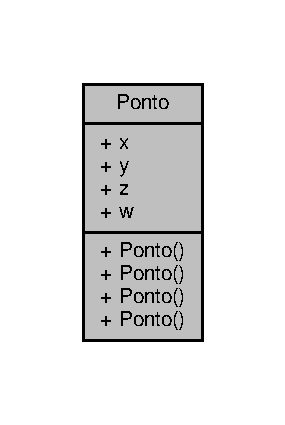
\includegraphics[width=137pt]{classPonto__coll__graph}
\end{center}
\end{figure}
\subsection*{Public Member Functions}
\begin{DoxyCompactItemize}
\item 
\hyperlink{classPonto_a49b03b00e9ebc01c2011c25f6517b93b}{Ponto} ()
\item 
\hyperlink{classPonto_a8f85d65a4e81f86a351cc94612d31add}{Ponto} (double \hyperlink{classPonto_a19d9967c487a947f94938ce37346ed3c}{x}, double \hyperlink{classPonto_afc19597e54764ae43c0211a34adc98c8}{y})
\item 
\hyperlink{classPonto_ad55e3d41b73a92edad7527b07a71d6f0}{Ponto} (double \hyperlink{classPonto_a19d9967c487a947f94938ce37346ed3c}{x}, double \hyperlink{classPonto_afc19597e54764ae43c0211a34adc98c8}{y}, double \hyperlink{classPonto_ab5f76e914355c1bb1c5542a0a6093f5c}{z})
\item 
\hyperlink{classPonto_aec81b7e86a1d6c8cb41690fc0ab54cb4}{Ponto} (double \hyperlink{classPonto_a19d9967c487a947f94938ce37346ed3c}{x}, double \hyperlink{classPonto_afc19597e54764ae43c0211a34adc98c8}{y}, double \hyperlink{classPonto_ab5f76e914355c1bb1c5542a0a6093f5c}{z}, double \hyperlink{classPonto_afb59351a6bdb8509302ffeda9ac77091}{w})
\end{DoxyCompactItemize}
\subsection*{Public Attributes}
\begin{DoxyCompactItemize}
\item 
double \hyperlink{classPonto_a19d9967c487a947f94938ce37346ed3c}{x}
\item 
double \hyperlink{classPonto_afc19597e54764ae43c0211a34adc98c8}{y}
\item 
double \hyperlink{classPonto_ab5f76e914355c1bb1c5542a0a6093f5c}{z}
\item 
double \hyperlink{classPonto_afb59351a6bdb8509302ffeda9ac77091}{w}
\end{DoxyCompactItemize}


\subsection{Detailed Description}
\hyperlink{classPonto}{Ponto} 3\+D. 

\begin{DoxyAuthor}{Author}
Arthur Henrique Eggert 
\end{DoxyAuthor}
\begin{DoxyDate}{Date}
2014-\/09-\/21
\end{DoxyDate}
Representa um ponto com 3 dimensões X, Y e Z, onde Z é sempre 1 

\subsection{Constructor \& Destructor Documentation}
\hypertarget{classPonto_a49b03b00e9ebc01c2011c25f6517b93b}{\index{Ponto@{Ponto}!Ponto@{Ponto}}
\index{Ponto@{Ponto}!Ponto@{Ponto}}
\subsubsection[{Ponto}]{\setlength{\rightskip}{0pt plus 5cm}Ponto\+::\+Ponto (
\begin{DoxyParamCaption}
{}
\end{DoxyParamCaption}
)}}\label{classPonto_a49b03b00e9ebc01c2011c25f6517b93b}
Creates a new point with coordinates (0, 0, 0, 1). \hypertarget{classPonto_a8f85d65a4e81f86a351cc94612d31add}{\index{Ponto@{Ponto}!Ponto@{Ponto}}
\index{Ponto@{Ponto}!Ponto@{Ponto}}
\subsubsection[{Ponto}]{\setlength{\rightskip}{0pt plus 5cm}Ponto\+::\+Ponto (
\begin{DoxyParamCaption}
\item[{double}]{x, }
\item[{double}]{y}
\end{DoxyParamCaption}
)}}\label{classPonto_a8f85d65a4e81f86a351cc94612d31add}
Creates a new point with coordinates (x, y, 0, 1). \hypertarget{classPonto_ad55e3d41b73a92edad7527b07a71d6f0}{\index{Ponto@{Ponto}!Ponto@{Ponto}}
\index{Ponto@{Ponto}!Ponto@{Ponto}}
\subsubsection[{Ponto}]{\setlength{\rightskip}{0pt plus 5cm}Ponto\+::\+Ponto (
\begin{DoxyParamCaption}
\item[{double}]{x, }
\item[{double}]{y, }
\item[{double}]{z}
\end{DoxyParamCaption}
)}}\label{classPonto_ad55e3d41b73a92edad7527b07a71d6f0}
Creates a new point with coordinates (x, y, z, 1). \hypertarget{classPonto_aec81b7e86a1d6c8cb41690fc0ab54cb4}{\index{Ponto@{Ponto}!Ponto@{Ponto}}
\index{Ponto@{Ponto}!Ponto@{Ponto}}
\subsubsection[{Ponto}]{\setlength{\rightskip}{0pt plus 5cm}Ponto\+::\+Ponto (
\begin{DoxyParamCaption}
\item[{double}]{x, }
\item[{double}]{y, }
\item[{double}]{z, }
\item[{double}]{w}
\end{DoxyParamCaption}
)}}\label{classPonto_aec81b7e86a1d6c8cb41690fc0ab54cb4}
Creates a new point with coordinates (x, y, z, w). 

\subsection{Member Data Documentation}
\hypertarget{classPonto_afb59351a6bdb8509302ffeda9ac77091}{\index{Ponto@{Ponto}!w@{w}}
\index{w@{w}!Ponto@{Ponto}}
\subsubsection[{w}]{\setlength{\rightskip}{0pt plus 5cm}double Ponto\+::w}}\label{classPonto_afb59351a6bdb8509302ffeda9ac77091}
\hypertarget{classPonto_a19d9967c487a947f94938ce37346ed3c}{\index{Ponto@{Ponto}!x@{x}}
\index{x@{x}!Ponto@{Ponto}}
\subsubsection[{x}]{\setlength{\rightskip}{0pt plus 5cm}double Ponto\+::x}}\label{classPonto_a19d9967c487a947f94938ce37346ed3c}
\hypertarget{classPonto_afc19597e54764ae43c0211a34adc98c8}{\index{Ponto@{Ponto}!y@{y}}
\index{y@{y}!Ponto@{Ponto}}
\subsubsection[{y}]{\setlength{\rightskip}{0pt plus 5cm}double Ponto\+::y}}\label{classPonto_afc19597e54764ae43c0211a34adc98c8}
\hypertarget{classPonto_ab5f76e914355c1bb1c5542a0a6093f5c}{\index{Ponto@{Ponto}!z@{z}}
\index{z@{z}!Ponto@{Ponto}}
\subsubsection[{z}]{\setlength{\rightskip}{0pt plus 5cm}double Ponto\+::z}}\label{classPonto_ab5f76e914355c1bb1c5542a0a6093f5c}


The documentation for this class was generated from the following files\+:\begin{DoxyCompactItemize}
\item 
\hyperlink{Ponto_8hpp}{Ponto.\+hpp}\item 
\hyperlink{Ponto_8cpp}{Ponto.\+cpp}\end{DoxyCompactItemize}

\hypertarget{classTransformacao}{\section{Transformacao Class Reference}
\label{classTransformacao}\index{Transformacao@{Transformacao}}
}


Uma transformação linear.  




{\ttfamily \#include $<$Transformacao.\+hpp$>$}



Collaboration diagram for Transformacao\+:
\nopagebreak
\begin{figure}[H]
\begin{center}
\leavevmode
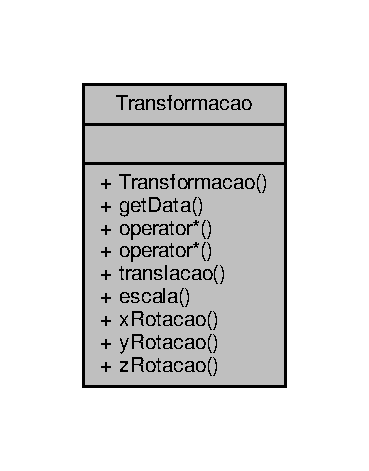
\includegraphics[width=177pt]{classTransformacao__coll__graph}
\end{center}
\end{figure}
\subsection*{Public Member Functions}
\begin{DoxyCompactItemize}
\item 
\hyperlink{classTransformacao_adc00d479b7c2d8d9ef56afe73cb74166}{Transformacao} ()
\item 
const double $\ast$ \hyperlink{classTransformacao_aab2c57d993cf832dd1dff8138dd263d9}{get\+Data} () const 
\item 
\hyperlink{classPonto}{Ponto} \hyperlink{classTransformacao_aadc2790209427a9f25df5b9f27f3ac2e}{operator$\ast$} (const \hyperlink{classPonto}{Ponto} \&ponto) const 
\item 
\hyperlink{classTransformacao}{Transformacao} \hyperlink{classTransformacao_accd6d52cc574f4d564323a84fe0c372a}{operator$\ast$} (const \hyperlink{classTransformacao}{Transformacao} \&rhs) const 
\end{DoxyCompactItemize}
\subsection*{Static Public Member Functions}
\begin{DoxyCompactItemize}
\item 
static \hyperlink{classTransformacao}{Transformacao} \hyperlink{classTransformacao_a1e053f30d9579a5097d44e28de8a2f50}{translacao} (const \hyperlink{classPonto}{Ponto} \&translacao)
\item 
static \hyperlink{classTransformacao}{Transformacao} \hyperlink{classTransformacao_ae8d4d7d168f6dffdfad3f2a4d8ab4139}{escala} (double fator\+De\+X, double fator\+De\+Y, double fator\+De\+Z)
\item 
static \hyperlink{classTransformacao}{Transformacao} \hyperlink{classTransformacao_ab2a54c87392575303f4556abb63ea2b3}{x\+Rotacao} (double rad)
\item 
static \hyperlink{classTransformacao}{Transformacao} \hyperlink{classTransformacao_ae0748337141afe84542995a7e1fb4f1a}{y\+Rotacao} (double rad)
\item 
static \hyperlink{classTransformacao}{Transformacao} \hyperlink{classTransformacao_a3a47b2094d2da2b8c3673defbaa40b2a}{z\+Rotacao} (double rad)
\end{DoxyCompactItemize}


\subsection{Detailed Description}
Uma transformação linear. 

\begin{DoxyAuthor}{Author}
Arthur Henrique Eggert 
\end{DoxyAuthor}
\begin{DoxyDate}{Date}
2014-\/09-\/21
\end{DoxyDate}
Uma transformacao linear usada para transladar, rotacioar ou escalar um objeto grafico. 

\subsection{Constructor \& Destructor Documentation}
\hypertarget{classTransformacao_adc00d479b7c2d8d9ef56afe73cb74166}{\index{Transformacao@{Transformacao}!Transformacao@{Transformacao}}
\index{Transformacao@{Transformacao}!Transformacao@{Transformacao}}
\subsubsection[{Transformacao}]{\setlength{\rightskip}{0pt plus 5cm}Transformacao\+::\+Transformacao (
\begin{DoxyParamCaption}
{}
\end{DoxyParamCaption}
)}}\label{classTransformacao_adc00d479b7c2d8d9ef56afe73cb74166}
Cria uma transformação 

\subsection{Member Function Documentation}
\hypertarget{classTransformacao_ae8d4d7d168f6dffdfad3f2a4d8ab4139}{\index{Transformacao@{Transformacao}!escala@{escala}}
\index{escala@{escala}!Transformacao@{Transformacao}}
\subsubsection[{escala}]{\setlength{\rightskip}{0pt plus 5cm}{\bf Transformacao} Transformacao\+::escala (
\begin{DoxyParamCaption}
\item[{double}]{fator\+De\+X, }
\item[{double}]{fator\+De\+Y, }
\item[{double}]{fator\+De\+Z}
\end{DoxyParamCaption}
)\hspace{0.3cm}{\ttfamily [static]}}}\label{classTransformacao_ae8d4d7d168f6dffdfad3f2a4d8ab4139}

\begin{DoxyItemize}
\item Cria um transformação de escala 
\end{DoxyItemize}\hypertarget{classTransformacao_aab2c57d993cf832dd1dff8138dd263d9}{\index{Transformacao@{Transformacao}!get\+Data@{get\+Data}}
\index{get\+Data@{get\+Data}!Transformacao@{Transformacao}}
\subsubsection[{get\+Data}]{\setlength{\rightskip}{0pt plus 5cm}const double $\ast$ Transformacao\+::get\+Data (
\begin{DoxyParamCaption}
{}
\end{DoxyParamCaption}
) const}}\label{classTransformacao_aab2c57d993cf832dd1dff8138dd263d9}
Retorna os dados da trnaforação como um array de double \hypertarget{classTransformacao_aadc2790209427a9f25df5b9f27f3ac2e}{\index{Transformacao@{Transformacao}!operator$\ast$@{operator$\ast$}}
\index{operator$\ast$@{operator$\ast$}!Transformacao@{Transformacao}}
\subsubsection[{operator$\ast$}]{\setlength{\rightskip}{0pt plus 5cm}{\bf Ponto} Transformacao\+::operator$\ast$ (
\begin{DoxyParamCaption}
\item[{const {\bf Ponto} \&}]{ponto}
\end{DoxyParamCaption}
) const}}\label{classTransformacao_aadc2790209427a9f25df5b9f27f3ac2e}
Aplica a transofmração em um ponto. \hypertarget{classTransformacao_accd6d52cc574f4d564323a84fe0c372a}{\index{Transformacao@{Transformacao}!operator$\ast$@{operator$\ast$}}
\index{operator$\ast$@{operator$\ast$}!Transformacao@{Transformacao}}
\subsubsection[{operator$\ast$}]{\setlength{\rightskip}{0pt plus 5cm}{\bf Transformacao} Transformacao\+::operator$\ast$ (
\begin{DoxyParamCaption}
\item[{const {\bf Transformacao} \&}]{rhs}
\end{DoxyParamCaption}
) const}}\label{classTransformacao_accd6d52cc574f4d564323a84fe0c372a}
Multiplica duas transformações \hypertarget{classTransformacao_a1e053f30d9579a5097d44e28de8a2f50}{\index{Transformacao@{Transformacao}!translacao@{translacao}}
\index{translacao@{translacao}!Transformacao@{Transformacao}}
\subsubsection[{translacao}]{\setlength{\rightskip}{0pt plus 5cm}{\bf Transformacao} Transformacao\+::translacao (
\begin{DoxyParamCaption}
\item[{const {\bf Ponto} \&}]{translacao}
\end{DoxyParamCaption}
)\hspace{0.3cm}{\ttfamily [static]}}}\label{classTransformacao_a1e053f30d9579a5097d44e28de8a2f50}
Cria um transformação de translação \hypertarget{classTransformacao_ab2a54c87392575303f4556abb63ea2b3}{\index{Transformacao@{Transformacao}!x\+Rotacao@{x\+Rotacao}}
\index{x\+Rotacao@{x\+Rotacao}!Transformacao@{Transformacao}}
\subsubsection[{x\+Rotacao}]{\setlength{\rightskip}{0pt plus 5cm}{\bf Transformacao} Transformacao\+::x\+Rotacao (
\begin{DoxyParamCaption}
\item[{double}]{rad}
\end{DoxyParamCaption}
)\hspace{0.3cm}{\ttfamily [static]}}}\label{classTransformacao_ab2a54c87392575303f4556abb63ea2b3}
Cria um transformação de rotaçao no eixo X \hypertarget{classTransformacao_ae0748337141afe84542995a7e1fb4f1a}{\index{Transformacao@{Transformacao}!y\+Rotacao@{y\+Rotacao}}
\index{y\+Rotacao@{y\+Rotacao}!Transformacao@{Transformacao}}
\subsubsection[{y\+Rotacao}]{\setlength{\rightskip}{0pt plus 5cm}{\bf Transformacao} Transformacao\+::y\+Rotacao (
\begin{DoxyParamCaption}
\item[{double}]{rad}
\end{DoxyParamCaption}
)\hspace{0.3cm}{\ttfamily [static]}}}\label{classTransformacao_ae0748337141afe84542995a7e1fb4f1a}
Cria um transformação de rotaçao no eixo Y \hypertarget{classTransformacao_a3a47b2094d2da2b8c3673defbaa40b2a}{\index{Transformacao@{Transformacao}!z\+Rotacao@{z\+Rotacao}}
\index{z\+Rotacao@{z\+Rotacao}!Transformacao@{Transformacao}}
\subsubsection[{z\+Rotacao}]{\setlength{\rightskip}{0pt plus 5cm}{\bf Transformacao} Transformacao\+::z\+Rotacao (
\begin{DoxyParamCaption}
\item[{double}]{rad}
\end{DoxyParamCaption}
)\hspace{0.3cm}{\ttfamily [static]}}}\label{classTransformacao_a3a47b2094d2da2b8c3673defbaa40b2a}
Cria um transformação de rotaçao no eixo Z 

The documentation for this class was generated from the following files\+:\begin{DoxyCompactItemize}
\item 
\hyperlink{Transformacao_8hpp}{Transformacao.\+hpp}\item 
\hyperlink{Transformacao_8cpp}{Transformacao.\+cpp}\end{DoxyCompactItemize}

\chapter{File Documentation}
\hypertarget{AbstractCallback_8cpp}{\section{Abstract\+Callback.\+cpp File Reference}
\label{AbstractCallback_8cpp}\index{Abstract\+Callback.\+cpp@{Abstract\+Callback.\+cpp}}
}
{\ttfamily \#include \char`\"{}Abstract\+Callback.\+hpp\char`\"{}}\\*
{\ttfamily \#include \char`\"{}Ponto.\+hpp\char`\"{}}\\*
{\ttfamily \#include \char`\"{}Mundo.\+hpp\char`\"{}}\\*
{\ttfamily \#include $<$iostream$>$}\\*
Include dependency graph for Abstract\+Callback.\+cpp\+:
\nopagebreak
\begin{figure}[H]
\begin{center}
\leavevmode
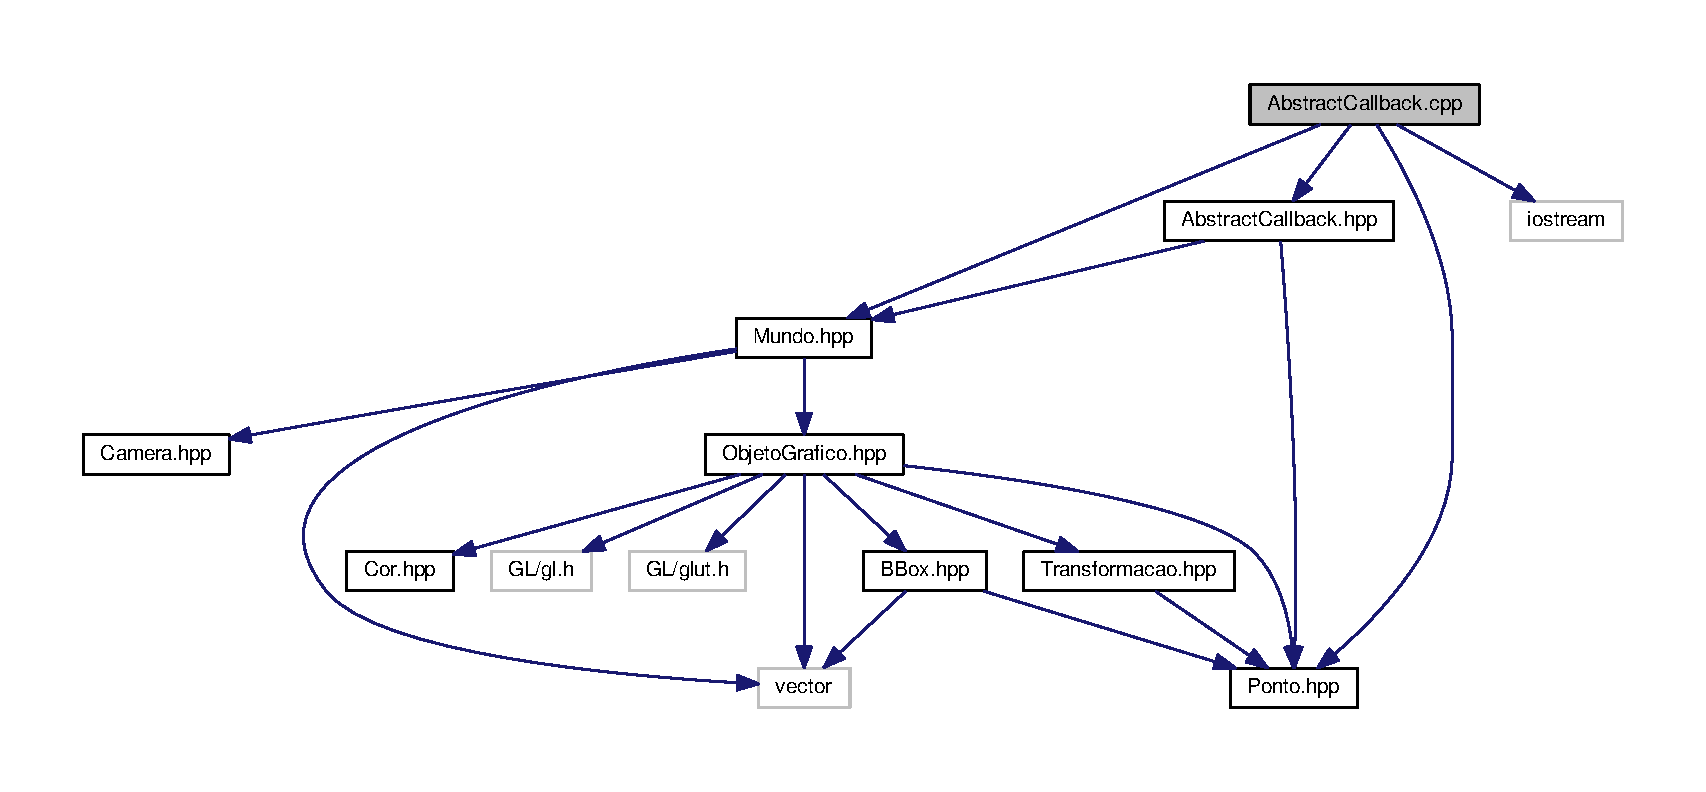
\includegraphics[width=350pt]{AbstractCallback_8cpp__incl}
\end{center}
\end{figure}

\hypertarget{AbstractCallback_8hpp}{\section{Abstract\+Callback.\+hpp File Reference}
\label{AbstractCallback_8hpp}\index{Abstract\+Callback.\+hpp@{Abstract\+Callback.\+hpp}}
}


Definição abstrata da classe da aplicação.  


{\ttfamily \#include \char`\"{}Mundo.\+hpp\char`\"{}}\\*
{\ttfamily \#include \char`\"{}Ponto.\+hpp\char`\"{}}\\*
Include dependency graph for Abstract\+Callback.\+hpp\+:
\nopagebreak
\begin{figure}[H]
\begin{center}
\leavevmode
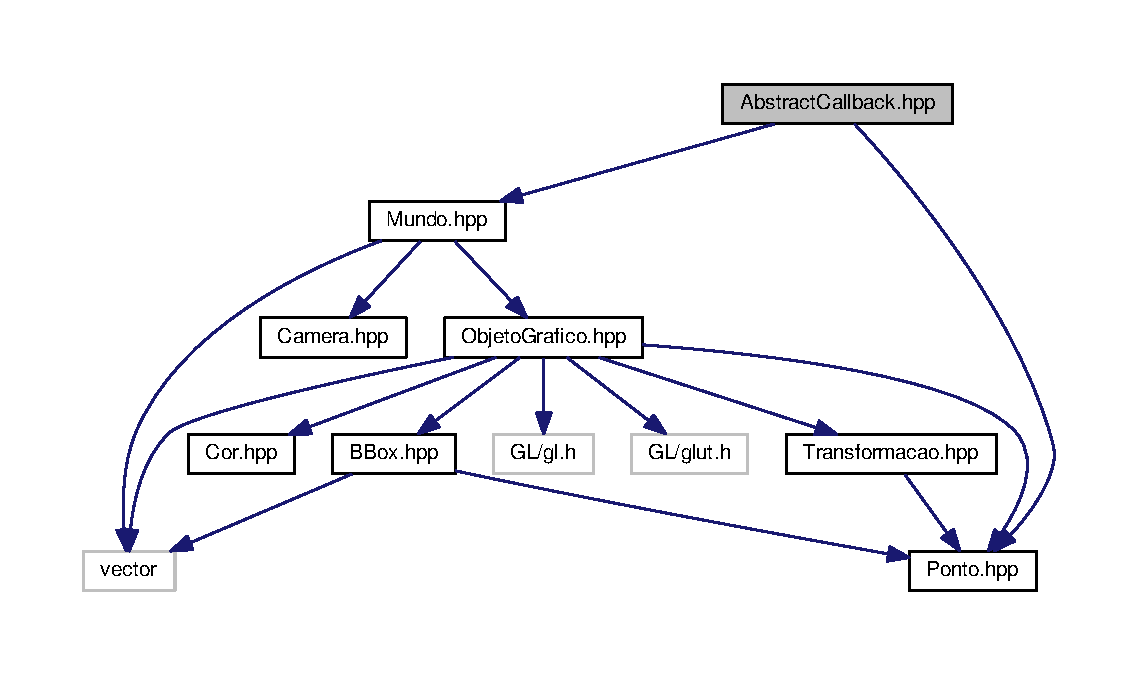
\includegraphics[width=350pt]{AbstractCallback_8hpp__incl}
\end{center}
\end{figure}
This graph shows which files directly or indirectly include this file\+:
\nopagebreak
\begin{figure}[H]
\begin{center}
\leavevmode
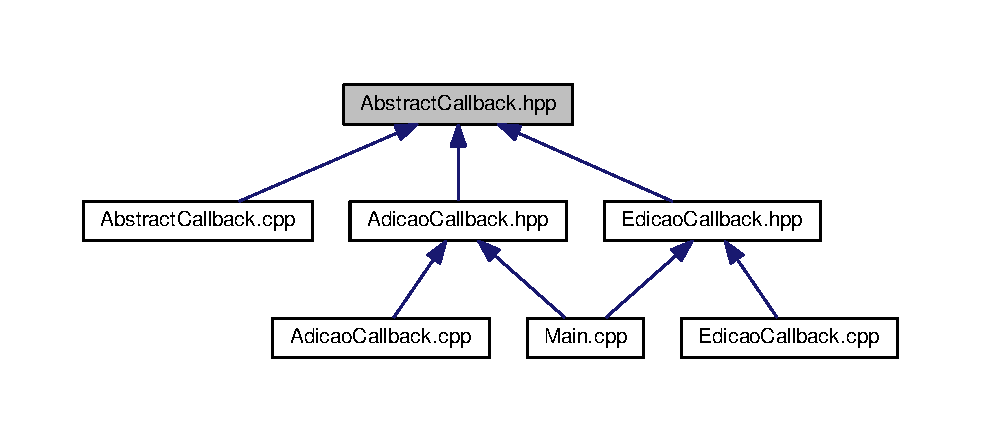
\includegraphics[width=350pt]{AbstractCallback_8hpp__dep__incl}
\end{center}
\end{figure}
\subsection*{Classes}
\begin{DoxyCompactItemize}
\item 
class \hyperlink{classAbstractCallback}{Abstract\+Callback}
\begin{DoxyCompactList}\small\item\em Classe abstrata para lidar com os eventos dependendo do estado. \end{DoxyCompactList}\end{DoxyCompactItemize}


\subsection{Detailed Description}
Definição abstrata da classe da aplicação. 


\begin{DoxyItemize}
\item 
\end{DoxyItemize}
\hypertarget{AdicaoCallback_8cpp}{\section{Adicao\+Callback.\+cpp File Reference}
\label{AdicaoCallback_8cpp}\index{Adicao\+Callback.\+cpp@{Adicao\+Callback.\+cpp}}
}
{\ttfamily \#include \char`\"{}Adicao\+Callback.\+hpp\char`\"{}}\\*
{\ttfamily \#include \char`\"{}Mundo.\+hpp\char`\"{}}\\*
{\ttfamily \#include \char`\"{}Cor.\+hpp\char`\"{}}\\*
{\ttfamily \#include $<$G\+L/gl.\+h$>$}\\*
{\ttfamily \#include $<$G\+L/glut.\+h$>$}\\*
{\ttfamily \#include $<$iostream$>$}\\*
Include dependency graph for Adicao\+Callback.\+cpp\+:
\nopagebreak
\begin{figure}[H]
\begin{center}
\leavevmode
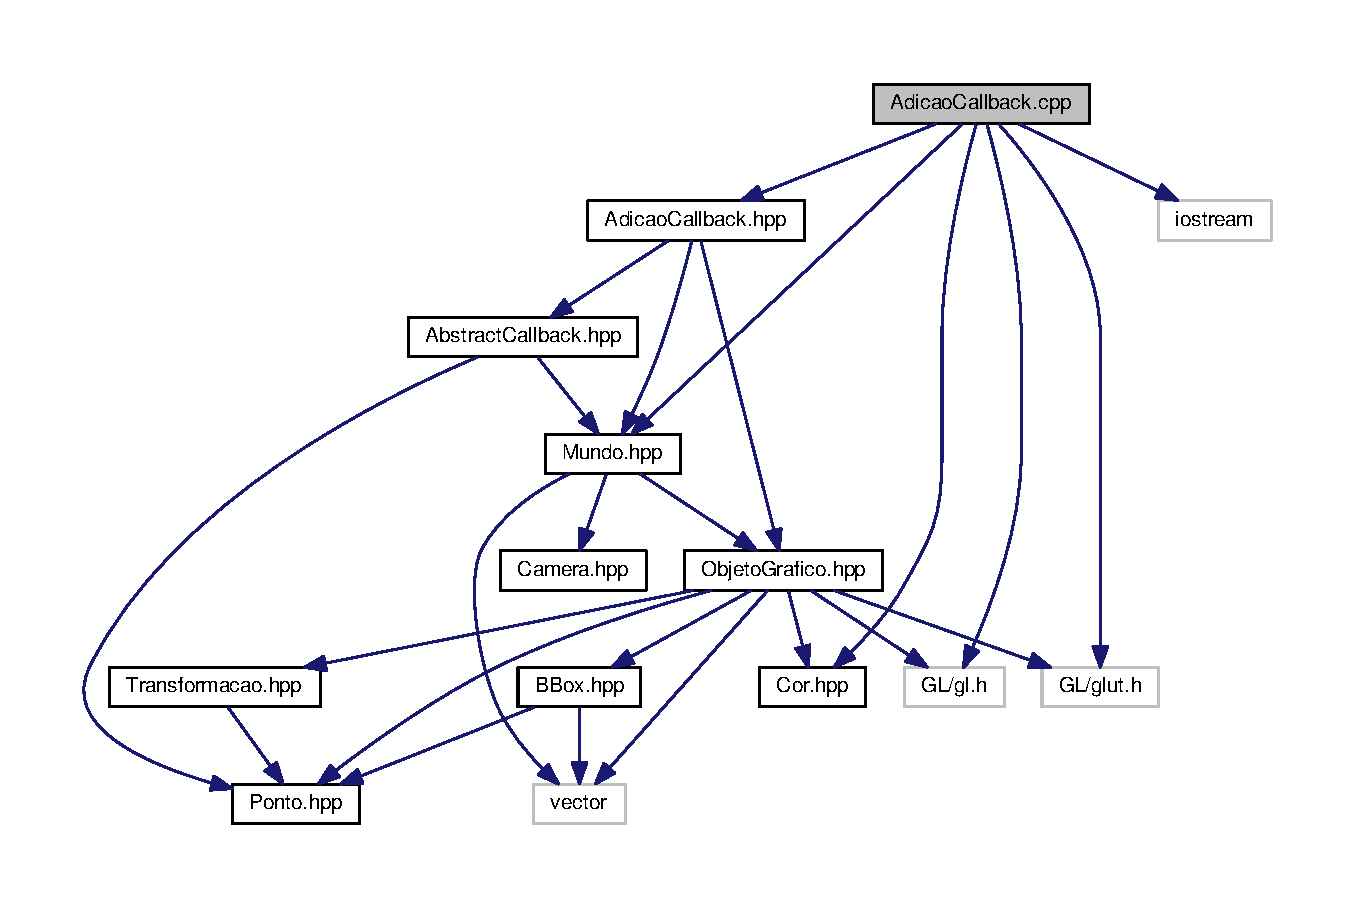
\includegraphics[width=350pt]{AdicaoCallback_8cpp__incl}
\end{center}
\end{figure}

\hypertarget{AdicaoCallback_8hpp}{\section{Adicao\+Callback.\+hpp File Reference}
\label{AdicaoCallback_8hpp}\index{Adicao\+Callback.\+hpp@{Adicao\+Callback.\+hpp}}
}


Definição do estado de adição.  


{\ttfamily \#include \char`\"{}Abstract\+Callback.\+hpp\char`\"{}}\\*
{\ttfamily \#include \char`\"{}Objeto\+Grafico.\+hpp\char`\"{}}\\*
{\ttfamily \#include \char`\"{}Mundo.\+hpp\char`\"{}}\\*
Include dependency graph for Adicao\+Callback.\+hpp\+:
\nopagebreak
\begin{figure}[H]
\begin{center}
\leavevmode
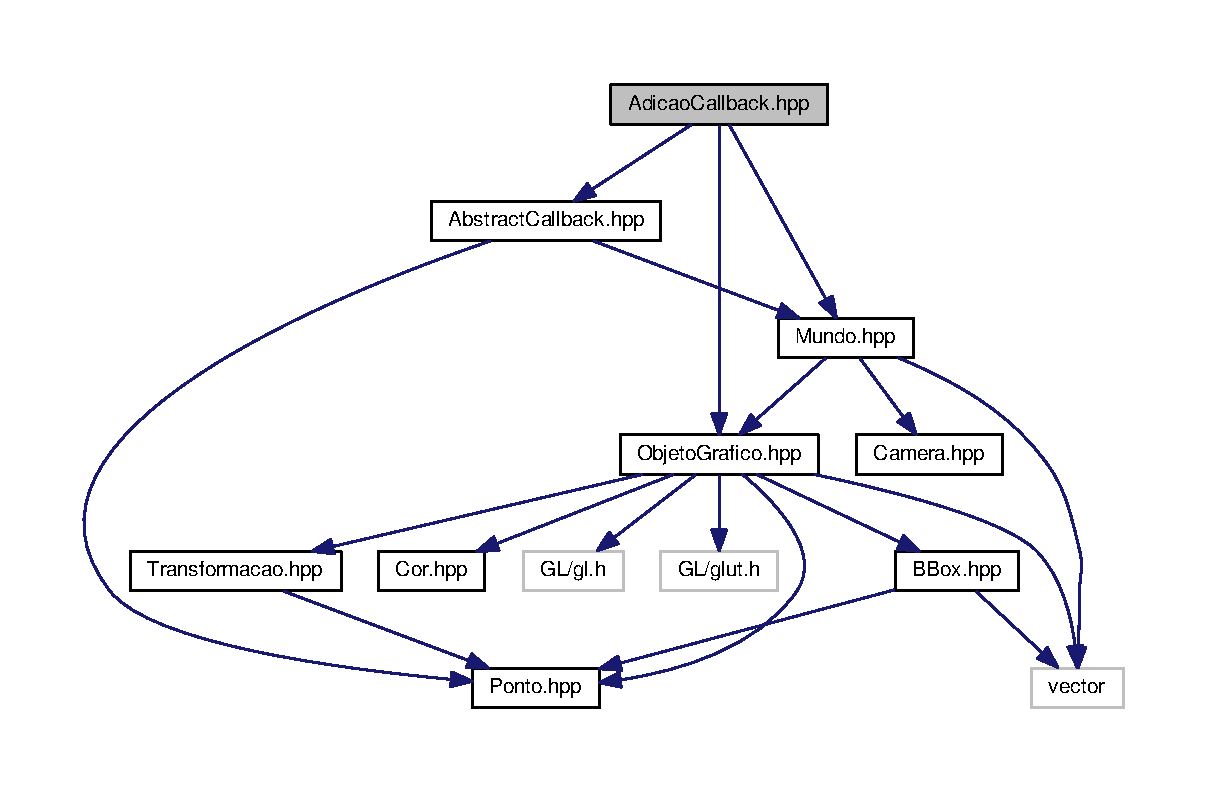
\includegraphics[width=350pt]{AdicaoCallback_8hpp__incl}
\end{center}
\end{figure}
This graph shows which files directly or indirectly include this file\+:
\nopagebreak
\begin{figure}[H]
\begin{center}
\leavevmode
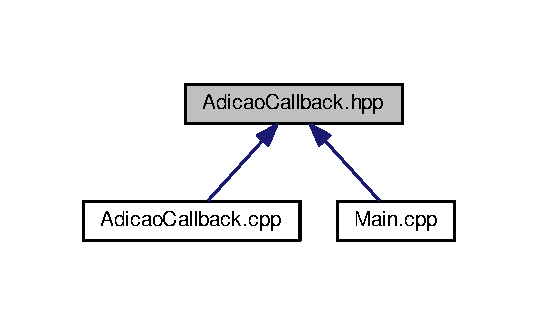
\includegraphics[width=258pt]{AdicaoCallback_8hpp__dep__incl}
\end{center}
\end{figure}
\subsection*{Classes}
\begin{DoxyCompactItemize}
\item 
class \hyperlink{classAdicaoCallback}{Adicao\+Callback}
\begin{DoxyCompactList}\small\item\em Estado da aplicação com relação aos momentos de adição. \end{DoxyCompactList}\end{DoxyCompactItemize}


\subsection{Detailed Description}
Definição do estado de adição. 


\hypertarget{BBox_8cpp}{\section{B\+Box.\+cpp File Reference}
\label{BBox_8cpp}\index{B\+Box.\+cpp@{B\+Box.\+cpp}}
}
{\ttfamily \#include \char`\"{}B\+Box.\+hpp\char`\"{}}\\*
{\ttfamily \#include \char`\"{}Ponto.\+hpp\char`\"{}}\\*
{\ttfamily \#include $<$vector$>$}\\*
Include dependency graph for B\+Box.\+cpp\+:
\nopagebreak
\begin{figure}[H]
\begin{center}
\leavevmode
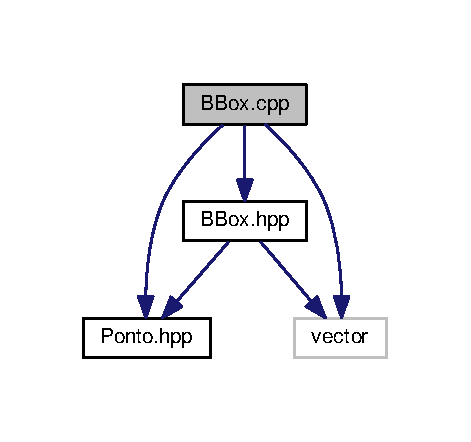
\includegraphics[width=226pt]{BBox_8cpp__incl}
\end{center}
\end{figure}
\subsection*{Functions}
\begin{DoxyCompactItemize}
\item 
bool \hyperlink{BBox_8cpp_a262a0b451e64500a51be1089e68dc514}{operator==} (const \hyperlink{classBBox}{B\+Box} \&lhs, const \hyperlink{classBBox}{B\+Box} \&rhs)
\end{DoxyCompactItemize}


\subsection{Function Documentation}
\hypertarget{BBox_8cpp_a262a0b451e64500a51be1089e68dc514}{\index{B\+Box.\+cpp@{B\+Box.\+cpp}!operator==@{operator==}}
\index{operator==@{operator==}!B\+Box.\+cpp@{B\+Box.\+cpp}}
\subsubsection[{operator==}]{\setlength{\rightskip}{0pt plus 5cm}bool operator== (
\begin{DoxyParamCaption}
\item[{const {\bf B\+Box} \&}]{essa, }
\item[{const {\bf B\+Box} \&}]{outra}
\end{DoxyParamCaption}
)}}\label{BBox_8cpp_a262a0b451e64500a51be1089e68dc514}
Compara 2 \hyperlink{classBBox}{B\+Box}. 
\hypertarget{BBox_8hpp}{\section{B\+Box.\+hpp File Reference}
\label{BBox_8hpp}\index{B\+Box.\+hpp@{B\+Box.\+hpp}}
}


Definição da \hyperlink{classBBox}{B\+Box}.  


{\ttfamily \#include \char`\"{}Ponto.\+hpp\char`\"{}}\\*
{\ttfamily \#include $<$vector$>$}\\*
Include dependency graph for B\+Box.\+hpp\+:
\nopagebreak
\begin{figure}[H]
\begin{center}
\leavevmode
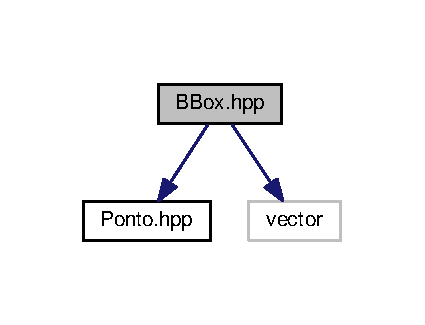
\includegraphics[width=204pt]{BBox_8hpp__incl}
\end{center}
\end{figure}
This graph shows which files directly or indirectly include this file\+:
\nopagebreak
\begin{figure}[H]
\begin{center}
\leavevmode
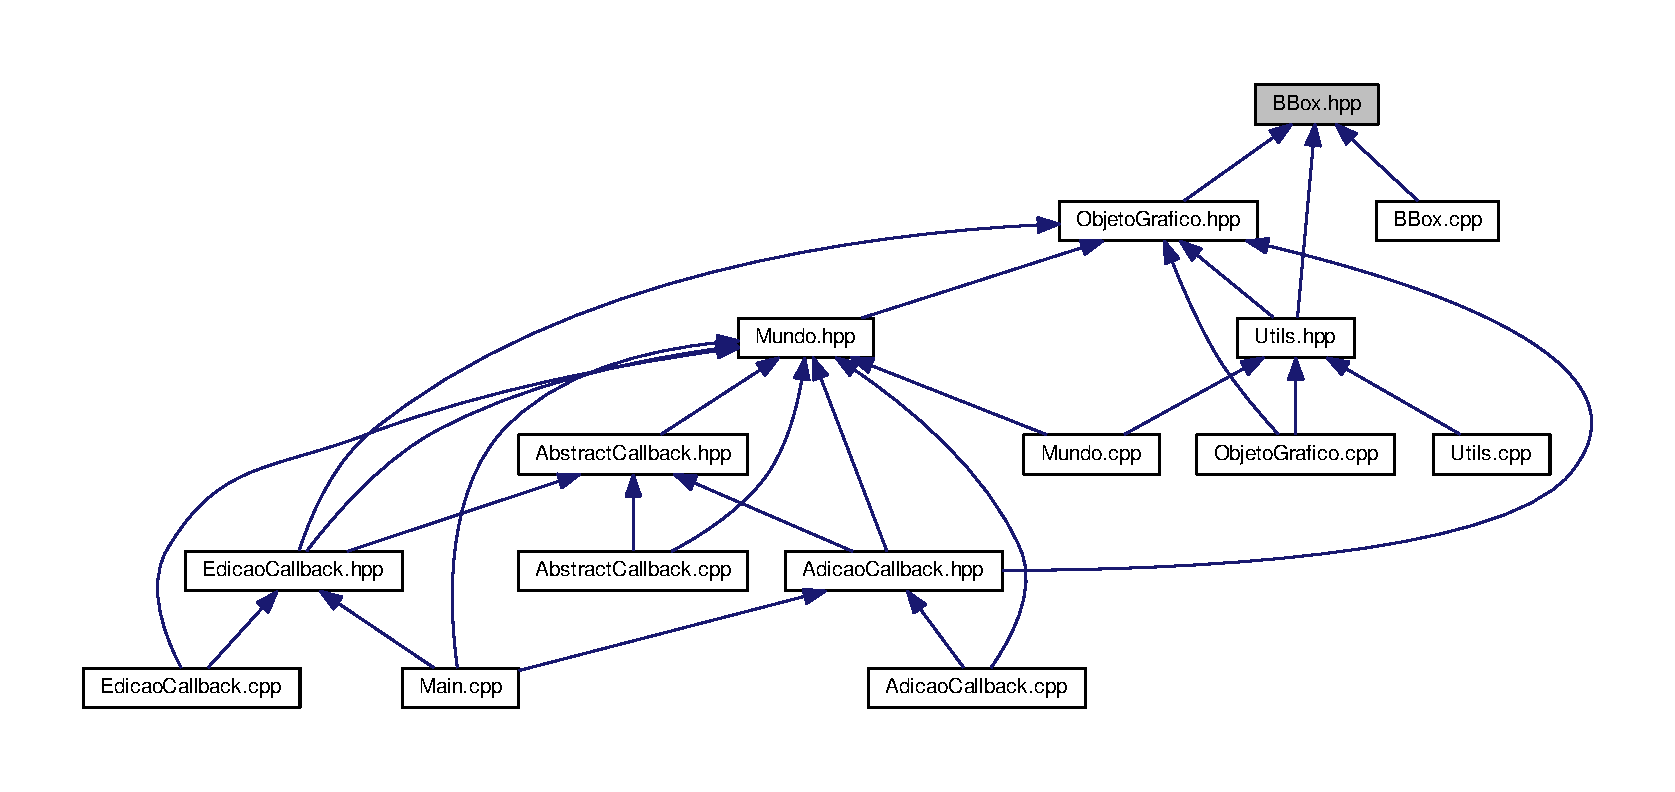
\includegraphics[width=350pt]{BBox_8hpp__dep__incl}
\end{center}
\end{figure}
\subsection*{Classes}
\begin{DoxyCompactItemize}
\item 
class \hyperlink{classBBox}{B\+Box}
\begin{DoxyCompactList}\small\item\em Uma Bounding\+Box usada para delimitar um objeto gáfico. \end{DoxyCompactList}\end{DoxyCompactItemize}
\subsection*{Functions}
\begin{DoxyCompactItemize}
\item 
bool \hyperlink{BBox_8hpp_a0aa8fab2a9731789883541e9bc4242e0}{operator==} (const \hyperlink{classBBox}{B\+Box} \&essa, const \hyperlink{classBBox}{B\+Box} \&outra)
\end{DoxyCompactItemize}


\subsection{Detailed Description}
Definição da \hyperlink{classBBox}{B\+Box}. 



\subsection{Function Documentation}
\hypertarget{BBox_8hpp_a0aa8fab2a9731789883541e9bc4242e0}{\index{B\+Box.\+hpp@{B\+Box.\+hpp}!operator==@{operator==}}
\index{operator==@{operator==}!B\+Box.\+hpp@{B\+Box.\+hpp}}
\subsubsection[{operator==}]{\setlength{\rightskip}{0pt plus 5cm}bool operator== (
\begin{DoxyParamCaption}
\item[{const {\bf B\+Box} \&}]{essa, }
\item[{const {\bf B\+Box} \&}]{outra}
\end{DoxyParamCaption}
)}}\label{BBox_8hpp_a0aa8fab2a9731789883541e9bc4242e0}
Compara 2 \hyperlink{classBBox}{B\+Box}. 
\hypertarget{Camera_8cpp}{\section{Camera.\+cpp File Reference}
\label{Camera_8cpp}\index{Camera.\+cpp@{Camera.\+cpp}}
}
{\ttfamily \#include \char`\"{}Camera.\+hpp\char`\"{}}\\*
Include dependency graph for Camera.\+cpp\+:
\nopagebreak
\begin{figure}[H]
\begin{center}
\leavevmode
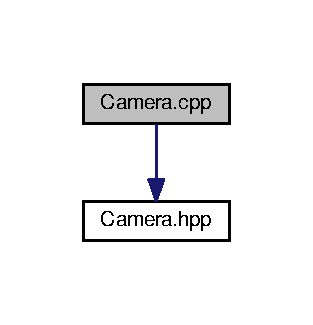
\includegraphics[width=150pt]{Camera_8cpp__incl}
\end{center}
\end{figure}

\hypertarget{Camera_8hpp}{\section{Camera.\+hpp File Reference}
\label{Camera_8hpp}\index{Camera.\+hpp@{Camera.\+hpp}}
}
This graph shows which files directly or indirectly include this file\+:
\nopagebreak
\begin{figure}[H]
\begin{center}
\leavevmode
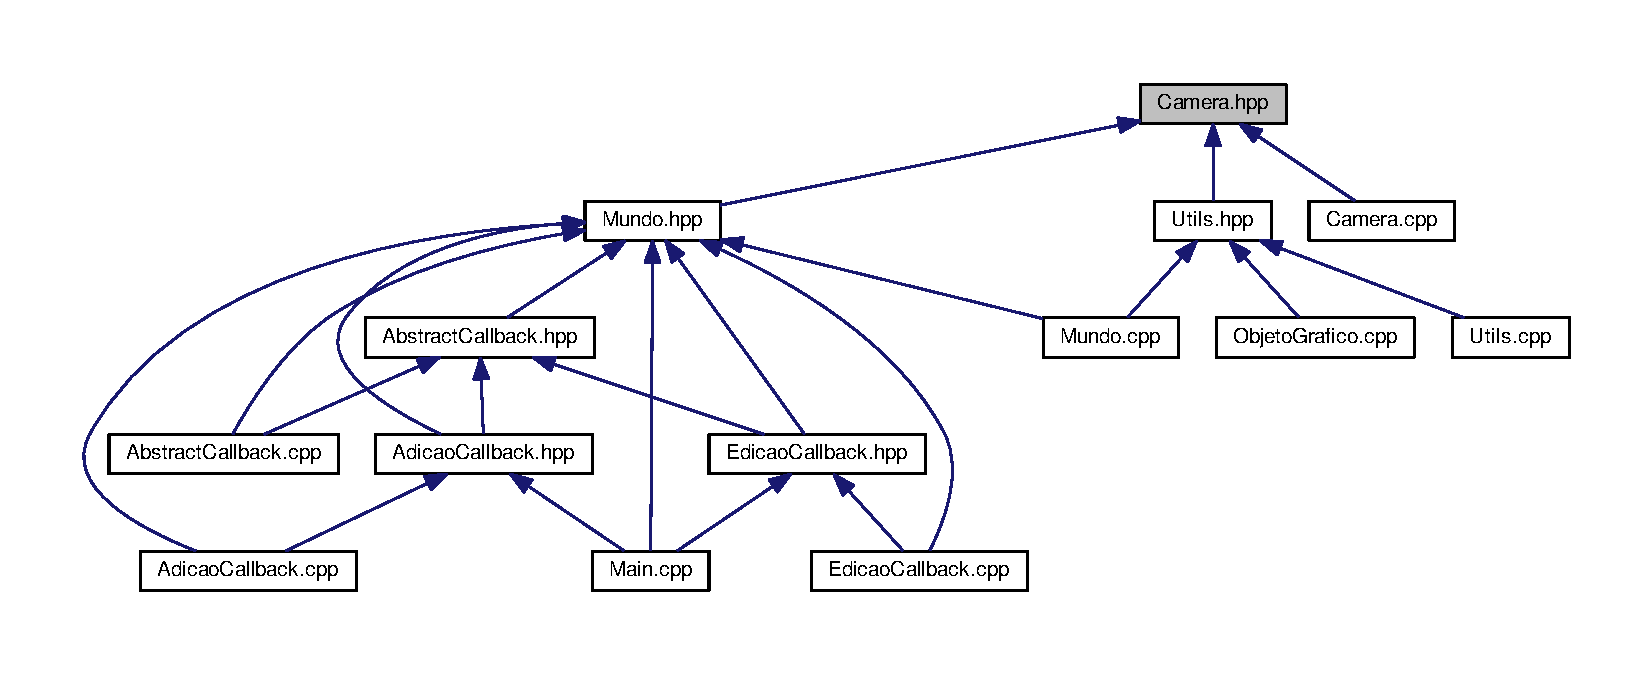
\includegraphics[width=350pt]{Camera_8hpp__dep__incl}
\end{center}
\end{figure}
\subsection*{Classes}
\begin{DoxyCompactItemize}
\item 
class \hyperlink{classCamera}{Camera}
\begin{DoxyCompactList}\small\item\em A camera da cena grafica. \end{DoxyCompactList}\end{DoxyCompactItemize}

\hypertarget{Cor_8cpp}{\section{Cor.\+cpp File Reference}
\label{Cor_8cpp}\index{Cor.\+cpp@{Cor.\+cpp}}
}
{\ttfamily \#include \char`\"{}Cor.\+hpp\char`\"{}}\\*
{\ttfamily \#include $<$random$>$}\\*
{\ttfamily \#include $<$iostream$>$}\\*
Include dependency graph for Cor.\+cpp\+:
\nopagebreak
\begin{figure}[H]
\begin{center}
\leavevmode
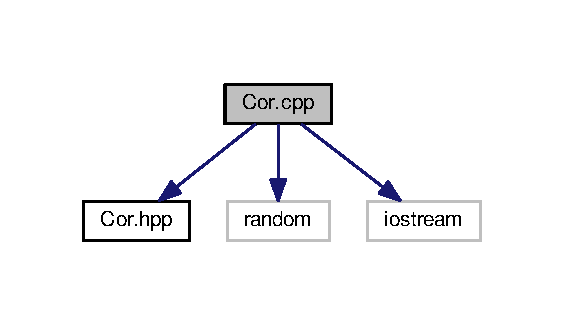
\includegraphics[width=271pt]{Cor_8cpp__incl}
\end{center}
\end{figure}

\hypertarget{Cor_8hpp}{\section{Cor.\+hpp File Reference}
\label{Cor_8hpp}\index{Cor.\+hpp@{Cor.\+hpp}}
}


Definição de \hyperlink{classCamera}{Camera}.  


This graph shows which files directly or indirectly include this file\+:
\nopagebreak
\begin{figure}[H]
\begin{center}
\leavevmode
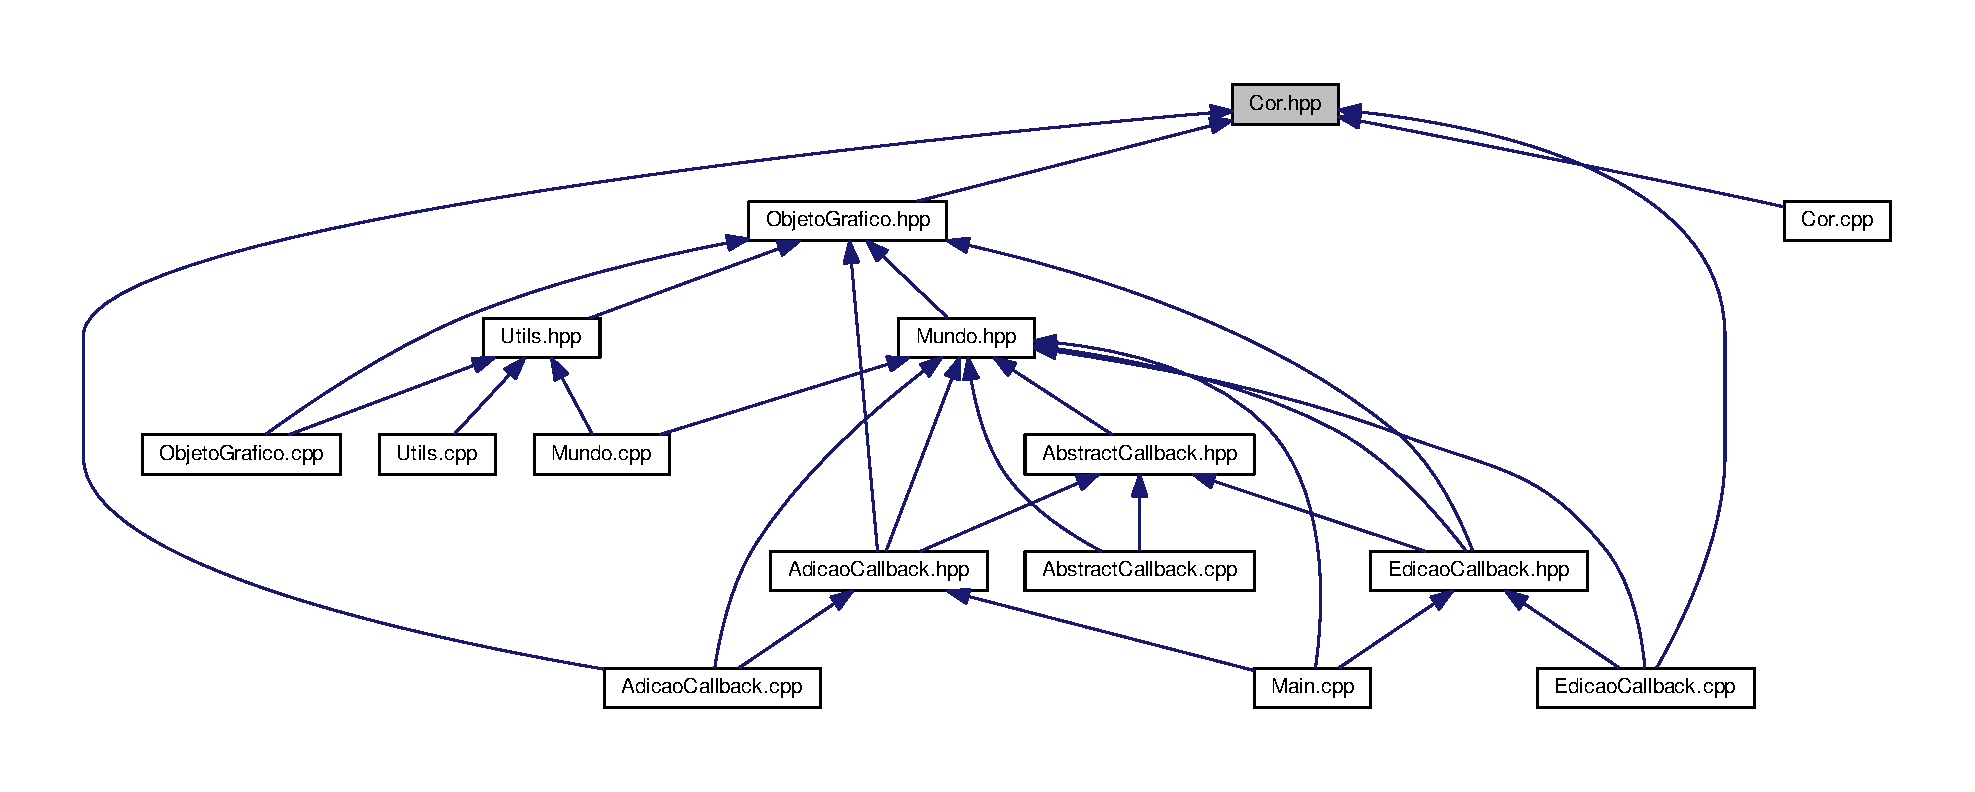
\includegraphics[width=350pt]{Cor_8hpp__dep__incl}
\end{center}
\end{figure}
\subsection*{Classes}
\begin{DoxyCompactItemize}
\item 
class \hyperlink{classCor}{Cor}
\begin{DoxyCompactList}\small\item\em Uma cor R\+G\+B. \end{DoxyCompactList}\end{DoxyCompactItemize}
\subsection*{Variables}
\begin{DoxyCompactItemize}
\item 
const \hyperlink{classCor}{Cor} \hyperlink{Cor_8hpp_abd7af605710473c3b03b9846f5ff439f}{P\+R\+E\+T\+O} (0.\+0f, 0.\+0f, 0.\+0f)
\item 
const \hyperlink{classCor}{Cor} \hyperlink{Cor_8hpp_a0c70b3d200d2d4575587cc155e8ac9c2}{B\+R\+A\+N\+C\+O} (1.\+0f, 1.\+0f, 1.\+0f)
\item 
const \hyperlink{classCor}{Cor} \hyperlink{Cor_8hpp_a664ca4992d0fce115959114e965fe8c3}{V\+E\+R\+M\+E\+L\+H\+O} (1.\+0f, 0.\+0f, 0.\+0f)
\item 
const \hyperlink{classCor}{Cor} \hyperlink{Cor_8hpp_a31ad86e862eca6bc2bed35efa56b3a1b}{V\+E\+R\+D\+E} (0.\+0f, 1.\+0f, 0.\+0f)
\item 
const \hyperlink{classCor}{Cor} \hyperlink{Cor_8hpp_a78d06bb82f952810da0726246599b5d5}{A\+Z\+U\+L} (0.\+0f, 0.\+0f, 1.\+0f)
\item 
const \hyperlink{classCor}{Cor} \hyperlink{Cor_8hpp_a3da43f0a120f015226b99d412c3c7ef0}{A\+M\+A\+R\+E\+L\+O} (1.\+0f, 1.\+0f, 0.\+0f)
\item 
const \hyperlink{classCor}{Cor} \hyperlink{Cor_8hpp_a65d9b54040dc910b3fca1e0c31278a41}{R\+O\+S\+A} (1.\+0f, 0.\+0f, 1.\+0f)
\item 
const \hyperlink{classCor}{Cor} \hyperlink{Cor_8hpp_a3d4fddabbbc9f76bfc7c60bf63c1b44b}{C\+Y\+A\+N} (0.\+0f, 1.\+0f, 1.\+0f)
\end{DoxyCompactItemize}


\subsection{Detailed Description}
Definição de \hyperlink{classCamera}{Camera}. 

Definição de \hyperlink{classCor}{Cor}.

\subsection{Variable Documentation}
\hypertarget{Cor_8hpp_a3da43f0a120f015226b99d412c3c7ef0}{\index{Cor.\+hpp@{Cor.\+hpp}!A\+M\+A\+R\+E\+L\+O@{A\+M\+A\+R\+E\+L\+O}}
\index{A\+M\+A\+R\+E\+L\+O@{A\+M\+A\+R\+E\+L\+O}!Cor.\+hpp@{Cor.\+hpp}}
\subsubsection[{A\+M\+A\+R\+E\+L\+O}]{\setlength{\rightskip}{0pt plus 5cm}const {\bf Cor} A\+M\+A\+R\+E\+L\+O(1.\+0f, 1.\+0f, 0.\+0f)}}\label{Cor_8hpp_a3da43f0a120f015226b99d412c3c7ef0}
\hypertarget{Cor_8hpp_a78d06bb82f952810da0726246599b5d5}{\index{Cor.\+hpp@{Cor.\+hpp}!A\+Z\+U\+L@{A\+Z\+U\+L}}
\index{A\+Z\+U\+L@{A\+Z\+U\+L}!Cor.\+hpp@{Cor.\+hpp}}
\subsubsection[{A\+Z\+U\+L}]{\setlength{\rightskip}{0pt plus 5cm}const {\bf Cor} A\+Z\+U\+L(0.\+0f, 0.\+0f, 1.\+0f)}}\label{Cor_8hpp_a78d06bb82f952810da0726246599b5d5}
\hypertarget{Cor_8hpp_a0c70b3d200d2d4575587cc155e8ac9c2}{\index{Cor.\+hpp@{Cor.\+hpp}!B\+R\+A\+N\+C\+O@{B\+R\+A\+N\+C\+O}}
\index{B\+R\+A\+N\+C\+O@{B\+R\+A\+N\+C\+O}!Cor.\+hpp@{Cor.\+hpp}}
\subsubsection[{B\+R\+A\+N\+C\+O}]{\setlength{\rightskip}{0pt plus 5cm}const {\bf Cor} B\+R\+A\+N\+C\+O(1.\+0f, 1.\+0f, 1.\+0f)}}\label{Cor_8hpp_a0c70b3d200d2d4575587cc155e8ac9c2}
\hypertarget{Cor_8hpp_a3d4fddabbbc9f76bfc7c60bf63c1b44b}{\index{Cor.\+hpp@{Cor.\+hpp}!C\+Y\+A\+N@{C\+Y\+A\+N}}
\index{C\+Y\+A\+N@{C\+Y\+A\+N}!Cor.\+hpp@{Cor.\+hpp}}
\subsubsection[{C\+Y\+A\+N}]{\setlength{\rightskip}{0pt plus 5cm}const {\bf Cor} C\+Y\+A\+N(0.\+0f, 1.\+0f, 1.\+0f)}}\label{Cor_8hpp_a3d4fddabbbc9f76bfc7c60bf63c1b44b}
\hypertarget{Cor_8hpp_abd7af605710473c3b03b9846f5ff439f}{\index{Cor.\+hpp@{Cor.\+hpp}!P\+R\+E\+T\+O@{P\+R\+E\+T\+O}}
\index{P\+R\+E\+T\+O@{P\+R\+E\+T\+O}!Cor.\+hpp@{Cor.\+hpp}}
\subsubsection[{P\+R\+E\+T\+O}]{\setlength{\rightskip}{0pt plus 5cm}const {\bf Cor} P\+R\+E\+T\+O(0.\+0f, 0.\+0f, 0.\+0f)}}\label{Cor_8hpp_abd7af605710473c3b03b9846f5ff439f}
\hypertarget{Cor_8hpp_a65d9b54040dc910b3fca1e0c31278a41}{\index{Cor.\+hpp@{Cor.\+hpp}!R\+O\+S\+A@{R\+O\+S\+A}}
\index{R\+O\+S\+A@{R\+O\+S\+A}!Cor.\+hpp@{Cor.\+hpp}}
\subsubsection[{R\+O\+S\+A}]{\setlength{\rightskip}{0pt plus 5cm}const {\bf Cor} R\+O\+S\+A(1.\+0f, 0.\+0f, 1.\+0f)}}\label{Cor_8hpp_a65d9b54040dc910b3fca1e0c31278a41}
\hypertarget{Cor_8hpp_a31ad86e862eca6bc2bed35efa56b3a1b}{\index{Cor.\+hpp@{Cor.\+hpp}!V\+E\+R\+D\+E@{V\+E\+R\+D\+E}}
\index{V\+E\+R\+D\+E@{V\+E\+R\+D\+E}!Cor.\+hpp@{Cor.\+hpp}}
\subsubsection[{V\+E\+R\+D\+E}]{\setlength{\rightskip}{0pt plus 5cm}const {\bf Cor} V\+E\+R\+D\+E(0.\+0f, 1.\+0f, 0.\+0f)}}\label{Cor_8hpp_a31ad86e862eca6bc2bed35efa56b3a1b}
\hypertarget{Cor_8hpp_a664ca4992d0fce115959114e965fe8c3}{\index{Cor.\+hpp@{Cor.\+hpp}!V\+E\+R\+M\+E\+L\+H\+O@{V\+E\+R\+M\+E\+L\+H\+O}}
\index{V\+E\+R\+M\+E\+L\+H\+O@{V\+E\+R\+M\+E\+L\+H\+O}!Cor.\+hpp@{Cor.\+hpp}}
\subsubsection[{V\+E\+R\+M\+E\+L\+H\+O}]{\setlength{\rightskip}{0pt plus 5cm}const {\bf Cor} V\+E\+R\+M\+E\+L\+H\+O(1.\+0f, 0.\+0f, 0.\+0f)}}\label{Cor_8hpp_a664ca4992d0fce115959114e965fe8c3}

\hypertarget{EdicaoCallback_8cpp}{\section{Edicao\+Callback.\+cpp File Reference}
\label{EdicaoCallback_8cpp}\index{Edicao\+Callback.\+cpp@{Edicao\+Callback.\+cpp}}
}
{\ttfamily \#include \char`\"{}Edicao\+Callback.\+hpp\char`\"{}}\\*
{\ttfamily \#include \char`\"{}Cor.\+hpp\char`\"{}}\\*
{\ttfamily \#include \char`\"{}Mundo.\+hpp\char`\"{}}\\*
Include dependency graph for Edicao\+Callback.\+cpp\+:
\nopagebreak
\begin{figure}[H]
\begin{center}
\leavevmode
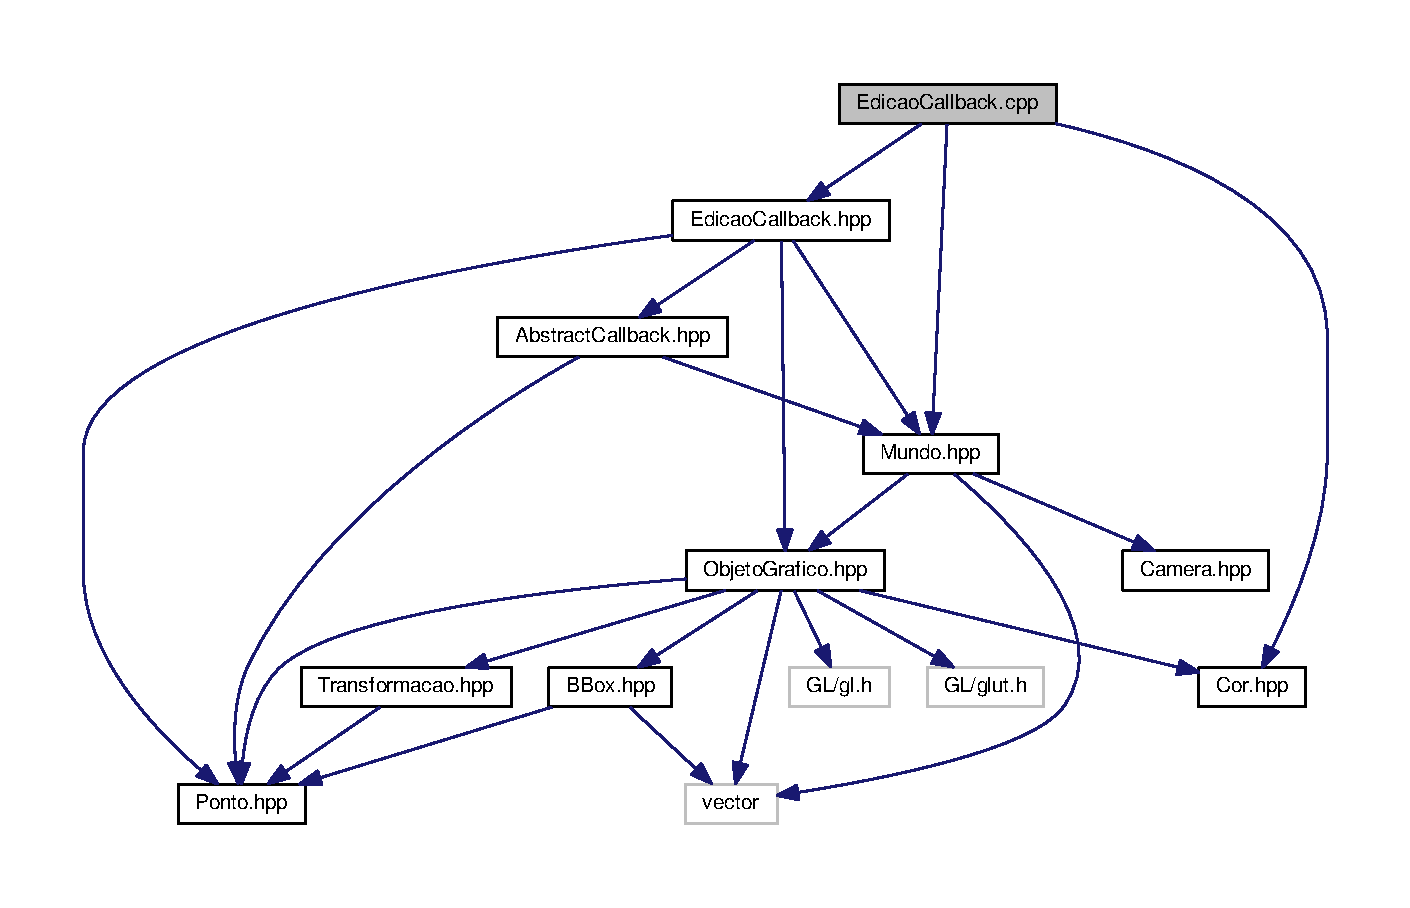
\includegraphics[width=350pt]{EdicaoCallback_8cpp__incl}
\end{center}
\end{figure}
\subsection*{Variables}
\begin{DoxyCompactItemize}
\item 
const double \hyperlink{EdicaoCallback_8cpp_ab2200ad59fd793c5d330782444a18e04}{T\+R\+A\+N\+S\+L\+A\+C\+A\+O} = 2.\+0
\item 
const double \hyperlink{EdicaoCallback_8cpp_aad7e7da69c7d21e2d896509bacc0d10b}{E\+S\+C\+A\+L\+A} = 1.\+1
\item 
const double \hyperlink{EdicaoCallback_8cpp_a4350bac41853f7709b13865c5602a298}{R\+O\+T\+A\+C\+A\+O} = 0.\+1
\end{DoxyCompactItemize}


\subsection{Variable Documentation}
\hypertarget{EdicaoCallback_8cpp_aad7e7da69c7d21e2d896509bacc0d10b}{\index{Edicao\+Callback.\+cpp@{Edicao\+Callback.\+cpp}!E\+S\+C\+A\+L\+A@{E\+S\+C\+A\+L\+A}}
\index{E\+S\+C\+A\+L\+A@{E\+S\+C\+A\+L\+A}!Edicao\+Callback.\+cpp@{Edicao\+Callback.\+cpp}}
\subsubsection[{E\+S\+C\+A\+L\+A}]{\setlength{\rightskip}{0pt plus 5cm}const double E\+S\+C\+A\+L\+A = 1.\+1}}\label{EdicaoCallback_8cpp_aad7e7da69c7d21e2d896509bacc0d10b}
\hypertarget{EdicaoCallback_8cpp_a4350bac41853f7709b13865c5602a298}{\index{Edicao\+Callback.\+cpp@{Edicao\+Callback.\+cpp}!R\+O\+T\+A\+C\+A\+O@{R\+O\+T\+A\+C\+A\+O}}
\index{R\+O\+T\+A\+C\+A\+O@{R\+O\+T\+A\+C\+A\+O}!Edicao\+Callback.\+cpp@{Edicao\+Callback.\+cpp}}
\subsubsection[{R\+O\+T\+A\+C\+A\+O}]{\setlength{\rightskip}{0pt plus 5cm}const double R\+O\+T\+A\+C\+A\+O = 0.\+1}}\label{EdicaoCallback_8cpp_a4350bac41853f7709b13865c5602a298}
\hypertarget{EdicaoCallback_8cpp_ab2200ad59fd793c5d330782444a18e04}{\index{Edicao\+Callback.\+cpp@{Edicao\+Callback.\+cpp}!T\+R\+A\+N\+S\+L\+A\+C\+A\+O@{T\+R\+A\+N\+S\+L\+A\+C\+A\+O}}
\index{T\+R\+A\+N\+S\+L\+A\+C\+A\+O@{T\+R\+A\+N\+S\+L\+A\+C\+A\+O}!Edicao\+Callback.\+cpp@{Edicao\+Callback.\+cpp}}
\subsubsection[{T\+R\+A\+N\+S\+L\+A\+C\+A\+O}]{\setlength{\rightskip}{0pt plus 5cm}const double T\+R\+A\+N\+S\+L\+A\+C\+A\+O = 2.\+0}}\label{EdicaoCallback_8cpp_ab2200ad59fd793c5d330782444a18e04}

\hypertarget{EdicaoCallback_8hpp}{\section{Edicao\+Callback.\+hpp File Reference}
\label{EdicaoCallback_8hpp}\index{Edicao\+Callback.\+hpp@{Edicao\+Callback.\+hpp}}
}


Definição do estado de edição.  


{\ttfamily \#include \char`\"{}Abstract\+Callback.\+hpp\char`\"{}}\\*
{\ttfamily \#include \char`\"{}Objeto\+Grafico.\+hpp\char`\"{}}\\*
{\ttfamily \#include \char`\"{}Mundo.\+hpp\char`\"{}}\\*
{\ttfamily \#include \char`\"{}Ponto.\+hpp\char`\"{}}\\*
Include dependency graph for Edicao\+Callback.\+hpp\+:
\nopagebreak
\begin{figure}[H]
\begin{center}
\leavevmode
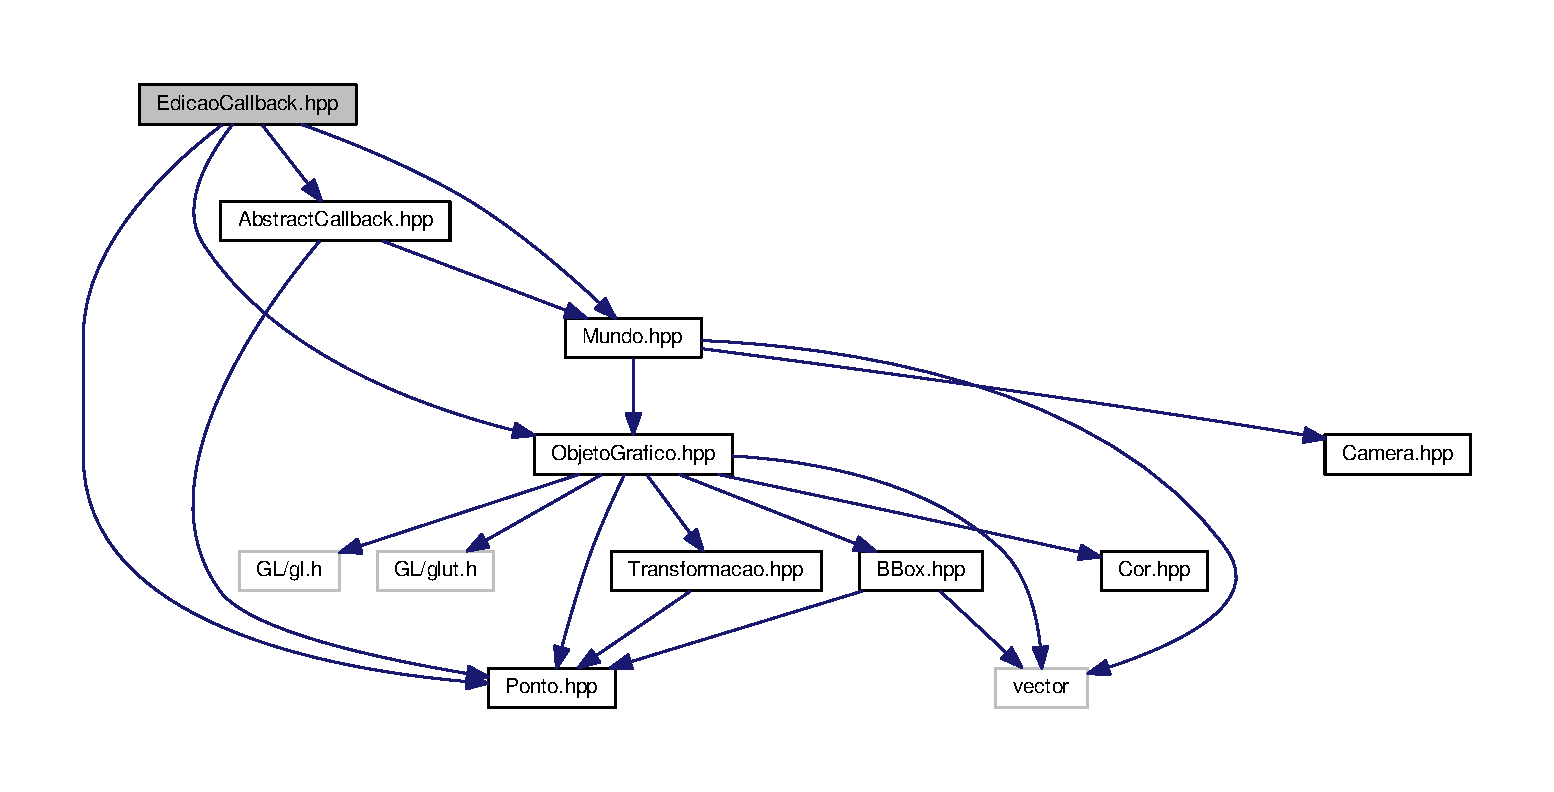
\includegraphics[width=350pt]{EdicaoCallback_8hpp__incl}
\end{center}
\end{figure}
This graph shows which files directly or indirectly include this file\+:
\nopagebreak
\begin{figure}[H]
\begin{center}
\leavevmode
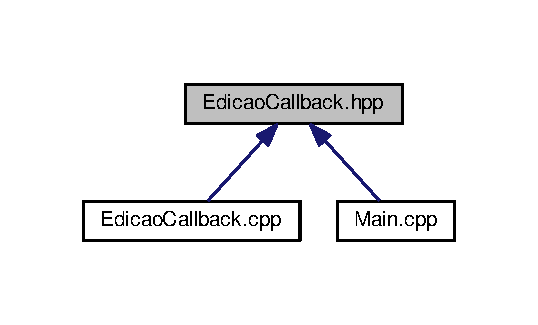
\includegraphics[width=258pt]{EdicaoCallback_8hpp__dep__incl}
\end{center}
\end{figure}
\subsection*{Classes}
\begin{DoxyCompactItemize}
\item 
class \hyperlink{classEdicaoCallback}{Edicao\+Callback}
\begin{DoxyCompactList}\small\item\em Estado da aplicação com relação aos momentos de edição. \end{DoxyCompactList}\end{DoxyCompactItemize}


\subsection{Detailed Description}
Definição do estado de edição. 


\hypertarget{Main_8cpp}{\section{Main.\+cpp File Reference}
\label{Main_8cpp}\index{Main.\+cpp@{Main.\+cpp}}
}
{\ttfamily \#include \char`\"{}Adicao\+Callback.\+hpp\char`\"{}}\\*
{\ttfamily \#include \char`\"{}Edicao\+Callback.\+hpp\char`\"{}}\\*
{\ttfamily \#include \char`\"{}Mundo.\+hpp\char`\"{}}\\*
{\ttfamily \#include $<$ctype.\+h$>$}\\*
Include dependency graph for Main.\+cpp\+:
\nopagebreak
\begin{figure}[H]
\begin{center}
\leavevmode
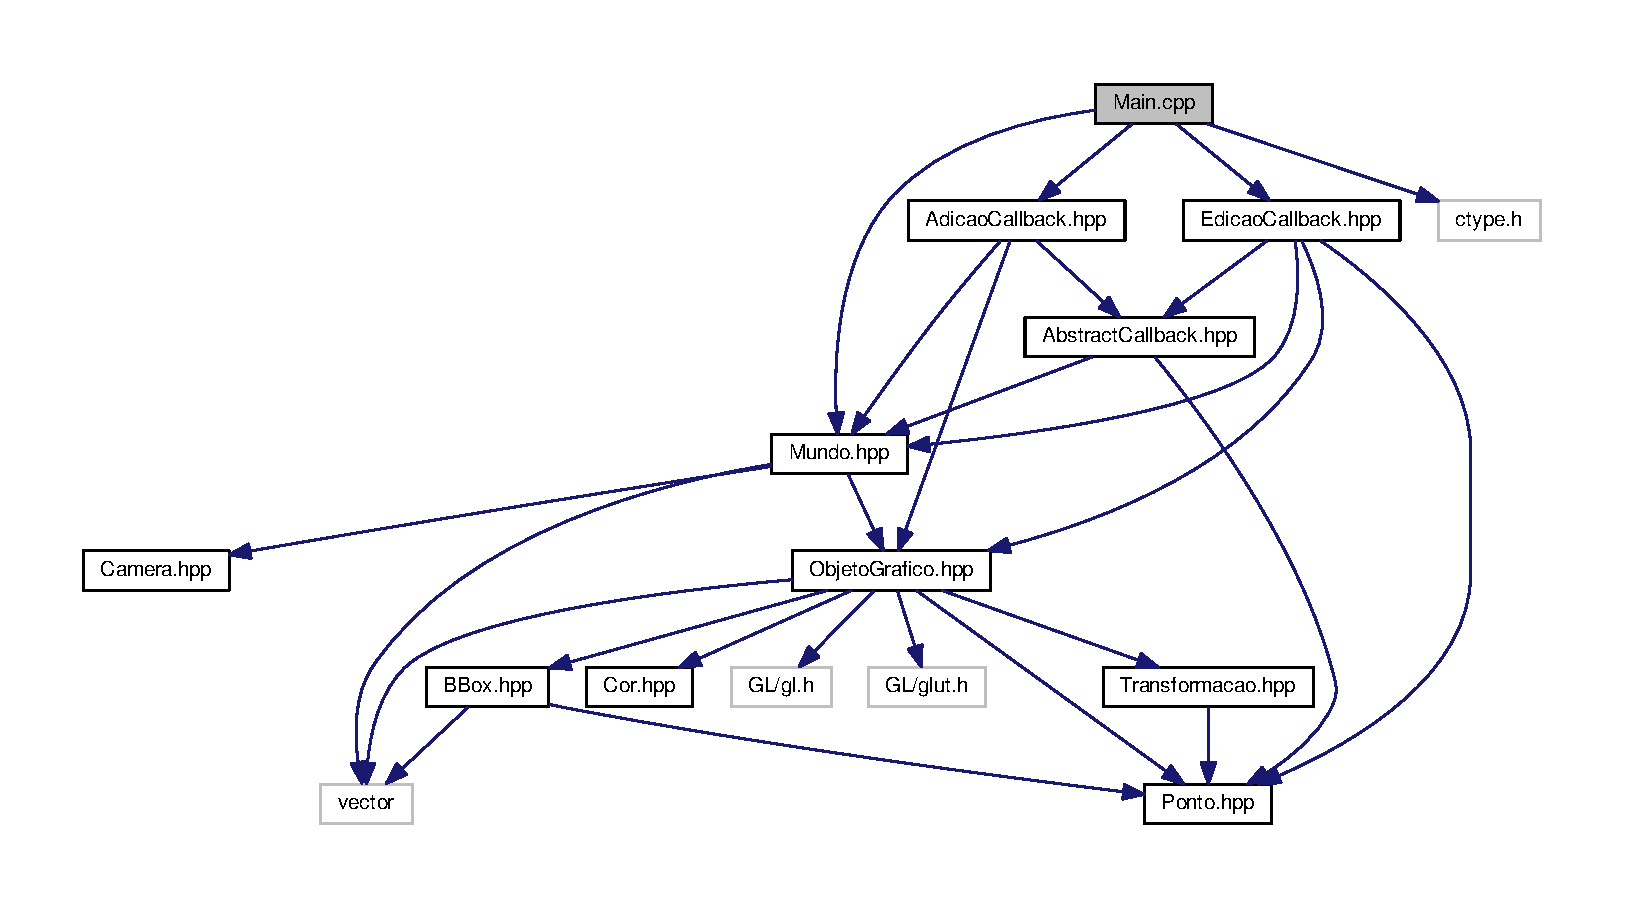
\includegraphics[width=350pt]{Main_8cpp__incl}
\end{center}
\end{figure}
\subsection*{Functions}
\begin{DoxyCompactItemize}
\item 
void \hyperlink{Main_8cpp_a1e5b20fed15743656bb6d2e6a6ea6269}{display} ()
\item 
void \hyperlink{Main_8cpp_aef7ba2f69afb2d954545f64c7fe24b14}{keyboard} (unsigned char key, int x, int y)
\item 
void \hyperlink{Main_8cpp_ac76a5d78172a826cd6ee9512b89a86c0}{mouse} (int button, int state, int x, int y)
\item 
void \hyperlink{Main_8cpp_af995281f4bf85ee669e2ea95930fdf85}{passive\+Motion} (int x, int y)
\item 
void \hyperlink{Main_8cpp_a6819355374dd277347abd7c4235f0cd7}{reshape} (int width, int height)
\item 
void \hyperlink{Main_8cpp_a42b4e1505fa41d975209a6fc5e7f4230}{special} (int key, int x, int y)
\item 
int \hyperlink{Main_8cpp_a0ddf1224851353fc92bfbff6f499fa97}{main} (int argc, char $\ast$argv\mbox{[}$\,$\mbox{]})
\end{DoxyCompactItemize}
\subsection*{Variables}
\begin{DoxyCompactItemize}
\item 
\hyperlink{classMundo}{Mundo} \hyperlink{Main_8cpp_a79514aa758b35d1d1a8c227f4b1ad434}{mundo}
\item 
\hyperlink{classAdicaoCallback}{Adicao\+Callback} \hyperlink{Main_8cpp_aee30e7a7d561101de7dea87827cdc66f}{adicao\+Callback} (\hyperlink{Main_8cpp_a79514aa758b35d1d1a8c227f4b1ad434}{mundo})
\item 
\hyperlink{classEdicaoCallback}{Edicao\+Callback} \hyperlink{Main_8cpp_acf31fc540d1690f044f569c59d868f48}{edicao\+Callback} (\hyperlink{Main_8cpp_a79514aa758b35d1d1a8c227f4b1ad434}{mundo})
\item 
\hyperlink{classAbstractCallback}{Abstract\+Callback} $\ast$ \hyperlink{Main_8cpp_afcbe8fc3420c30692d68361de2d8c258}{callback\+Atual}
\end{DoxyCompactItemize}


\subsection{Function Documentation}
\hypertarget{Main_8cpp_a1e5b20fed15743656bb6d2e6a6ea6269}{\index{Main.\+cpp@{Main.\+cpp}!display@{display}}
\index{display@{display}!Main.\+cpp@{Main.\+cpp}}
\subsubsection[{display}]{\setlength{\rightskip}{0pt plus 5cm}void display (
\begin{DoxyParamCaption}
{}
\end{DoxyParamCaption}
)}}\label{Main_8cpp_a1e5b20fed15743656bb6d2e6a6ea6269}
Function called by G\+L\+U\+T to render the scene. \hypertarget{Main_8cpp_aef7ba2f69afb2d954545f64c7fe24b14}{\index{Main.\+cpp@{Main.\+cpp}!keyboard@{keyboard}}
\index{keyboard@{keyboard}!Main.\+cpp@{Main.\+cpp}}
\subsubsection[{keyboard}]{\setlength{\rightskip}{0pt plus 5cm}void keyboard (
\begin{DoxyParamCaption}
\item[{unsigned char}]{key, }
\item[{int}]{x, }
\item[{int}]{y}
\end{DoxyParamCaption}
)}}\label{Main_8cpp_aef7ba2f69afb2d954545f64c7fe24b14}
Function called by G\+L\+U\+T to handle keypresses \hypertarget{Main_8cpp_a0ddf1224851353fc92bfbff6f499fa97}{\index{Main.\+cpp@{Main.\+cpp}!main@{main}}
\index{main@{main}!Main.\+cpp@{Main.\+cpp}}
\subsubsection[{main}]{\setlength{\rightskip}{0pt plus 5cm}int main (
\begin{DoxyParamCaption}
\item[{int}]{argc, }
\item[{char $\ast$}]{argv\mbox{[}$\,$\mbox{]}}
\end{DoxyParamCaption}
)}}\label{Main_8cpp_a0ddf1224851353fc92bfbff6f499fa97}
\hypertarget{Main_8cpp_ac76a5d78172a826cd6ee9512b89a86c0}{\index{Main.\+cpp@{Main.\+cpp}!mouse@{mouse}}
\index{mouse@{mouse}!Main.\+cpp@{Main.\+cpp}}
\subsubsection[{mouse}]{\setlength{\rightskip}{0pt plus 5cm}void mouse (
\begin{DoxyParamCaption}
\item[{int}]{button, }
\item[{int}]{state, }
\item[{int}]{x, }
\item[{int}]{y}
\end{DoxyParamCaption}
)}}\label{Main_8cpp_ac76a5d78172a826cd6ee9512b89a86c0}
Function called by G\+L\+U\+T when a mouse button is pressed. \hypertarget{Main_8cpp_af995281f4bf85ee669e2ea95930fdf85}{\index{Main.\+cpp@{Main.\+cpp}!passive\+Motion@{passive\+Motion}}
\index{passive\+Motion@{passive\+Motion}!Main.\+cpp@{Main.\+cpp}}
\subsubsection[{passive\+Motion}]{\setlength{\rightskip}{0pt plus 5cm}void passive\+Motion (
\begin{DoxyParamCaption}
\item[{int}]{x, }
\item[{int}]{y}
\end{DoxyParamCaption}
)}}\label{Main_8cpp_af995281f4bf85ee669e2ea95930fdf85}
\hypertarget{Main_8cpp_a6819355374dd277347abd7c4235f0cd7}{\index{Main.\+cpp@{Main.\+cpp}!reshape@{reshape}}
\index{reshape@{reshape}!Main.\+cpp@{Main.\+cpp}}
\subsubsection[{reshape}]{\setlength{\rightskip}{0pt plus 5cm}void reshape (
\begin{DoxyParamCaption}
\item[{int}]{width, }
\item[{int}]{height}
\end{DoxyParamCaption}
)}}\label{Main_8cpp_a6819355374dd277347abd7c4235f0cd7}
\hypertarget{Main_8cpp_a42b4e1505fa41d975209a6fc5e7f4230}{\index{Main.\+cpp@{Main.\+cpp}!special@{special}}
\index{special@{special}!Main.\+cpp@{Main.\+cpp}}
\subsubsection[{special}]{\setlength{\rightskip}{0pt plus 5cm}void special (
\begin{DoxyParamCaption}
\item[{int}]{key, }
\item[{int}]{x, }
\item[{int}]{y}
\end{DoxyParamCaption}
)}}\label{Main_8cpp_a42b4e1505fa41d975209a6fc5e7f4230}


\subsection{Variable Documentation}
\hypertarget{Main_8cpp_aee30e7a7d561101de7dea87827cdc66f}{\index{Main.\+cpp@{Main.\+cpp}!adicao\+Callback@{adicao\+Callback}}
\index{adicao\+Callback@{adicao\+Callback}!Main.\+cpp@{Main.\+cpp}}
\subsubsection[{adicao\+Callback}]{\setlength{\rightskip}{0pt plus 5cm}{\bf Adicao\+Callback} adicao\+Callback({\bf mundo})}}\label{Main_8cpp_aee30e7a7d561101de7dea87827cdc66f}
\hypertarget{Main_8cpp_afcbe8fc3420c30692d68361de2d8c258}{\index{Main.\+cpp@{Main.\+cpp}!callback\+Atual@{callback\+Atual}}
\index{callback\+Atual@{callback\+Atual}!Main.\+cpp@{Main.\+cpp}}
\subsubsection[{callback\+Atual}]{\setlength{\rightskip}{0pt plus 5cm}{\bf Abstract\+Callback}$\ast$ callback\+Atual}}\label{Main_8cpp_afcbe8fc3420c30692d68361de2d8c258}
\hypertarget{Main_8cpp_acf31fc540d1690f044f569c59d868f48}{\index{Main.\+cpp@{Main.\+cpp}!edicao\+Callback@{edicao\+Callback}}
\index{edicao\+Callback@{edicao\+Callback}!Main.\+cpp@{Main.\+cpp}}
\subsubsection[{edicao\+Callback}]{\setlength{\rightskip}{0pt plus 5cm}{\bf Edicao\+Callback} edicao\+Callback({\bf mundo})}}\label{Main_8cpp_acf31fc540d1690f044f569c59d868f48}
\hypertarget{Main_8cpp_a79514aa758b35d1d1a8c227f4b1ad434}{\index{Main.\+cpp@{Main.\+cpp}!mundo@{mundo}}
\index{mundo@{mundo}!Main.\+cpp@{Main.\+cpp}}
\subsubsection[{mundo}]{\setlength{\rightskip}{0pt plus 5cm}{\bf Mundo} mundo}}\label{Main_8cpp_a79514aa758b35d1d1a8c227f4b1ad434}

\hypertarget{Mundo_8cpp}{\section{Mundo.\+cpp File Reference}
\label{Mundo_8cpp}\index{Mundo.\+cpp@{Mundo.\+cpp}}
}
{\ttfamily \#include \char`\"{}Mundo.\+hpp\char`\"{}}\\*
{\ttfamily \#include \char`\"{}Utils.\+hpp\char`\"{}}\\*
{\ttfamily \#include $<$vector$>$}\\*
{\ttfamily \#include $<$G\+L/gl.\+h$>$}\\*
{\ttfamily \#include $<$G\+L/glut.\+h$>$}\\*
{\ttfamily \#include $<$algorithm$>$}\\*
Include dependency graph for Mundo.\+cpp\+:
\nopagebreak
\begin{figure}[H]
\begin{center}
\leavevmode
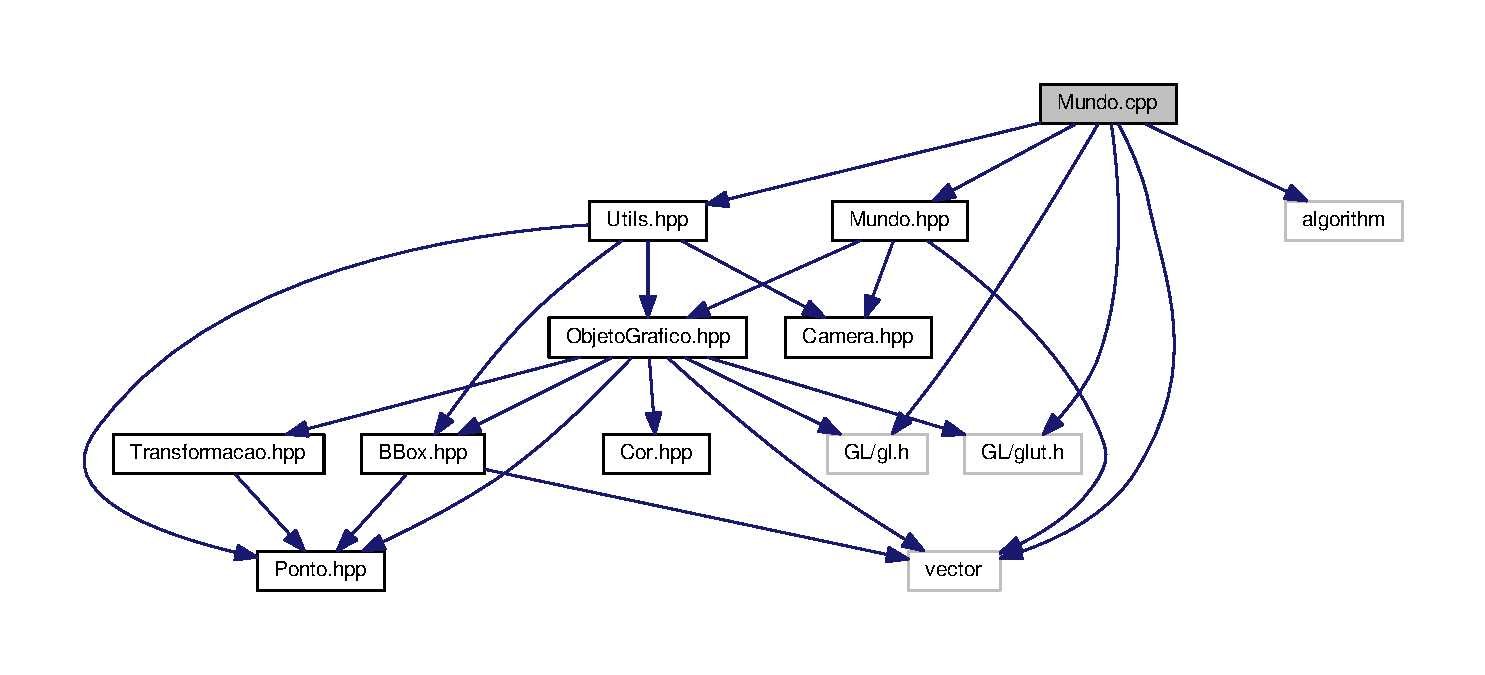
\includegraphics[width=350pt]{Mundo_8cpp__incl}
\end{center}
\end{figure}

\hypertarget{Mundo_8hpp}{\section{Mundo.\+hpp File Reference}
\label{Mundo_8hpp}\index{Mundo.\+hpp@{Mundo.\+hpp}}
}


Definição de \hyperlink{classMundo}{Mundo} par o Trabalho N3 de C\+G.  


{\ttfamily \#include \char`\"{}Objeto\+Grafico.\+hpp\char`\"{}}\\*
{\ttfamily \#include \char`\"{}Camera.\+hpp\char`\"{}}\\*
{\ttfamily \#include $<$vector$>$}\\*
Include dependency graph for Mundo.\+hpp\+:
\nopagebreak
\begin{figure}[H]
\begin{center}
\leavevmode
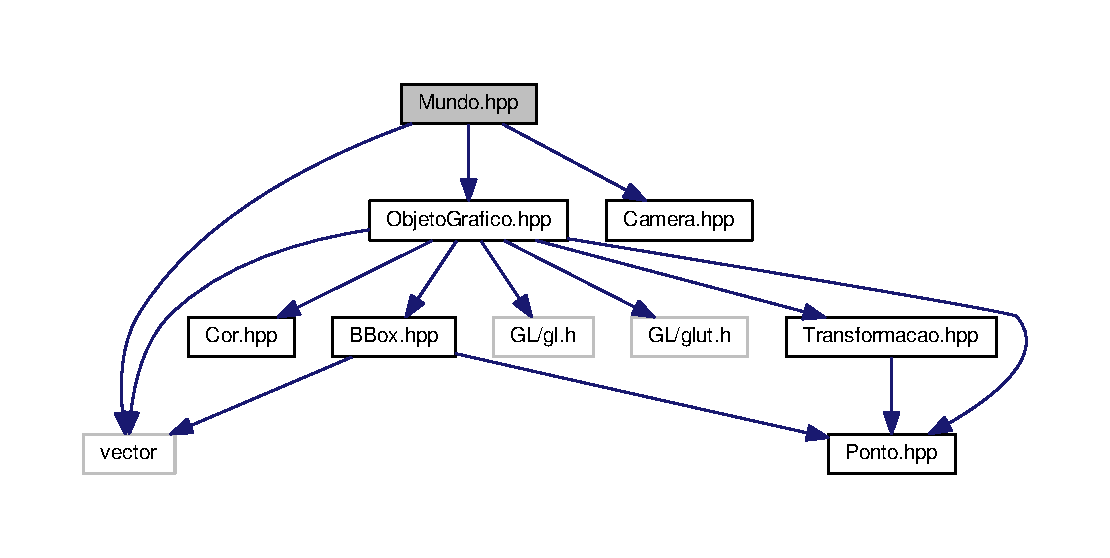
\includegraphics[width=350pt]{Mundo_8hpp__incl}
\end{center}
\end{figure}
This graph shows which files directly or indirectly include this file\+:
\nopagebreak
\begin{figure}[H]
\begin{center}
\leavevmode
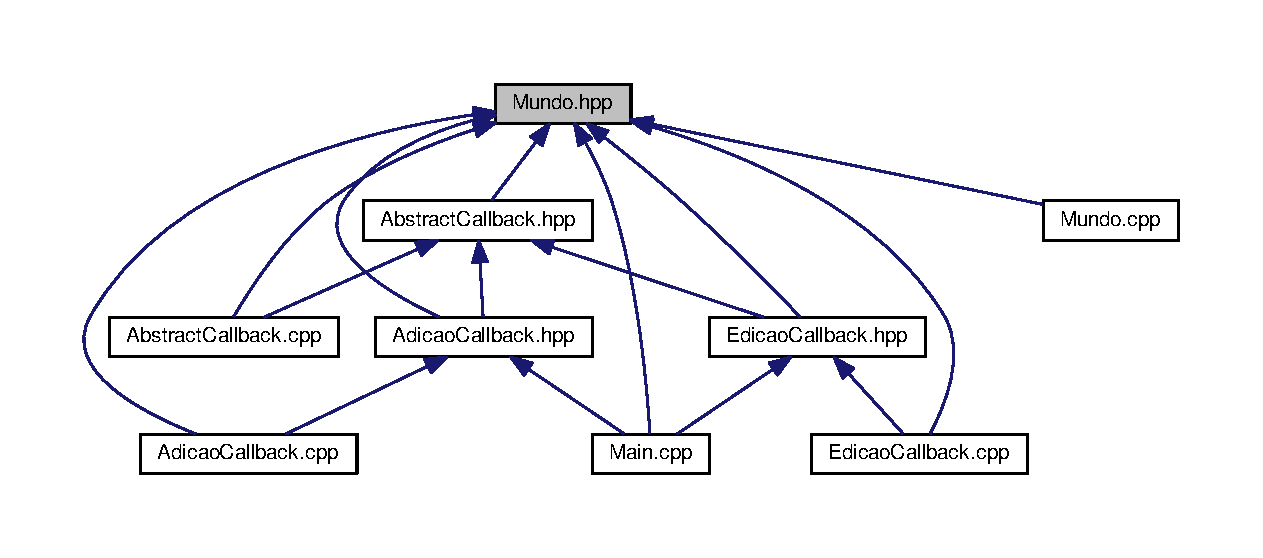
\includegraphics[width=350pt]{Mundo_8hpp__dep__incl}
\end{center}
\end{figure}
\subsection*{Classes}
\begin{DoxyCompactItemize}
\item 
class \hyperlink{classMundo}{Mundo}
\begin{DoxyCompactList}\small\item\em O Universo gráfico. \end{DoxyCompactList}\end{DoxyCompactItemize}


\subsection{Detailed Description}
Definição de \hyperlink{classMundo}{Mundo} par o Trabalho N3 de C\+G. 


\hypertarget{ObjetoGrafico_8cpp}{\section{Objeto\+Grafico.\+cpp File Reference}
\label{ObjetoGrafico_8cpp}\index{Objeto\+Grafico.\+cpp@{Objeto\+Grafico.\+cpp}}
}
{\ttfamily \#include \char`\"{}Objeto\+Grafico.\+hpp\char`\"{}}\\*
{\ttfamily \#include \char`\"{}Utils.\+hpp\char`\"{}}\\*
{\ttfamily \#include $<$G\+L/gl.\+h$>$}\\*
{\ttfamily \#include $<$G\+L/glut.\+h$>$}\\*
{\ttfamily \#include $<$algorithm$>$}\\*
Include dependency graph for Objeto\+Grafico.\+cpp\+:
\nopagebreak
\begin{figure}[H]
\begin{center}
\leavevmode
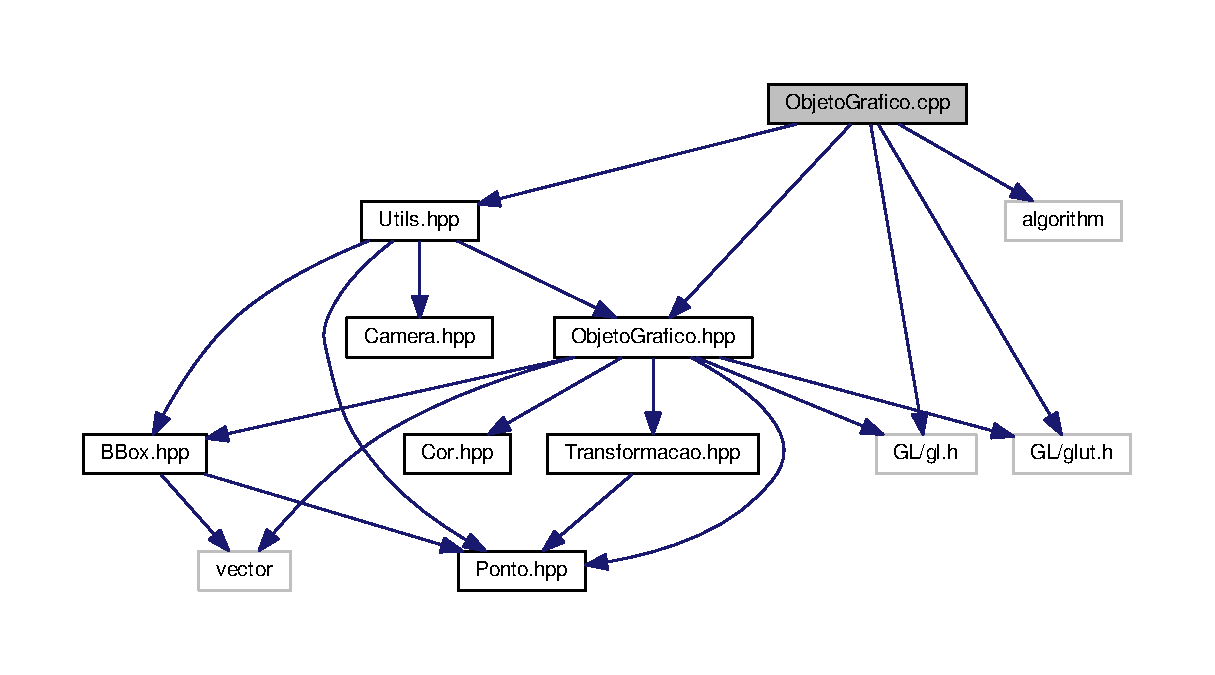
\includegraphics[width=350pt]{ObjetoGrafico_8cpp__incl}
\end{center}
\end{figure}
\subsection*{Variables}
\begin{DoxyCompactItemize}
\item 
const double \hyperlink{ObjetoGrafico_8cpp_a536cf34e9e5f76c63ba8960f2a849773}{S\+E\+L\+E\+C\+T\+I\+O\+N\+\_\+\+D\+I\+S\+T\+A\+N\+C\+E} = 5 $\ast$ 5
\end{DoxyCompactItemize}


\subsection{Variable Documentation}
\hypertarget{ObjetoGrafico_8cpp_a536cf34e9e5f76c63ba8960f2a849773}{\index{Objeto\+Grafico.\+cpp@{Objeto\+Grafico.\+cpp}!S\+E\+L\+E\+C\+T\+I\+O\+N\+\_\+\+D\+I\+S\+T\+A\+N\+C\+E@{S\+E\+L\+E\+C\+T\+I\+O\+N\+\_\+\+D\+I\+S\+T\+A\+N\+C\+E}}
\index{S\+E\+L\+E\+C\+T\+I\+O\+N\+\_\+\+D\+I\+S\+T\+A\+N\+C\+E@{S\+E\+L\+E\+C\+T\+I\+O\+N\+\_\+\+D\+I\+S\+T\+A\+N\+C\+E}!Objeto\+Grafico.\+cpp@{Objeto\+Grafico.\+cpp}}
\subsubsection[{S\+E\+L\+E\+C\+T\+I\+O\+N\+\_\+\+D\+I\+S\+T\+A\+N\+C\+E}]{\setlength{\rightskip}{0pt plus 5cm}const double S\+E\+L\+E\+C\+T\+I\+O\+N\+\_\+\+D\+I\+S\+T\+A\+N\+C\+E = 5 $\ast$ 5}}\label{ObjetoGrafico_8cpp_a536cf34e9e5f76c63ba8960f2a849773}

\hypertarget{ObjetoGrafico_8hpp}{\section{Objeto\+Grafico.\+hpp File Reference}
\label{ObjetoGrafico_8hpp}\index{Objeto\+Grafico.\+hpp@{Objeto\+Grafico.\+hpp}}
}


Definição de Ojeto Gráfico.  


{\ttfamily \#include \char`\"{}B\+Box.\+hpp\char`\"{}}\\*
{\ttfamily \#include \char`\"{}Cor.\+hpp\char`\"{}}\\*
{\ttfamily \#include \char`\"{}Ponto.\+hpp\char`\"{}}\\*
{\ttfamily \#include \char`\"{}Transformacao.\+hpp\char`\"{}}\\*
{\ttfamily \#include $<$vector$>$}\\*
{\ttfamily \#include $<$G\+L/gl.\+h$>$}\\*
{\ttfamily \#include $<$G\+L/glut.\+h$>$}\\*
Include dependency graph for Objeto\+Grafico.\+hpp\+:
\nopagebreak
\begin{figure}[H]
\begin{center}
\leavevmode
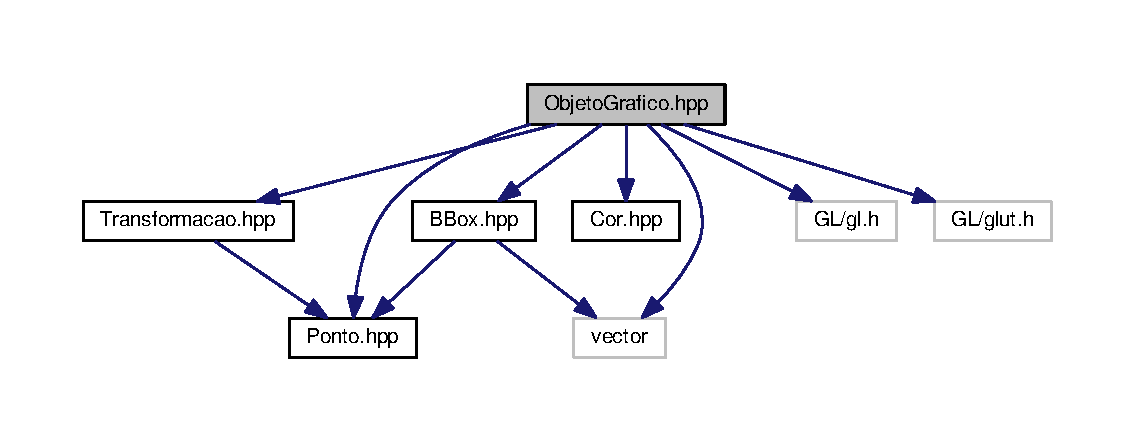
\includegraphics[width=350pt]{ObjetoGrafico_8hpp__incl}
\end{center}
\end{figure}
This graph shows which files directly or indirectly include this file\+:
\nopagebreak
\begin{figure}[H]
\begin{center}
\leavevmode
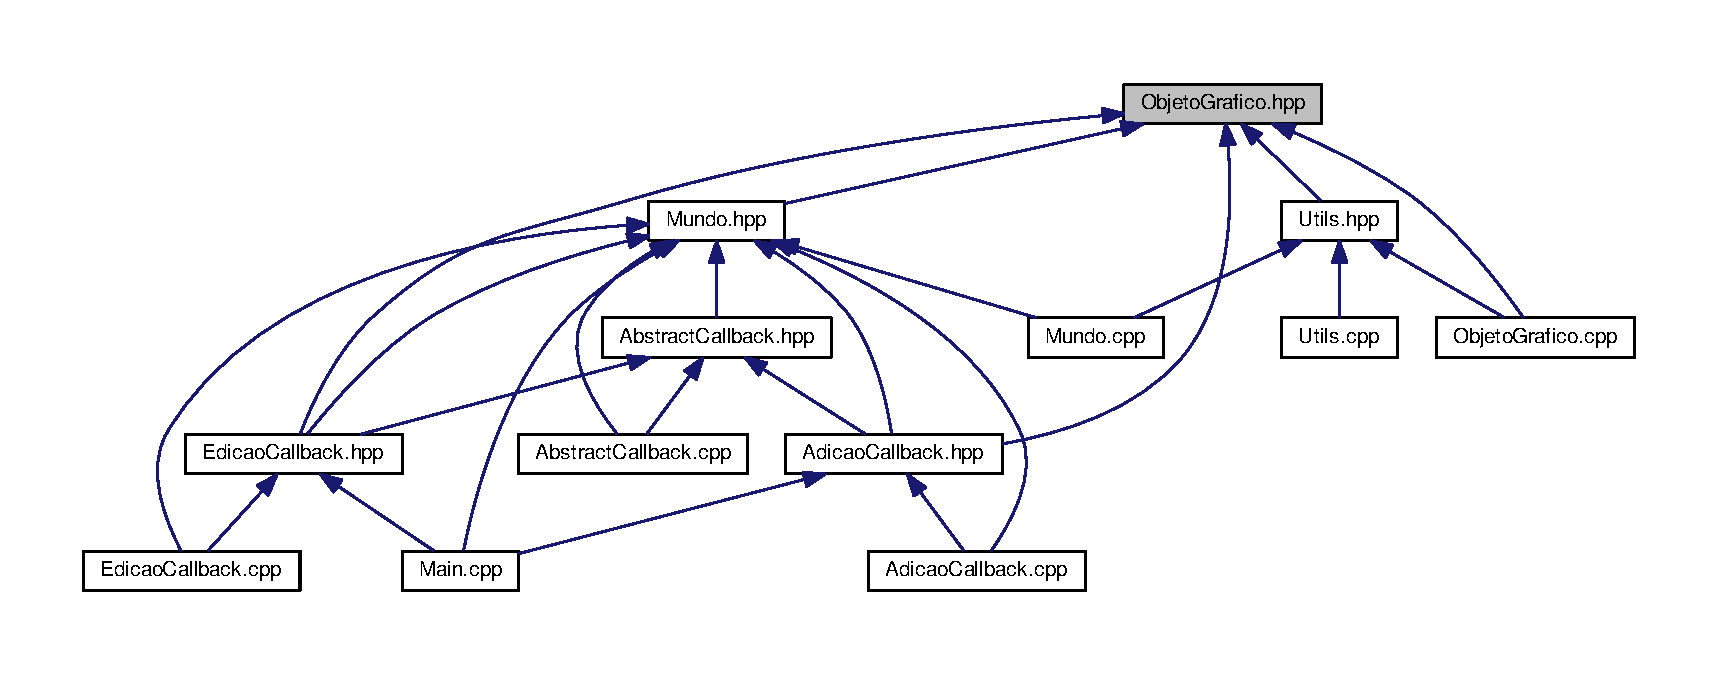
\includegraphics[width=350pt]{ObjetoGrafico_8hpp__dep__incl}
\end{center}
\end{figure}
\subsection*{Classes}
\begin{DoxyCompactItemize}
\item 
class \hyperlink{classObjetoGrafico}{Objeto\+Grafico}
\begin{DoxyCompactList}\small\item\em Um Objeto Grafico do mundo. \end{DoxyCompactList}\end{DoxyCompactItemize}


\subsection{Detailed Description}
Definição de Ojeto Gráfico. 


\hypertarget{Ponto_8cpp}{\section{Ponto.\+cpp File Reference}
\label{Ponto_8cpp}\index{Ponto.\+cpp@{Ponto.\+cpp}}
}
{\ttfamily \#include \char`\"{}Ponto.\+hpp\char`\"{}}\\*
Include dependency graph for Ponto.\+cpp\+:
\nopagebreak
\begin{figure}[H]
\begin{center}
\leavevmode
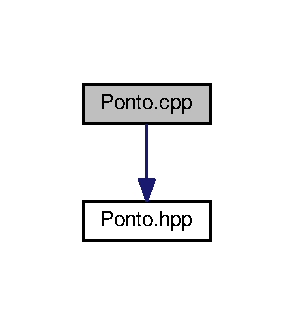
\includegraphics[width=141pt]{Ponto_8cpp__incl}
\end{center}
\end{figure}
\subsection*{Functions}
\begin{DoxyCompactItemize}
\item 
bool \hyperlink{Ponto_8cpp_a785b5b643cf32d3bde762e4c5ce4369e}{operator==} (const \hyperlink{classPonto}{Ponto} \&este, const \hyperlink{classPonto}{Ponto} \&outro)
\item 
\hyperlink{classPonto}{Ponto} \hyperlink{Ponto_8cpp_a66166b646f2346ec712f3894c7d6f387}{operator-\/} (const \hyperlink{classPonto}{Ponto} \&ponto)
\end{DoxyCompactItemize}


\subsection{Function Documentation}
\hypertarget{Ponto_8cpp_a66166b646f2346ec712f3894c7d6f387}{\index{Ponto.\+cpp@{Ponto.\+cpp}!operator-\/@{operator-\/}}
\index{operator-\/@{operator-\/}!Ponto.\+cpp@{Ponto.\+cpp}}
\subsubsection[{operator-\/}]{\setlength{\rightskip}{0pt plus 5cm}{\bf Ponto} operator-\/ (
\begin{DoxyParamCaption}
\item[{const {\bf Ponto} \&}]{ponto}
\end{DoxyParamCaption}
)}}\label{Ponto_8cpp_a66166b646f2346ec712f3894c7d6f387}
Inverte um ponto. \hypertarget{Ponto_8cpp_a785b5b643cf32d3bde762e4c5ce4369e}{\index{Ponto.\+cpp@{Ponto.\+cpp}!operator==@{operator==}}
\index{operator==@{operator==}!Ponto.\+cpp@{Ponto.\+cpp}}
\subsubsection[{operator==}]{\setlength{\rightskip}{0pt plus 5cm}bool operator== (
\begin{DoxyParamCaption}
\item[{const {\bf Ponto} \&}]{este, }
\item[{const {\bf Ponto} \&}]{outro}
\end{DoxyParamCaption}
)}}\label{Ponto_8cpp_a785b5b643cf32d3bde762e4c5ce4369e}
Compara se dois pontos são iguais 
\hypertarget{Ponto_8hpp}{\section{Ponto.\+hpp File Reference}
\label{Ponto_8hpp}\index{Ponto.\+hpp@{Ponto.\+hpp}}
}


Definicao de \hyperlink{classPonto}{Ponto}.  


This graph shows which files directly or indirectly include this file\+:
\nopagebreak
\begin{figure}[H]
\begin{center}
\leavevmode
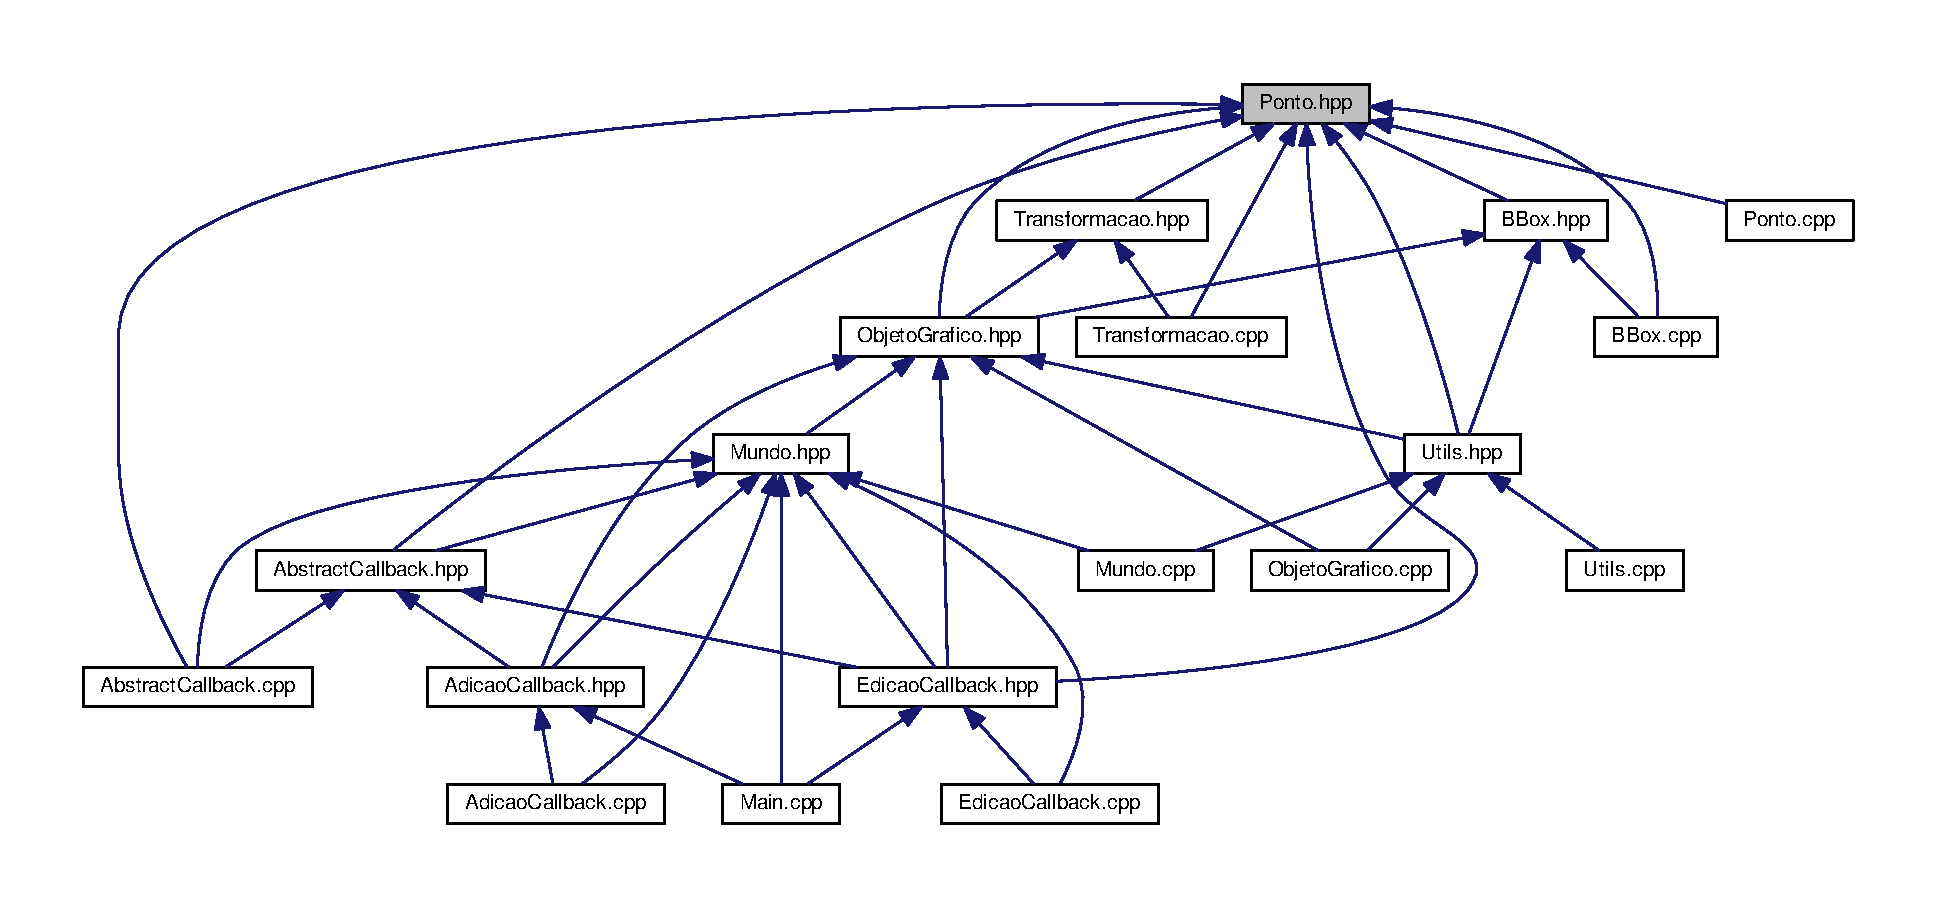
\includegraphics[width=350pt]{Ponto_8hpp__dep__incl}
\end{center}
\end{figure}
\subsection*{Classes}
\begin{DoxyCompactItemize}
\item 
class \hyperlink{classPonto}{Ponto}
\begin{DoxyCompactList}\small\item\em \hyperlink{classPonto}{Ponto} 3\+D. \end{DoxyCompactList}\end{DoxyCompactItemize}
\subsection*{Functions}
\begin{DoxyCompactItemize}
\item 
bool \hyperlink{Ponto_8hpp_a785b5b643cf32d3bde762e4c5ce4369e}{operator==} (const \hyperlink{classPonto}{Ponto} \&este, const \hyperlink{classPonto}{Ponto} \&outro)
\item 
\hyperlink{classPonto}{Ponto} \hyperlink{Ponto_8hpp_a66166b646f2346ec712f3894c7d6f387}{operator-\/} (const \hyperlink{classPonto}{Ponto} \&ponto)
\end{DoxyCompactItemize}


\subsection{Detailed Description}
Definicao de \hyperlink{classPonto}{Ponto}. 



\subsection{Function Documentation}
\hypertarget{Ponto_8hpp_a66166b646f2346ec712f3894c7d6f387}{\index{Ponto.\+hpp@{Ponto.\+hpp}!operator-\/@{operator-\/}}
\index{operator-\/@{operator-\/}!Ponto.\+hpp@{Ponto.\+hpp}}
\subsubsection[{operator-\/}]{\setlength{\rightskip}{0pt plus 5cm}{\bf Ponto} operator-\/ (
\begin{DoxyParamCaption}
\item[{const {\bf Ponto} \&}]{ponto}
\end{DoxyParamCaption}
)}}\label{Ponto_8hpp_a66166b646f2346ec712f3894c7d6f387}
Inverte um ponto. \hypertarget{Ponto_8hpp_a785b5b643cf32d3bde762e4c5ce4369e}{\index{Ponto.\+hpp@{Ponto.\+hpp}!operator==@{operator==}}
\index{operator==@{operator==}!Ponto.\+hpp@{Ponto.\+hpp}}
\subsubsection[{operator==}]{\setlength{\rightskip}{0pt plus 5cm}bool operator== (
\begin{DoxyParamCaption}
\item[{const {\bf Ponto} \&}]{este, }
\item[{const {\bf Ponto} \&}]{outro}
\end{DoxyParamCaption}
)}}\label{Ponto_8hpp_a785b5b643cf32d3bde762e4c5ce4369e}
Compara se dois pontos são iguais 
\hypertarget{Transformacao_8cpp}{\section{Transformacao.\+cpp File Reference}
\label{Transformacao_8cpp}\index{Transformacao.\+cpp@{Transformacao.\+cpp}}
}
{\ttfamily \#include \char`\"{}Transformacao.\+hpp\char`\"{}}\\*
{\ttfamily \#include \char`\"{}Ponto.\+hpp\char`\"{}}\\*
{\ttfamily \#include $<$cmath$>$}\\*
Include dependency graph for Transformacao.\+cpp\+:
\nopagebreak
\begin{figure}[H]
\begin{center}
\leavevmode
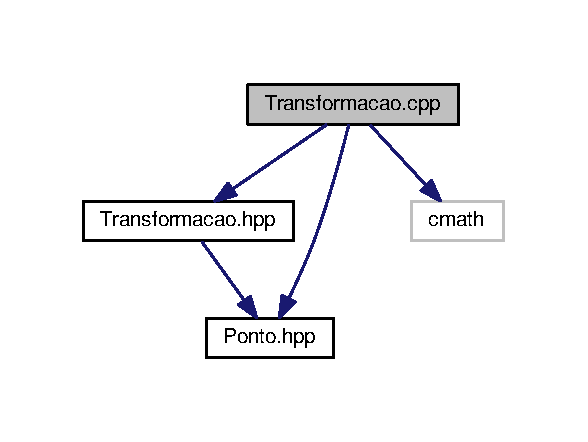
\includegraphics[width=282pt]{Transformacao_8cpp__incl}
\end{center}
\end{figure}

\hypertarget{Transformacao_8hpp}{\section{Transformacao.\+hpp File Reference}
\label{Transformacao_8hpp}\index{Transformacao.\+hpp@{Transformacao.\+hpp}}
}


Definição de \hyperlink{classTransformacao}{Transformacao}.  


{\ttfamily \#include \char`\"{}Ponto.\+hpp\char`\"{}}\\*
Include dependency graph for Transformacao.\+hpp\+:
\nopagebreak
\begin{figure}[H]
\begin{center}
\leavevmode
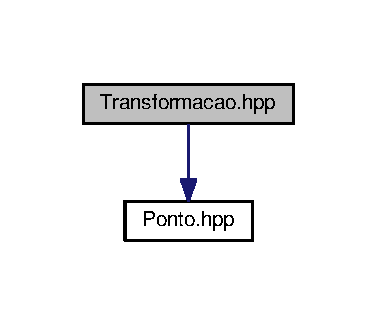
\includegraphics[width=181pt]{Transformacao_8hpp__incl}
\end{center}
\end{figure}
This graph shows which files directly or indirectly include this file\+:
\nopagebreak
\begin{figure}[H]
\begin{center}
\leavevmode
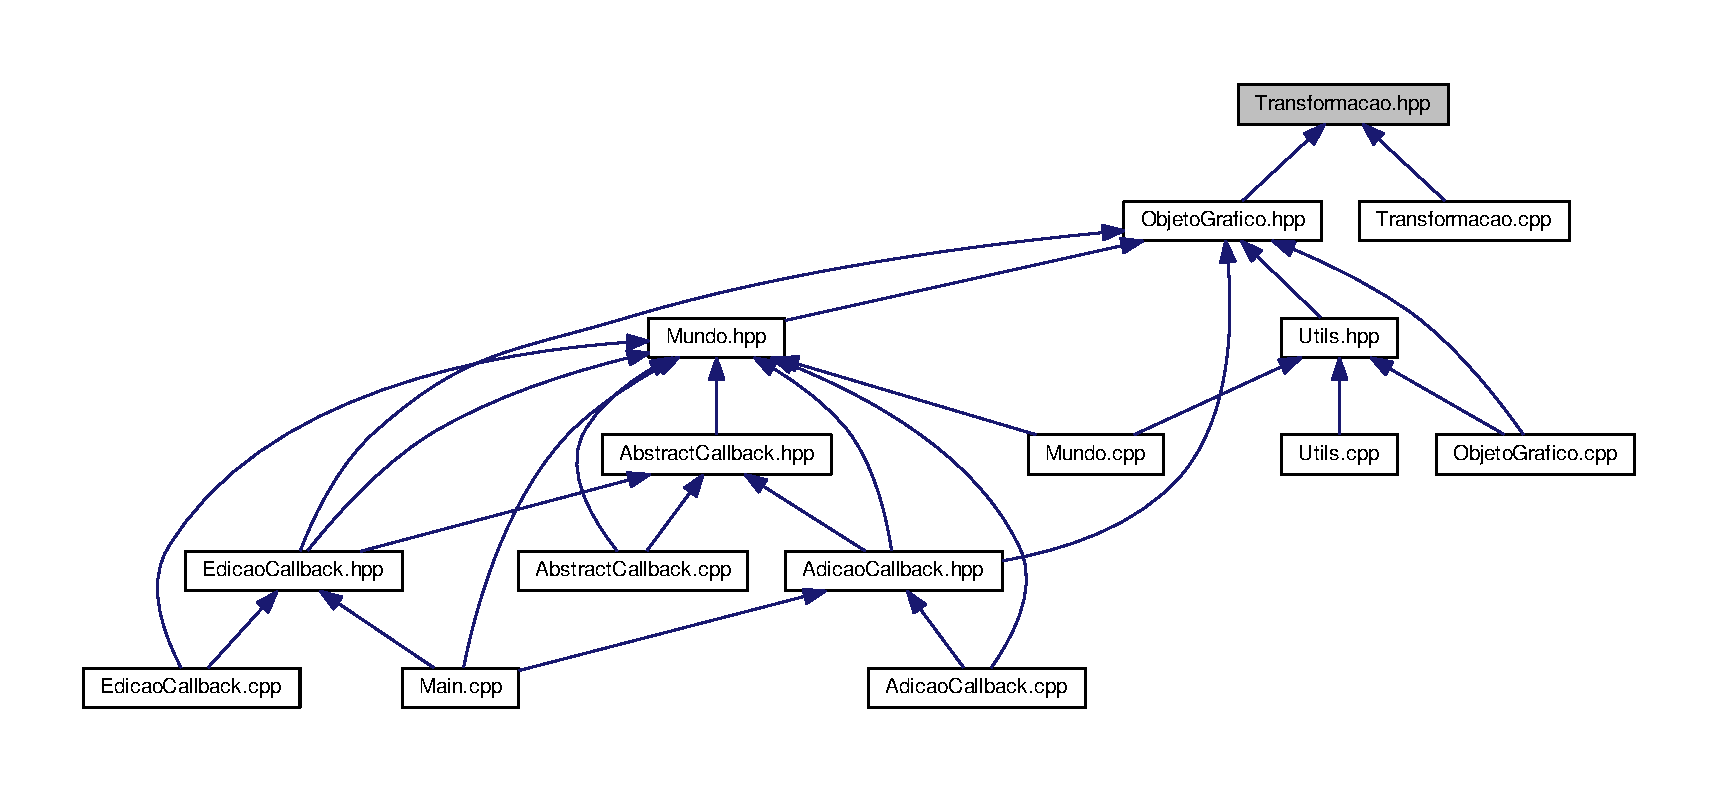
\includegraphics[width=350pt]{Transformacao_8hpp__dep__incl}
\end{center}
\end{figure}
\subsection*{Classes}
\begin{DoxyCompactItemize}
\item 
class \hyperlink{classTransformacao}{Transformacao}
\begin{DoxyCompactList}\small\item\em Uma transformação linear. \end{DoxyCompactList}\end{DoxyCompactItemize}


\subsection{Detailed Description}
Definição de \hyperlink{classTransformacao}{Transformacao}. 


\hypertarget{Utils_8cpp}{\section{Utils.\+cpp File Reference}
\label{Utils_8cpp}\index{Utils.\+cpp@{Utils.\+cpp}}
}
{\ttfamily \#include \char`\"{}Utils.\+hpp\char`\"{}}\\*
Include dependency graph for Utils.\+cpp\+:
\nopagebreak
\begin{figure}[H]
\begin{center}
\leavevmode
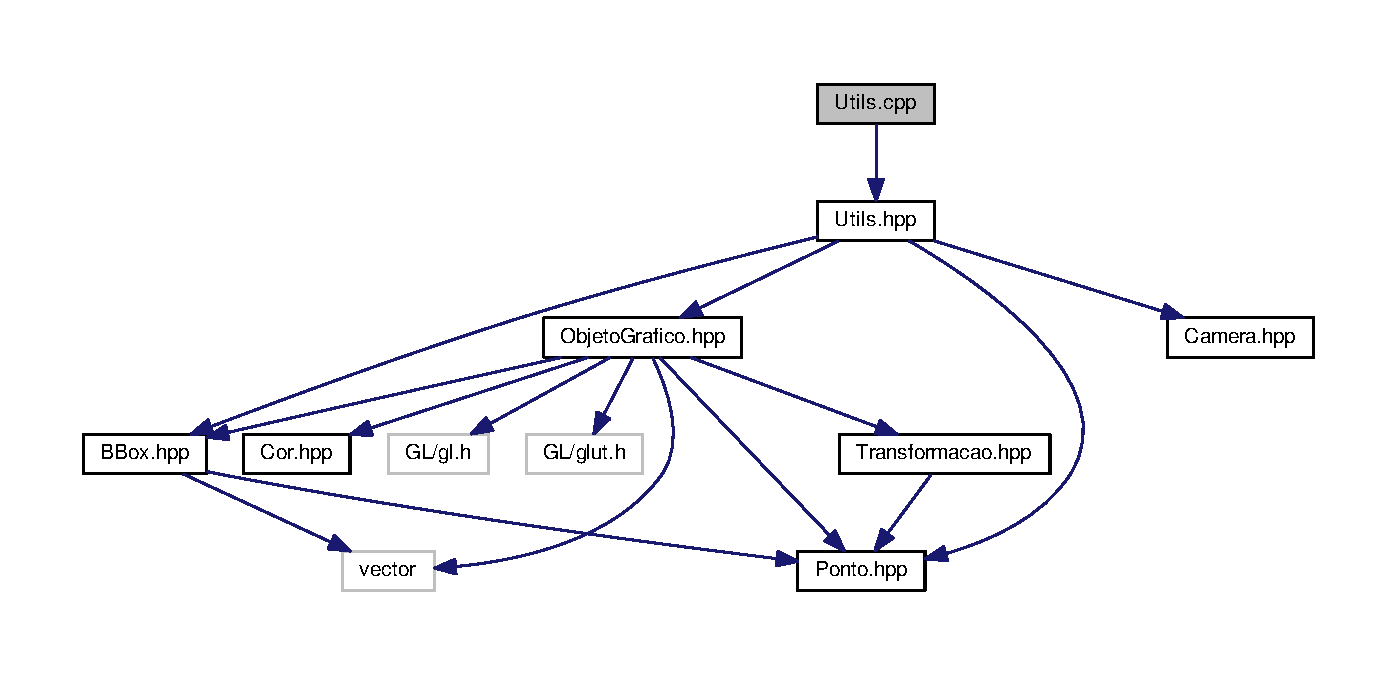
\includegraphics[width=350pt]{Utils_8cpp__incl}
\end{center}
\end{figure}
\subsection*{Functions}
\begin{DoxyCompactItemize}
\item 
\hyperlink{classObjetoGrafico}{Objeto\+Grafico} \hyperlink{Utils_8cpp_ad1fcbfb8492a5f9c82183017bd9113aa}{bbox\+To\+Objeto} (const \hyperlink{classBBox}{B\+Box} \&bbox)
\item 
\hyperlink{classObjetoGrafico}{Objeto\+Grafico} \hyperlink{Utils_8cpp_a90e1c847d715881c8d76d2be252d037f}{eixos\+Referencia\+As\+Objeto\+Grafico} ()
\item 
\hyperlink{classCamera}{Camera} \hyperlink{Utils_8cpp_a24732334b6ada8720b0ac13445155552}{obtem\+Camera} ()
\item 
double \hyperlink{Utils_8cpp_a3b318b63385acf7b8cde73a3800fc112}{dist} (const \hyperlink{classPonto}{Ponto} \&lhs, const \hyperlink{classPonto}{Ponto} \&rhs)
\end{DoxyCompactItemize}


\subsection{Function Documentation}
\hypertarget{Utils_8cpp_ad1fcbfb8492a5f9c82183017bd9113aa}{\index{Utils.\+cpp@{Utils.\+cpp}!bbox\+To\+Objeto@{bbox\+To\+Objeto}}
\index{bbox\+To\+Objeto@{bbox\+To\+Objeto}!Utils.\+cpp@{Utils.\+cpp}}
\subsubsection[{bbox\+To\+Objeto}]{\setlength{\rightskip}{0pt plus 5cm}{\bf Objeto\+Grafico} bbox\+To\+Objeto (
\begin{DoxyParamCaption}
\item[{const {\bf B\+Box} \&}]{bbox}
\end{DoxyParamCaption}
)}}\label{Utils_8cpp_ad1fcbfb8492a5f9c82183017bd9113aa}
Cria uma representação grafica da \hyperlink{classBBox}{B\+Box} \hypertarget{Utils_8cpp_a3b318b63385acf7b8cde73a3800fc112}{\index{Utils.\+cpp@{Utils.\+cpp}!dist@{dist}}
\index{dist@{dist}!Utils.\+cpp@{Utils.\+cpp}}
\subsubsection[{dist}]{\setlength{\rightskip}{0pt plus 5cm}double dist (
\begin{DoxyParamCaption}
\item[{const {\bf Ponto} \&}]{lhs, }
\item[{const {\bf Ponto} \&}]{rhs}
\end{DoxyParamCaption}
)}}\label{Utils_8cpp_a3b318b63385acf7b8cde73a3800fc112}
Calcula a distancia {\bfseries ao quadrado} entre dois pontos. \hypertarget{Utils_8cpp_a90e1c847d715881c8d76d2be252d037f}{\index{Utils.\+cpp@{Utils.\+cpp}!eixos\+Referencia\+As\+Objeto\+Grafico@{eixos\+Referencia\+As\+Objeto\+Grafico}}
\index{eixos\+Referencia\+As\+Objeto\+Grafico@{eixos\+Referencia\+As\+Objeto\+Grafico}!Utils.\+cpp@{Utils.\+cpp}}
\subsubsection[{eixos\+Referencia\+As\+Objeto\+Grafico}]{\setlength{\rightskip}{0pt plus 5cm}{\bf Objeto\+Grafico} eixos\+Referencia\+As\+Objeto\+Grafico (
\begin{DoxyParamCaption}
{}
\end{DoxyParamCaption}
)}}\label{Utils_8cpp_a90e1c847d715881c8d76d2be252d037f}
Cria um objeto grafico com os eixos \hypertarget{Utils_8cpp_a24732334b6ada8720b0ac13445155552}{\index{Utils.\+cpp@{Utils.\+cpp}!obtem\+Camera@{obtem\+Camera}}
\index{obtem\+Camera@{obtem\+Camera}!Utils.\+cpp@{Utils.\+cpp}}
\subsubsection[{obtem\+Camera}]{\setlength{\rightskip}{0pt plus 5cm}{\bf Camera} obtem\+Camera (
\begin{DoxyParamCaption}
{}
\end{DoxyParamCaption}
)}}\label{Utils_8cpp_a24732334b6ada8720b0ac13445155552}
Obtem uma instancia da camera para o mundo 
\hypertarget{Utils_8hpp}{\section{Utils.\+hpp File Reference}
\label{Utils_8hpp}\index{Utils.\+hpp@{Utils.\+hpp}}
}
{\ttfamily \#include \char`\"{}B\+Box.\+hpp\char`\"{}}\\*
{\ttfamily \#include \char`\"{}Objeto\+Grafico.\+hpp\char`\"{}}\\*
{\ttfamily \#include \char`\"{}Ponto.\+hpp\char`\"{}}\\*
{\ttfamily \#include \char`\"{}Camera.\+hpp\char`\"{}}\\*
Include dependency graph for Utils.\+hpp\+:
\nopagebreak
\begin{figure}[H]
\begin{center}
\leavevmode
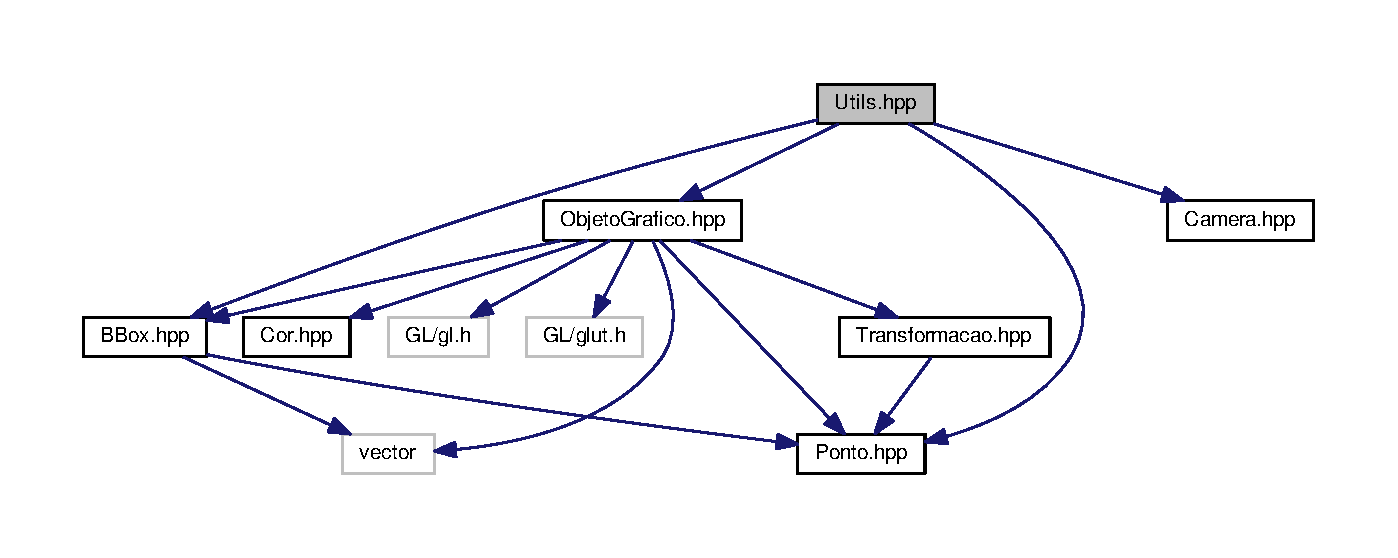
\includegraphics[width=350pt]{Utils_8hpp__incl}
\end{center}
\end{figure}
This graph shows which files directly or indirectly include this file\+:
\nopagebreak
\begin{figure}[H]
\begin{center}
\leavevmode
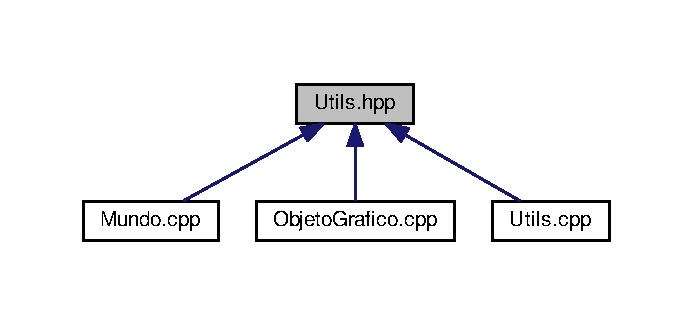
\includegraphics[width=333pt]{Utils_8hpp__dep__incl}
\end{center}
\end{figure}
\subsection*{Functions}
\begin{DoxyCompactItemize}
\item 
\hyperlink{classObjetoGrafico}{Objeto\+Grafico} \hyperlink{Utils_8hpp_ad1fcbfb8492a5f9c82183017bd9113aa}{bbox\+To\+Objeto} (const \hyperlink{classBBox}{B\+Box} \&bbox)
\item 
\hyperlink{classObjetoGrafico}{Objeto\+Grafico} \hyperlink{Utils_8hpp_a90e1c847d715881c8d76d2be252d037f}{eixos\+Referencia\+As\+Objeto\+Grafico} ()
\item 
double \hyperlink{Utils_8hpp_a3b318b63385acf7b8cde73a3800fc112}{dist} (const \hyperlink{classPonto}{Ponto} \&lhs, const \hyperlink{classPonto}{Ponto} \&rhs)
\item 
\hyperlink{classCamera}{Camera} \hyperlink{Utils_8hpp_a24732334b6ada8720b0ac13445155552}{obtem\+Camera} ()
\end{DoxyCompactItemize}


\subsection{Function Documentation}
\hypertarget{Utils_8hpp_ad1fcbfb8492a5f9c82183017bd9113aa}{\index{Utils.\+hpp@{Utils.\+hpp}!bbox\+To\+Objeto@{bbox\+To\+Objeto}}
\index{bbox\+To\+Objeto@{bbox\+To\+Objeto}!Utils.\+hpp@{Utils.\+hpp}}
\subsubsection[{bbox\+To\+Objeto}]{\setlength{\rightskip}{0pt plus 5cm}{\bf Objeto\+Grafico} bbox\+To\+Objeto (
\begin{DoxyParamCaption}
\item[{const {\bf B\+Box} \&}]{bbox}
\end{DoxyParamCaption}
)}}\label{Utils_8hpp_ad1fcbfb8492a5f9c82183017bd9113aa}
Cria uma representação grafica da \hyperlink{classBBox}{B\+Box} \hypertarget{Utils_8hpp_a3b318b63385acf7b8cde73a3800fc112}{\index{Utils.\+hpp@{Utils.\+hpp}!dist@{dist}}
\index{dist@{dist}!Utils.\+hpp@{Utils.\+hpp}}
\subsubsection[{dist}]{\setlength{\rightskip}{0pt plus 5cm}double dist (
\begin{DoxyParamCaption}
\item[{const {\bf Ponto} \&}]{lhs, }
\item[{const {\bf Ponto} \&}]{rhs}
\end{DoxyParamCaption}
)}}\label{Utils_8hpp_a3b318b63385acf7b8cde73a3800fc112}
Calcula a distancia {\bfseries ao quadrado} entre dois pontos. \hypertarget{Utils_8hpp_a90e1c847d715881c8d76d2be252d037f}{\index{Utils.\+hpp@{Utils.\+hpp}!eixos\+Referencia\+As\+Objeto\+Grafico@{eixos\+Referencia\+As\+Objeto\+Grafico}}
\index{eixos\+Referencia\+As\+Objeto\+Grafico@{eixos\+Referencia\+As\+Objeto\+Grafico}!Utils.\+hpp@{Utils.\+hpp}}
\subsubsection[{eixos\+Referencia\+As\+Objeto\+Grafico}]{\setlength{\rightskip}{0pt plus 5cm}{\bf Objeto\+Grafico} eixos\+Referencia\+As\+Objeto\+Grafico (
\begin{DoxyParamCaption}
{}
\end{DoxyParamCaption}
)}}\label{Utils_8hpp_a90e1c847d715881c8d76d2be252d037f}
Cria um objeto grafico com os eixos \hypertarget{Utils_8hpp_a24732334b6ada8720b0ac13445155552}{\index{Utils.\+hpp@{Utils.\+hpp}!obtem\+Camera@{obtem\+Camera}}
\index{obtem\+Camera@{obtem\+Camera}!Utils.\+hpp@{Utils.\+hpp}}
\subsubsection[{obtem\+Camera}]{\setlength{\rightskip}{0pt plus 5cm}{\bf Camera} obtem\+Camera (
\begin{DoxyParamCaption}
{}
\end{DoxyParamCaption}
)}}\label{Utils_8hpp_a24732334b6ada8720b0ac13445155552}
Obtem uma instancia da camera para o mundo 
%--- End generated contents ---

% Index
\newpage
\phantomsection
\addcontentsline{toc}{chapter}{Index}
\printindex

\end{document}
